

% ---------- Titelblad Masterproef Faculteit Wetenschappen -----------
% Dit document is opgesteld voor compilatie met pdflatex.  Indien je
% wilt compileren met latex naar dvi/ps, dien je de figuren naar
% (e)ps-formaat om te zetten.
%                           -- december 2012
% -------------------------------------------------------------------
\RequirePackage{fix-cm}
%\documentclass[ebook, oneside, openany,xetex]{memoir} % for ebook
\documentclass[12pt,a4paper,twoside,xetex,draft]{book} % for publication
\usepackage{fancyvrb}

 % ----- Illustrations and general page layout  -----------------------------
\usepackage{tikz,tikz-cd}
\usepackage{tkz-graph}
\usetikzlibrary{decorations.markings,calc}
\usetikzlibrary{shapes.geometric}
\usepackage[pdf]{graphviz}
\GraphInit[vstyle = Classic]
\tikzset{
LabelStyle/.style = { %rectangle, draw,
                        minimum width = 2em, % fill = white!50,
                        text = black, font = \bfseries },
  VertexStyle/.append style = { shape = circle,
  								fill = black,
  								minimum size = 2pt, 
  								inner sep=2pt,
                                %font = \Large\bfseries
                                	},
  EdgeStyle/.append style = {->, bend left} }


\pgfdeclarelayer{edgelayer}
\pgfdeclarelayer{nodelayer}
\pgfsetlayers{edgelayer,nodelayer,main}

\tikzstyle{none}=[inner sep=0pt]


\tikzstyle{simple}=[-,draw=black,line width=1.000]
\tikzstyle{arrow}=[-,draw=black,postaction={decorate},decoration={markings,mark=at position 0.5 with {\arrow{>}}}]
%\tikzstyle{thick}=[-,draw=black,postaction={decorate},decoration={markings,mark=at position .5 with {\draw (0,-0.1) -- (0,0.1);}}]


\usepackage{graphicx,xcolor,textpos,url}
\usepackage{cite}
\usepackage{makeidx}

\usepackage{import}
\usepackage{xifthen}
\usepackage{pdfpages}
\usepackage{transparent}


% --------------- Fundamental Functions ----------------------
\newcommand{\keyword}[1]{\emph{#1}\index{#1}}



% -------------- Code Environments -----------------------------
% https://agda.readthedocs.io/en/v2.5.3/tools/generating-latex.html
%\usepackage[bw]{agda} %too much of a hassle to use literate programming for so small fragments of code
%\usepackage{unicode-math}
%\usepackage{catchfilebetweentags}
%\usepackage{listings}
\usepackage{verbatim}
%\usepackage{listings}
%\usepackage{pmboxdraw}
%\usepackage{fancyvrb}

%\usepackage{minted}
% -------------------- Math Environments ----------------------
% -----------------------------------------------------------
% load amsmath first, then unicode math

\usepackage{stmaryrd}
\usepackage{stackrel}
\usepackage{bbm}
\usepackage[greek,english]{babel}
\usepackage{yfonts}% for textfrak
\usepackage[allcolors=black,bookmarksopen=true]{hyperref}
%\usepackage{hyperref}
\usepackage[open,openlevel=1]{bookmark}
\usepackage[all]{hypcap}
\usepackage{ amssymb }
\usepackage{amsmath, amsthm, prftree, bussproofs}
\usepackage{cleveref}


\Crefformat{figure}{#2Fig.~#1#3}
\Crefmultiformat{figure}{Figs.~#2#1#3}{ and~#2#1#3}{, #2#1#3}{ and~#2#1#3}

\Crefformat{section}{#2Sec.~#1#3}
\Crefmultiformat{section}{Secs.~#2#1#3}{ and~#2#1#3}{, #2#1#3}{ and~#2#1#3}

\Crefformat{chapter}{#2Ch.~#1#3}
\Crefmultiformat{chapter}{Chs.~#2#1#3}{ and~#2#1#3}{, #2#1#3}{ and~#2#1#3}

\newtheorem{theorem}{Theorem}[section]
\crefname{theorem}{Thm.}{Thms.}
\newtheorem{corollary}{Corollary}[theorem]
\crefname{corollary}{Cor.}{Cors.}
\newtheorem{lemma}[theorem]{Lemma}
\crefname{lemma}{Lem.}{Lems.}
\newtheorem{definition}[theorem]{Definition}
\crefname{definition}{Def.}{Defs.}
\newtheorem{property}[theorem]{Property}
\crefname{property}{Prop.}{Props.}


\newtheorem{axiom}[theorem]{Axiom}
\crefname{axiom}{Ax.}{Axs.}
\newtheorem{example}[theorem]{Example}
\crefname{example}{Ex.}{Exs.} % necessary?
\newtheorem{conjecture}[theorem]{Conjecture}
\crefname{conjecture}{Conj.}{Cjs.}


% ----------------------TODO-----------------------
\usepackage{xargs}    
%\usepackage[pdftex,dvipsnames]{xcolor}
\usepackage[colorinlistoftodos,prependcaption,textsize=tiny]{todonotes}
\newcommandx{\unsure}[2][1=]{\todo[linecolor=red,backgroundcolor=red!25,bordercolor=red,#1]{#2}}
\newcommandx{\change}[2][1=]{\todo[linecolor=blue,backgroundcolor=blue!25,bordercolor=blue,#1]{#2}}
\newcommandx{\info}[2][1=]{\todo[linecolor=OliveGreen,backgroundcolor=OliveGreen!25,bordercolor=OliveGreen,#1]{#2}}
\newcommandx{\improvement}[2][1=]{\todo[linecolor=purple,backgroundcolor=purple!25,bordercolor=purple,#1]{#2}}
\newcommandx{\thiswillnotshow}[2][1=]{\todo[disable,#1]{#2}}

\newcommand{\incfig}[1]{%
    \def\svgwidth{0.6\columnwidth}
    \import{./figures/}{#1.pdf_tex}
}


% -----------------------FONTS---------------------
\usepackage{fontspec}
\usepackage{unicode-math}


%\setmainfont{CMU Serif} 
%\setmathfont{Latin Modern Math}
%\setmonofont[Scale=0.9]{FreeMono} %FreeMono lacks some subscripts
%\setmonofont[Scale=0.9]{Unifont}
%\setmonofont[Scale=0.9]{CMU Typewriter Text}
\setmonofont[Scale=0.8]{DejaVu Sans Mono}
%\setsansfont{CMU Sans Serif}
\setsansfont{Helvetica} % Closed source font but should be used in the final version on front and back
%\setsansfont{TeX Gyre Schola Math}


% ---------------------CUSTOM COMMANDS-----------------


\global\long\def\evidence#1{\left\llbracket#1\right\rrbracket}
\newcommand{\form}[1]{\scalebox{1.087}{\boldmath{#1}}}
\global\long\def\ctx{\text{Ctx}}%
\global\long\def\set{\text{\textbf{Set}}}%
\global\long\def\ty#1{\text{Ty}\left(#1\right)}%
\global\long\def\tm#1#2{\text{Tm}\left(#1,#2\right)}%

%\newcommand{\psh}[1]{\text{Psh}\left(#1\right)}
\newcommand{\psh}[1]{\widehat{#1}}
\newcommand{\singleton}[0]{\left\{ \star \right\}}
\newcommand{\coe}[2]{\int_{#1}{#2}}
\newcommand{\homo}[3]{\text{Hom}_{#1}\left(#2,#3\right)}
%\newcommand{\op}[1]{\textfrak{#1}}
\newcommand{\op}[1]{\mathtt{#1}}

\newcommand{\cube}[0]{\textbf{Cb}}

%\newcommand{\type}{\text{\textbf{T}}}
\newcommand{\type}{\mathcal{U}}
\newcommand{\pa}[3]{\op{Path}_{#1}\left(#2, #3\right)}
\newcommand{\compt}[5]{\op{comp}^{#1} \ {#2} \ \left[{#3} \mapsto {#4} \right] \ {#5}}
\newcommand{\fillt}[5]{\op{fill}^{#1} \ {#2} \ \left[{#3} \mapsto {#5} \right] \ {#5}}

\newcommand{\isequiv}[3]{\op{isEquiv} \ #1 \ #2 \ #3}


\newcommand{\fig}[2]{
    \begin{figure}\begin{center}\includegraphics[width=0.5\textwidth,height=0.5\textheight,keepaspectratio=true]{figures/#1}\caption{#2\label{#1}}\end{center}
    \end{figure}}


%\DeclareUnicodeCharacter{8988}{\ensuremath{\ulcorner}}
%\DeclareUnicodeCharacter{8989}{\ensuremath{\urcorner}}
%\DeclareUnicodeCharacter{8803}{\ensuremath{\overline{\equiv}}}

% Add more as you need them (shouldn't happen often).


% -------------------- Pagina-instellingen --------------------------
% Indien je deze wijzigt, zal het titelblad ook wijzigen.  Dit dien je
% dan manueel aan te passen.
% --------------------------------------------------------------------

\topmargin -10mm
\textwidth 160truemm
\textheight 240truemm
\oddsidemargin 0mm
\evensidemargin 0mm

% ------------------- textpos-instellingen ---------------------------
% Enkele andere instellingen voor het voorblad.
% --------------------------------------------------------------------

\definecolor{green}{RGB}{172,196,0}
\definecolor{bluetitle}{RGB}{29,141,176}
\definecolor{blueaff}{RGB}{0,0,128}
\definecolor{blueline}{RGB}{82,189,236}
\setlength{\TPHorizModule}{1mm}
\setlength{\TPVertModule}{1mm}

\pagestyle{headings}

\makeindex

\begin{document}

% ---------------------- Voorblad ------------------------------------
% Vergeet niet de tekst aan te passen:
% - Titel en, indien van toepassing, ondertitel
%          voor eventuele formules in de titel of ondertitel
%          gebruik je  \form{$...$}
% - Je naam
% - Je (co)promotor, begeleider (indien van toepassing)
% - Je opleiding
% - Het academiejaar
% --------------------------------------------------------------------
\thispagestyle{empty}

\sffamily
%
\begin{textblock}{191}(-24,-11)
\colorbox{green}{\hspace{123mm}\ \parbox[c][18truemm]{68mm}{\textcolor{white}{FACULTY OF SCIENCE}}}
\end{textblock}
%
\begin{textblock}{70}(-18,-19)
\textblockcolour{}
\includegraphics*[height=19.8truemm]{figures/LogoKULeuven.png}
\end{textblock}
%
\begin{textblock}{160}(-6,50) %(-6,61) oorspronkelijk
\textblockcolour{}
\vspace{-\parskip}
\flushleft
\fontsize{40}{42}\selectfont \textcolor{bluetitle}{Models of univalence in cubical sets}\\[1.5mm]
\fontsize{20}{22}\selectfont An introduction to the proof of univalence and a review of recent literature
\end{textblock}
%
\begin{textblock}{79}(50,103)
\textblockcolour{}
\vspace{-\parskip}
\flushleft
\parbox{79mm}{

%This will be an illustration with a cube being filled.
%\begin{tikzpicture}
%\pgfmathsetmacro{\cubex}{2}
%\pgfmathsetmacro{\cubey}{1}
%\pgfmathsetmacro{\cubez}{1}
%\draw[] (0,0,0) -- ++(-\cubex,0,0) -- ++(0,-\cubey,0) -- ++(\cubex,0,0) -- cycle;
%\draw[] (0,0,0) -- ++(0,0,-\cubez) -- ++(0,-\cubey,0) -- ++(0,0,\cubez) -- cycle;
%\draw[] (0,0,0) -- ++(-\cubex,0,0) -- ++(0,0,-\cubez) -- ++(\cubex,0,0) -- cycle;
%\end{tikzpicture}

}
%\fbox{\parbox{79mm}{De achtergrond kan wit blijven of je kan een afbeelding invoegen (maximum hoogte 10 cm, breedte variabel, denk aan auteursrechten\ldots). GEEN logo's (je kan binnenin de masterproef logo's gebruiken, maar niet op de voor- of achterpagina). \textit{Verwijder deze tekstkader.}}}
\end{textblock}
%
\begin{textblock}{160}(8,153)
\textblockcolour{}
\vspace{-\parskip}
\flushright
\fontsize{14}{16}\selectfont \textbf{Willem VANHULLE}
\end{textblock}
%\begin{textblock}{70}(-6,191) without departments
\begin{textblock}{70}(-6,152)
\textblockcolour{}
\vspace{-\parskip}
\flushleft
Supervisor: Prof.~Dr.~D.~Devriese\\[-2pt]
\textcolor{blueaff}{Vrije Universiteit Brussel, \\ 
    Department of Computer Science, \\
    Software Languages Lab}\\[5pt]

Mentor: A.~Nuyts\\[-2pt]
\textcolor{blueaff}{Katholieke Universiteit Leuven, \\
    Department of Computer Science, \\
    IMEC-DistriNet}\\[5pt]

Reader: Prof.~Dr.~F.~Piessens\\[-2pt]
\textcolor{blueaff}{Katholieke Universiteit Leuven, \\
    Department of Computer Science, \\
    IMEC-DistriNet}\\[5pt]
    
Reader: Prof.~Dr.~W.~Castryck \\[-2pt]
\textcolor{blueaff}{Katholieke Universiteit Leuven, \\
    Department of Mathematics, \\
    Algebra Section}\\
\end{textblock}
%
\begin{textblock}{160}(8,191)
\textblockcolour{}
\vspace{-\parskip}
\flushright
Thesis presented in\\[4.5pt]
fulfilment of the requirements\\[4.5pt]
for the degree of Master of Science\\[4.5pt]
in Mathematics\\
\end{textblock}
%
\begin{textblock}{160}(8,232)
\textblockcolour{}
\vspace{-\parskip}
\flushright
Academic year 2018-2019
\end{textblock}
%
\begin{textblock}{191}(-24,248)
{\color{blueline}\rule{550pt}{5.5pt}}
\end{textblock}
%
\vfill
\newpage

% Als je het titelblad wil integreren met de rest van je thesis,
% kan je hieronder verder.
% ----------------------- Eerste pagina's -------------------------
% Hier kan je inhoudsopgave, voorwoord en dergelijke kwijt.
% -----------------------------------------------------------------
\rmfamily

%\setsansfont{TeX Gyre Schola Math}
%\renewcommand\familydefault{\sfdefault}


\thispagestyle{empty}



\null

\vfill

\begin{footnotesize}
© Copyright by KU Leuven \\ \\

Without written permission of the promoters and the authors it is forbidden to reproduce or adapt in any form or by any means any part of this publication. Requests for obtaining the right to reproduce or utilize parts of this publication should be addressed to KU Leuven, Faculteit Wetenschappen, Geel Huis, Kasteelpark Arenberg 11 bus 2100, 3001 Leuven (Heverlee), Telephone +32 16 32 14 01.

A written permission of the promoter is also required to use the methods, products, schematics and programs described in this work for industrial or commercial use, and for submitting this publication in scientific contests.
\end{footnotesize}


\clearpage 

\clearpage

\setcounter{page}{0}
\pagenumbering{roman}

\setsansfont{CMU Sans Serif}  

\chapter*{Preface}

The topic for my master thesis came up while reading about proof assistants and homotopy type theory. I wanted to know if the implementation of the axiom of 
univalence in cubical sets can make writing, reading and exchanging proofs easier. 

This text was written with the help and support of many people. First of all, I 
would like to thank my teachers who read drafts of this text thoroughly and gave 
very useful feedback on intermediate presentations: Andreas, Dominique, Frank and Wouter. These friendly people have a lot of experience and made me aware of the actual state of my drafts. They especially helped me to restructure the content, focus on the important aspects and solve insightful problems. I am grateful to my sister for proofreading in the last week before submission. My curious friends Jonathan, Alexander, Emily, Zhiyu, Michael, Dieter, Ben, Edward, Zhiqian were always there and asked questions that made me understand what I did not understand.
\\

\mbox{}\hfill \textit{Leuven, June 2019}

\chapter*{Summary}

\section*{For beginners}

The decimal numbers and binary numbers are both representations of numbers that can be used in calculations and computers. Both representations can be used to add, multiply and they have the same numerical properties. For example, addition from the left is the same as addition from the right in both representations. Because both representations  represent the same object, the structure of the two proofs in the two representations would be very similar.  

The same phenomenon occurs in more complicated structures than numbers such as topological spaces and algebraic structures. Those are objects that can have multiple representations that look very different. For example, a doughnut looks very different from a mug of coffee, but as topological spaces they have the same properties such as the number of holes. This shows a distinction can be made between the different encodings of one object and the underlying object itself. These encodings are similar and the proofs for the properties of different encodings are also very similar.

In homotopy type theory, objects and encodings are equally important fundamental concepts that come in the form of types. The distinction between encodings and their underlying objects is made by introducing  different notions of equality: type equivalence and path equality. Two types are said to encode the same underlying object if they are equivalent as types. The univalence axiom of homotopy type theory tells that these encodings are path equal. Because the univalence axiom gives a path between equivalent encodings, proofs of properties of the encodings can be transported along the path. If this transport can be done automatically, the transport of the different proofs can be considered as one single proof about the underlying object. 

To do the transport automatically, it is necessary to find a model in which the univalence axiom holds. A model in general gives meaning to axioms in a more familiar or understandable language. The model in cubical sets of the univalence axiom gives an explicit function that can be implemented and computed. This implementation maps two encodings to a proof that the underlying objects are the same. It is currently an open problem to use this mapping in practice for complicated objects and their different encodings. This text will explain how the model works and look at some examples coming from mathematics where the model and its implementation could be used. There is also some ongoing debate and uncertainty whether the model is efficient enough to be used in practice to generate encoding-invariant proofs because it fails to generate statements for basic examples such as basic proofs about natural numbers.

\section*{For specialists}

The univalence axiom states that the type of equivalences of spaces is equivalent with the type of equalities between those spaces. The axiom has many interesting consequences such as the ability to do mathematics up to isomorphism as claimed by \cite{Voevodsky2013}, a statement that will be verified in \Cref{magmas}, and giving a foundation for a synthetic framework of theoretical physics. The univalence axiom is very simple but has many consequences such as the theory of homotopy type theory in which types are topological spaces. The  consistency of the univalence axiom relative to ZFC was proven by giving a model in simplicial sets \cite{Kapulkin2012}. This was a first step in the recognition of the univalence axiom among mathematicians. However, this model in simplicial sets made use of the axiom of choice which made it non-constructive and unsuitable for a constructive implementation, see \Cref{simpmod}.

Cubical type theory is an intuitionistic type theory that can model the univalence axiom constructively without using choice. This means that the univalence axiom is not an axiom any more but a valid and provable theorem. Cubical type theory will be explained in detail in \Cref{cubical}. Its proof in cubical theory has only recently been completed in \cite{Cohen2016}. Meanwhile, several updated proofs have been constructed in \cite{Sterling2018b, Moertberg2018} which will be discussed in \Cref{univalenceproof}. By the constructiveness of cubical type theory, a proof gives an explicit map between given equalities. The map can be used to rewrite proofs of theorems in homotopy theory in the more basic constructive language of cubical sets. Understanding constructive proofs of univalence can also help to study or understand applications or consequences of the univalence axiom which will be surveyed in \Cref{applications}. This text is mainly a literature review which means that as much recent literature will be covered as possible. In \Cref{futapp} and \Cref{normalizing}, open problems in the field will be discussed.

\chapter*{Glossary}


\begin{description}
\item[$\Gamma \vdash \ldots, \Delta \vdash \ldots$] Contexts of judgements
\item[$a : A$] A term $a$ (lower case) of type $A$ (capitalized)
\item[$\op{Glue}$] Font for custom types
\item[$A = B$] Equality type of types
\item[$X \equiv Y$] Equality by definition
\item[$A \simeq B$] Equivalence type of types
\item[$\mathcal{U}$] A universe of types
\item[$\set$] Examples of categories
\item[$\mathcal{C}, \mathcal{D}$] Categories
\item[$I,J,K \in \mathcal{C}$] Objects in a category $\mathcal{C}$
\item[$\mathcal{F}, \mathcal{G}$] Functors of categories
\item[$i,j,k,x,y,z$] Dimension variables
\item[$r,s,t$] Constants in unit interval $\mathbb{I}$
\item[$(i/r)$] A substitution of variable $i$ by $r$
%\item[\(a : A [\varphi \mapsto u]\)] A total term $a$ extending $u$
\end{description}

% \listoftodos[Notes]
% 
% \newpage

\tableofcontents


\newpage
% ----------------------- Eigenlijke thesis -----------------------
% Vanaf de inleiding/het eerste hoofdstuk.
% -----------------------------------------------------------------
\setcounter{page}{0}
\pagenumbering{arabic}




\chapter{Introduction}

\section{Foundations of mathematics}\label{types}

Around the beginning of the twentieth century, mathematicians were working on foundations of mathematics and formalized the building blocks of mathematics: sets, propositions and proofs. Important examples of developments are the first inductive definition of the natural numbers which appeared in \cite{Peano1879}, the concept of types invented around the time of \cite{Russel1903} and intuitionistic logic \cite{Heyting1930}. Because these developments, especially intuitionism and type theory are important for the rest of this text and quite different from mathematics, this chapter will devote some time to explaining both.

\subsection{Constructivism}\label{constructivism}

The foundational work around the end of the $19^{\text{th}}$ century was very 
different from the mathematics in previous centuries. Mathematicians such as 
Cantor developed the concept of countability and ordinals but such results 
were very abstract and vague, even to other mathematicians. The terms \keyword{constructivism} and \keyword{intuitionism} stand for the philosophical view of the time in which mathematicians questioned weird abstract foundational work and was made popular by 
\cite{Brouwer1905}. According to \cite{Brouwer1905}, mathematics should be the 
result of mental human activity rather than objective discovery. This philosophy 
was formalized into a formal system based on intuitionism, called intuitionistic 
(or constructive) logic \cite{Heyting1930}. The difference between intuitionistic and traditional logic is the lack of the following propositions which are redundant assumptions or axioms according to intuitionistic logic:

\begin{itemize}
 \item The \keyword{principle of excluded middle} states that for every proposition $P$, $P \vee \neg P$. It means that $P$ holds or does not hold and is also called \keyword{decidability} of $P$. Decidability can hold for a large portion of mathematics and does not need to be taken as an axiom, see for example the decidability results in \cite{Tarski1951}.  
 \item The \keyword{axiom of choice} states the existence of a choice function $f$ on collections of sets $X$: $$f : X \rightarrow \cup X, \quad \forall A \in X: f(A) \in A$$ and can be seen as a generalization of the principle of excluded middle. This axiom can lead to \keyword{abstract nonsense} but weaker versions are accepted in intuitionistic logic, see \cite{Voevodsky2013}, Sec. 3.8.
 \item Other axioms that involve other ways of implicit choice on arbitrary objects are not accepted unless a constructive motivation or model is given, see \Cref{cubical} for a constructive model of the univalence axiom in \Cref{uniaxiom}.
\end{itemize}

\begin{example}

One example of a theorem that traditionally is given using the principle of excluded middle, is mentioned in most introductions to constructive mathematics (including \cite{Palmgren2014}):

\begin{theorem}
  There are irrational numbers $a$ and $b$ such that $a^b$ is a rational number.
\end{theorem} 

This theorem is not a valid theorem in intuitionistic logic any more, unless a proof without the principle of excluded middle is given:

\begin{proof}
The number $a = \sqrt{2}$ is irrational by the constructive proof in \cite{Rosenblatt1983}, p. 18 and $b=2\text{log}_2(3)$ is also constructively irrational but by computation $a^b=3$.
\end{proof}

This proof gives an explicit construction and can be directly verified by computation, opposed to the classical proof. It is however harder to give constructive proofs of  irrationality than is suggested by \cite{Bauer2009}.

\end{example}

There are still theorems that do not have constructive proofs such as the Robertson-Symour theorem, see \cite{BIENSTOCK1995481}.

The philosophy of intuitionism is kept alive in proof assistants and type theory which are used by mathematicians to write more intuitive proofs with the help of computing power. Most proof assistants such as Coq, NuPRL, Agda support writing proofs in intuitionistic logic. On top of expressions and definitions in intuitionistic logic, a user of a proof assistant can formulate complex theorems and proofs. These formalized proofs can be used to investigate proofs of real-life theorems from mathematical domains such as algebra or topology that are hard to write down by hand such as the Odd Order Theorem:

\begin{theorem}\label{solvable}
If $G$ is a finite group and there exists an $n \geq 0$ such that if $|G| = 2n+1$, then $G$ is solvable.
\end{theorem}

This theorem was conjectured in 1911 and proven much later in \cite{Feit1963}. It was one of the first proofs in group theory that was hundreds of pages long. The proof was formalized in the proof assistant Coq. The implementation of the formal proof ended up being at least (or only) 5 times as long, see \cite{Gonthier2013}, Sec. 6. It also required the implementation of new features and re-usable libraries in the proof assistant Coq. Subsequently, with the help of these libraries, new developments should be easier. Proponents claim that proof assistants will become more widely used in the short term.


%The most basic example that is often introduced first is the inductive definition of natural numbers. In the proof assistant and programming language Agda this renders as:

%\ExecuteMetaData[latex/Code.tex]{nat}
%\ExecuteMetaData[latex/Code.tex]{plus}

%Although this definition can seem trivial or not useful at this stage, it shows already a few important parts of type theory such as functions and induction.


\subsection{Type theory}

Type theory, in general, is different from set theory. Set theory has two main layers: sets and propositions about elements of sets. In type theory, the analogues of these two layers are called \keyword{type}s and \keyword{term}s of types. The main difference between set theory and type theory is that terms are always accompanied by their type. Types can be empty, but when they have a term, they are called \keyword{inhabited}. Terms do not exist on their own. Without a type annotation, terms do not have any meaning, while in set theory it is perfectly possible to speak about a mathematical object on its own. For example, in type theory there is the type of groups denoted by $\op{Group}$ and a group $G$ would be denoted by the notation $G : \op{Group}$. Although this difference can seem very superficial, it implies that set membership is not a logical proposition any more but becomes a judgement, see \Cref{judgements}.

Designers of formal systems and proof assistants based on type theory are confronted with questions about the properties of their systems. For example, certain expressions written in the system can or can not normalize or other expressions can be invalid in the system but not according to a mathematician using the system. An in-depth overview of the history of type theory can be found in \cite{Coquand2013oct} or \cite{Constable2011} and \cite{Constable2015July}.


\section{Intuitionistic type theory}

Now that some useful applications of type theory have been given, this section will explain in more detail what intuitionistic type theory \cite{Martin-Loef1975} is about.

\subsection{Judgements and contexts}\label{judgements}
A \keyword{judgement} is a statement about types and terms in type theory or intuitionistic type theory. Judgements can be philosophically seen as a constructive act of knowledge, but formally, they come in different forms:

\begin{itemize}
 \item $A$ (starting with upper case) is just the statement that $A$ is a type.
 \item $A = B$ means that $A$ and $B$ are equal types, can also be seen as an identity type, see \Cref{equalitytype}.
 \item $a : A$ (starting with lower case) means that $a$ is a term of type $A$, also called the \keyword{membership judgement}.
\end{itemize}

Judgements are always accompanied by transformation rules that describe how several judgements can be combined into one new judgement. These rules, called \keyword{typing rules}, can be seen as rules of computation. This is an important difference with set theory because in set theory the only constructions available are not much more than sets, tuples and propositions. But intuitionistic type theory is rooted in intuitionism and constructivism (see \Cref{constructivism}) which requires a constructive approach to computation.

\begin{definition}\label{typingrules}
 The following types of typing rules are required for a type:
\begin{itemize}
\item A \keyword{formation rule} states how to introduce a new type reference it once it is introduced. For example, the formation rule of natural numbers is simply $\mathbb{N}$.
\item The \keyword{constructor}s of a type state how terms of the type can be constructed. For example, there are two ways to introduce a term of the type of natural numbers: the zero element or as a successor of a natural number. An exception to this is the empty type \texttt{⊥} which has no constructors.
\item To compute with terms and types, \keyword{eliminator}s describe how it is possible to apply terms and types to other terms and types. For example, the eliminator of the natural numbers takes a property about the natural numbers and states that it is enough to prove this by induction to prove it for all natural numbers. The \keyword{computation rule}s determine how an eliminator can act on a constructor. 
\end{itemize}
\end{definition}




This structural distinction between rules according to their 
constructive effect on the formal system is not really present in set theory. In 
set theory there is not much more than set comprehension. However, certain 
set-based theories such as category theory also have a more structural 
rule-based approach. 

To make the bookkeeping of judgements and the above  rules easier, 
\keyword{context}s are used. Contexts contain the judgements that are valid in 
the type theory according to the above rules but are deemed not 
important enough by the type-theoretical proof writer to mention explicitly. 
Their usage corresponds to the usage of scopes in programming languages. 
Traditionally a context is denoted by $\Gamma$ or $\Delta$ and stands for a list 
$$a_1:A_1,...,a_n:A_n$$ of judgements $a_i : A_i$ where $a_i$ is a term of the type 
$A_i$.  The empty context is denoted by $()$. In later chapters, contexts do not 
always take this form (see \Cref{contextrestriction}). Judgements can be added to 
or taken from contexts:

\begin{itemize}
\item Judgements $a : A$ can depend on the judgements that are present in a 
context which is denoted by the expression $\Gamma \vdash a : A$ and can be read as ``$a:A$ can be derived from $\Gamma$''. In formal 
type theories, all judgements are required to have a context. When a judgement 
does not depend on other judgements, this is denoted by $() \vdash a : A$, or 
in other words, $a : A$ depends on the empty context.  
\item A context $\Gamma$ can be extended with any judgements $x:T$ if $\Gamma 
\vdash x : T$ is a valid expression in a process called \keyword{context 
extension}. Contexts can also be shortened by removing judgements and moving them 
towards the right. This is what happens for example in the introduction rule for 
the product type stating that if $\Gamma , x : A \vdash b : B$ is a valid 
judgement, then there is a term of the product type $\Gamma \vdash \lambda (x : 
A) . b : \prod_{x : A} B$.
\end{itemize}




\subsection{Informal type theory}\label{informal}

The book \cite{Voevodsky2013} introduced a difference between two kinds of type 
theory: informal and formal. Informal type theory was introduced to make it 
easier for people accustomed to classical set-based mathematics to understand 
type theory. The usage of contexts in informal type theory is implicit and 
natural language is alternated with new judgements. This practice is clearly 
illustrated in the the first chapters of \cite{Voevodsky2013}.

In \keyword{formal type theory}, for example as defined in 
\cite{Voevodsky2013}, A.2 or in implementations in proofs assistants, context 
dependency is explicit because natural language is considered ambiguous. This 
was also one of the reasons type theory was introduced in the first place: to 
eliminate mathematical paradoxes formulated in natural language.

However, in all proof assistants there are ways to leave parts of the context 
implicit and force the proof assistant infer the missing parts of the context. This 
brings back some of the benefits of informal type theory and is called 
\keyword{implicit arguments} but can return the problems of ambiguity as in 
informal type theory, see for example the difficulties encountered in \Cref{magmas}. 

\subsection{Natural deduction}\label{natural}

Throughout this text, formal type theory will be studied as much as possible. 
Because context dependency is explicit in formal type theory, it is possible to 
write very rigorous and explicit sequences of derivations in proofs that apply the typing rules of \Cref{typingrules}. In this text and many other 
texts, there is a special notation for derivations that is inspired by natural 
deduction. The method of \keyword{natural deduction} was originally a formal 
approach to logic that helped to state the rules of the proving game very 
succinctly. It was a reaction to the less informative Hilbert-style proofs and 
was defined for the first time in \cite{Gentzen1935}. Proofs in the style of 
natural deduction visually resemble how proofs are ``naturally'' constructed in the head of a 
mathematician, see \Cref{functionel} and for an introduction to this style \cite{Girard1990}, Ch. 2.

Understanding this notation is important for understanding the literature on the 
subject. Most texts on type theory introduce the typing rules at the beginning 
with the help of natural deduction. The notation allows for a very succinct 
description and introduction to the theory. For example, the main reference text on cubical 
type theory introduces type theory in \cite{Cohen2016}, Fig. 1. 

\subsection{Propositions as types}\label{curryhoward}

Functions, which are terms of function types, are the most fundamental types and 
building blocks of type theory. 

\begin{example}\label{functionel}
The typing rule for elimination or computation of function types, see 
\Cref{typingrules}, can be written with natural deduction, see \Cref{natural}, as follows:
\begin{prooftree}
        \AxiomC{$\Gamma \vdash f : A \rightarrow B$}
        \AxiomC{$\Gamma \vdash a : A$}
        \BinaryInfC{$\Gamma \vdash b : B$}
    \end{prooftree}
This typing rule does not make use of set-theoretic concepts such as relations 
but just reflects how functions are used or computed with.
\end{example}
    
    
Function types were historically the first types to have an interpretation in 
intuitionistic logic \cite{Heyting1930} which was discovered 
in\cite{Curry1934Nov}. More precisely, implications in intuitionistic logic 
correspond to terms of function types in type theory. This means that a 
constructive proof of the proposition $A \Rightarrow B$ corresponds to giving a 
function  in type theory which is a term $f$ of the function type $ A 
\rightarrow B$, written with a membership judgement as $f: A \rightarrow B$. 

Types that can be constructed with the function type are called \keyword{simple 
types} but other types also have parallels with logic:

\begin{example}
The \keyword{sum type} of two types $A$ and $B$, denoted by $A+B$, corresponds 
to the ``or" operation, formally denoted by the symbol $\vee$ from 
intuitionistic logic. In proofs that make use of the the logical proposition $A 
\vee B$, there are two branches: one branch that proves the case were 
$A$ is assumed and the other branch proves the case were $B$ is assumed. The terms of a sum type
$A+B$ are also constructed in two ways: either such a term is $\texttt{left}\ 
a:A+B$ for $a:A$ or $\texttt{right}\ b:A+B$ for $b:B$. A function 
$A+B\rightarrow C$ for $C$ some type is defined by case analysis, stating a 
result for values of both injections.
\end{example}

This interpretation can be generalized somewhat to interpreting constructive 
propositions as types and their proofs to terms of types. But it remains just an 
approximate interpretation between two completely foundational theories, not an 
isomorphism or bijection. This interpretation can however be helpful to 
formalize constructive mathematics and was applied in the first proof assistant 
Automath \cite{DeBruijn1970} (see \Cref{fig:Nicolaas-Govert-de}). Multiple 
people worked (independently) on making this interpretation precise and it is 
often named after (some of) these people. Besides being called an 
interpretation, it is also called the propositions-as-types relation or 
\keyword{Curry-Howard correspondence}. There are several long introductions 
available to the history of this correspondence such as \cite{BibEntry2019Apr}.


\begin{figure}
\begin{center}
\includegraphics[width=0.25\textwidth]{figures/DeBruijn.jpg}
\par\end{center}
\caption{\label{fig:Nicolaas-Govert-de}Nicolaas Govert de Bruijn (1918-2012)
 was a Dutch number theorist and the creator of one of the first proof assistants. Less-known, he started to treat proofs in full mathematical logic as objects with 
computational content. Picture taken in Oberwolfach and found on \cite{Konrad2017}.}
\end{figure}

\begin{figure}\label{currypsi}
\centering

\begin{align*}
\evidence{P\Rightarrow Q} &\equiv  \evidence{P} \rightarrow \evidence{Q}\\
\evidence{P\wedge Q}     &\equiv  \evidence{P} \times \evidence{Q}\\
\evidence{P\vee Q}       & \equiv  \evidence{P} + \evidence{Q}\\
\evidence{\forall x:A.P} & \equiv  \prod_{x:A}\evidence{P(x)}\\
\evidence{\exists x:A.P} & \equiv \sum_{x:A}\evidence{P(x)} \\
\evidence{\bot}          & \equiv 0 \ \text{(empty type)} \\
\evidence{\top} 		 & \equiv  1 \ \text{(singleton type)}
\end{align*}
\caption{The Curry-Howard correspondence can be illustrated by defining a map 
$\Psi$ that takes an intuitionistic proposition $P$ and extracts its evidence 
$\evidence{P}$ as a type. $\Psi$ can be  defined for the full first-order 
fragment of constructive mathematics, based on \cite{Altenkirch2017}, p.3. }
\end{figure}


\subsubsection{Consequences of the correspondence}

Certain versions of type theory do have good computational properties such as 
being strongly normalizing: computations terminate (see \Cref{normalizing}). 
The main requirement for being strongly normalizing is not having axioms such 
as excluded middle and other versions of the axiom of choice. In other words, 
the type theory can only contain type theoretic interpretations of concepts of 
constructive mathematics, see \Cref{constructivism}. The Curry-Howard 
correspondence then implies for such intuitionistic type theories that terms 
double as constructive and computable proofs. Which means that these terms can 
be converted into programs, a process called \keyword{program extraction} which is 
implemented in many proof assistants. Examples of such implementations are:
\begin{itemize}
\item The proof assistant Agda is a functional programming language based on 
intuitionistic type theory (see \Cref{typetheory}) in which programs double as 
mathematical proofs \cite{Abel2019}. Program extraction is possible for 
well-behaved parts of the theory but it is not the main purpose, see for an example of where proof extraction fails \Cref{higherhomotopy}.
\item Idris is similar to Agda and compiles to imperative 
languages, see \cite{Brady2018}. This programming language will not be further investigated.

\item   The proof assistant Coq \cite{Arias2019} has program extraction as one 
of its main applications, see for example \cite{Pit-Claudel2018}. This 
particular extraction mechanism does have some limitations, for example in the 
context of the Theorem of Algebra \cite{Cruz-Filipe2005}.
\end{itemize}


\subsection{Universes}\label{universes}

Type theory is an alternative foundational theory for mathematics based on intuitionism. Set theory does have self-referencing paradoxes such as the set of all sets that do not contain itself \[ R = \{x \mid x \not \in x \}, \quad R\in R \Leftrightarrow R \not \in R. \] This paradox is often called the \keyword{Russell paradox} but was discovered first by Zermelo in 1899 and later eliminated by a hierarchy of classes of sets. Type theory has a similar self-referencing paradox, called the Burali-Forti or Girard paradox but it is harder to state on one line.

This Russel paradox (and its type theory variant) is solved in type theory with the solutions:

\begin{itemize}
 \item Reject the set comprehension principle which allows to form weird sets and replace it by types and typing rules as in \Cref{typingrules}.
 \item  Force the existence of an upside-down tower of types such that each type consistently belongs in that tower. 
 
\end{itemize}
 
The levels of the tower are indexed by ordinals or natural numbers. For example, if the indexing set is the natural numbers, the levels are denoted by $\mathcal{U}_i$ for $i\in \mathbb{N}$. The levels are called \keyword{universe}s and are cumulative, $T: 
\mathcal{U}_i:\mathcal{U}_{i+1} \Rightarrow T : \mathcal{U}_{i+1}$ which is illustrated in \Cref{universefig}.

\begin{figure}\label{universefig}
\centering
\incfig{universes}
\caption{An illustration of the hierarchy of universes. Every type in type theory belongs to a level in this hierarchy.}
\end{figure}



In informal type theory, this tower is implicitly used and it is assumed that 
every type $T$ belongs to some universe, denoted by $\mathcal{U}$ or $Type$. The 
universes in the tower are types, with other types as terms. An 
important consequence of this is that every type is also a term of some 
universe.

In formal type theory implementations such as Agda, the tower of universe levels 
can be manipulated explicitly. This allows for formalizations of 
complex foundational mathematics. The explicit referencing of universe levels is also necessary because the assignment of universe levels is a non-trivial task that cannot be automated with implicit arguments (see \Cref{informal}) without introducing inconsistencies, see for example \Cref{AgdaEquivalences}.

\begin{figure}\label{AgdaEquivalences}
\centering
\begin{BVerbatim}
_ ≃ _ : ∀ (A : Set l) (B : Set l') → Set (l-max l l')
A ≃ B = Σ[ f ∈ (A → B) ] (isEquiv f)
\end{BVerbatim}

\caption{Equivalences will be introduced in \Cref{contractible}. The definition 
of equivalences in \cite{Moertberg2018} explicitly references the 
universe levels of the types $A$ and $B$, respectively denoted by $l$ and $l'$. 
The universe level of the type of equivalences is defined as the maximum \texttt{l-max l l'} 
to prevent paradoxes arising from using \texttt{A ≃ B} in the same context as 
other expressions using \texttt{A} or \texttt{B}.}
\end{figure}

\subsection{Dependent types}

In traditional logic, a proposition states a property about elements of a set. Such 
a property could for example state: given a group, there is a group element $g$ 
with infinite order. One could say that this property depends on the presence of 
an element $g$, and in a sense it is a \keyword{dependent property} depending on a group 
element $g$. Properties can be translated to type theory through the 
Curry-Howard correspondence as types such that types, being interpreted as 
propositions, can depend on terms of other types. In this case, they are called 
\keyword{dependent types}. The property about group element becomes for example a type called $\texttt{hasC}_\infty$ with terms that correspond to proofs of the property.


\begin{definition}[Dependent types]\label{dependencies}
Let $A$ and $B$ be types belonging to the hierarchy of universes in a consistent 
way, this means that their presence does not introduce any paradoxes. Formally 
speaking, it is enough to require that $A$ and $B$ belong to the same universe 
type: $A, B : \mathcal{U}$. Next to the simple types, the following types are 
basic building blocks for intuitionistic type theory: 

\begin{itemize}

\item Given a type $B$ that depends on the choice of a term $a:A$, the \keyword{dependent product} is the type
denoted by $$\prod_{a:A}B(a)$$ which has as terms the generalized functions $f: (a:A) \rightarrow B(a)$. The dependent product can be viewed as a 
generalization of the function type and the typing rules (see \Cref{typingrules}) for the dependent product are formally stated in \cite{Voevodsky2013}, A.2.4. 

\item The dual type of the dependent product over a type $A$ and a family of types $B$ depending on terms $a:A$ is the \keyword{dependent sum} which is denoted by  $\sum A \ B$ or $$\sum_{a:A} B(a).$$ This type has as terms tuples $(a, b)$ where $a:A$ is a term and $b:B(a)$ is the value of a generalized function applied to this term. The formal typing rules for the dependent sum are in \cite{Voevodsky2013}, A.2.5. When the second term $b$ does not depend on the first term  $a$, the dependent sum becomes a finite product which is denoted by $A \times B$. A finite sum type has as terms the tuples of the form $(a,b)$ where $a\in A$ and $b:B$.
\end{itemize}

\end{definition}


When the indexing type $A$ only has two terms, both the dependent product and the dependent sum 
are equivalent with the finite product type $B \times B$. Using these two 
dependent types it is possible to build other dependent types. See 
\Cref{non-zeroNats} for an example of a custom dependent types used in practice. 
When working in set-theoretic models, the definition of a dependent type can be 
stated very precise in terms of sets, see \Cref{depmodel}.

\begin{figure}\label{non-zeroNats}
\centering
\begin{BVerbatim}
notZero :  ℕ → Set
notZero zero = ⊥
notZero (suc n) = ⊤

ℕ₀ : Set
ℕ₀ = Σ ℕ (λ n → notZero n)
\end{BVerbatim}
\caption{The type of non-zero natural numbers $\mathbb{N}_0$ can be defined in 
Agda using a dependent sum type indexed by the natural numbers. Terms of the 
type \texttt{ℕ₀} are tuples of a natural number and a proof that it is 
non-zero. The function non-zero is defined as a dependent function that either takes values in the empty type \texttt{⊥} or the unit type \texttt{⊤}. This allows to pattern match and reduce applications of \texttt{notZero} to the case where the argument is of the form \texttt{(suc n)}.}
\end{figure}


\subsection{Equality}

Equality in type theory is completely different from set theory and called the intensional identity type. Its definition is such that type theory still has good computational properties such as the \keyword{normalizability} of terms and types, see \Cref{normalizing}. This implies it is suitable for implementation of proof assistants and this contributed to its popularity. 

In traditional mathematics, an equality between two sets is an equivalence relation: a transitive, symmetric and reflexive relation. When an equivalence relation is not explicitly given, it assumed that the equivalence is one of the following: 

\begin{itemize}
 \item Equality by definition: can be seen as an equality up to substitution 
of definitions. It denoted in this text by $\equiv$ and by $=$ in most programming languages.
 \item Equality by isomorphism: between objects of a category.
\end{itemize}

In the absence of any of such interpretations, it also possible to define equality based on whether properties are the same or different between objects. This way of identifying objects is called \keyword{extensional} because it is based on the behaviour of ``black-box'' objects which can not be well-behaved.  This equality is called \keyword{judgemental equality}. Judgemental equality is sometimes also called \keyword{propositional equality} to emphasize that the properties of equal objects (at least according to this equality) have the same properties.

\begin{example}[Leibniz's function extensionality axiom]\label{extensionality}
According to this axiom, two arbitrary set functions $f,g : X \rightarrow Y$ are identified when they take the same values:
     \[f = g \Leftrightarrow f(x) = g(x), \forall x \]
This is an example of a propositional equality between two different objects. This principle is in type theory also called \keyword{function extensionality axiom} because it does not hold in standard type theory and ``extensionality'' is the term associated with black-box reasoning. The function extensionality axiom does hold however in certain extensions such as cubical type theory or univalent type theory, see the chapter about the univalence axiom in \cite{Voevodsky2013} for a proof. A generalization of this axiom is called \keyword{indiscernibility of identicals}.
\end{example}

The \keyword{intensional identity type} is not defined as a relation using set-theoretic concepts such as tuples, opposed to the traditional equivalence relations of mathematics. The intensional identity type is a type with its own typing rules which will be stated explicitly in \Cref{equalitytype} and was only fairly recently added to type theory. Its 
definition, see \Cref{equalitytype},  was given inductively, similar to the 
inductive definition of the natural numbers (see  
\Cref{fig:Per-Martin-L=0000F6f-presenting}).

\begin{figure}
  \centering{}
  \includegraphics[width=0.3\textwidth]{figures/Martin-Lof}
  \caption{\label{fig:Per-Martin-L=0000F6f-presenting}
    Per-Martin Löf (1942-) is a Swedish logician and statistician. He was the first to give a good definition of equality in type theory with his intensional identity 
type \cite{Martin-Loef1975}. Picture taken from  \cite{Academia2013}.}
\end{figure}



\begin{definition}[Formation rule]\label{equalitytype}
Given a type $X$ and terms $a,b:X$, the \keyword{intensional identity type} 
between $a$ and $b$ is written as $a = b$, $a=_X b$ (or sometimes 
$\op{Id}_X(a,b)$). The intensional identity type satisfies 
\Cref{reflprop,pathindprop}.
\end{definition}

When $a=_X b$, the terms $a$ and $b$ satisfy the  same properties and it is possible to treat the intensional identity type as the jugmental equality from mathematics which explains the notation ``$=$''. 

\begin{property}[Identity type introduction rule]\label{reflprop}
There is only one constructor called \keyword{reflexivity} or in short 
$\op{refl}$. Given a term $a:X$ it returns the term $\op{refl}(a)$ of the 
intensional identity type  $a = a$. 
\end{property}

The rule \Cref{reflprop} makes the intensional identity type reflexive by construction.

The definition of the eliminator for the intensional identity type is one of 
the most complex expressions in type theory because it short but has many implications. This is because a proof of equality between two objects is now a term of 
the intensional identity type and there can be multiple terms (or equalities). 

\begin{property}[Identity type elimination rule]\label{pathindprop}
The eliminator is also called \keyword{path induction} or $J$: given a dependent product type, also called a family
$$C : \prod_{x,y:A} (x =_A y) \rightarrow \mathcal{U}$$
representing a predicate depending on terms (and proofs of identity), a 
function $$c:\prod_{x:A} C(x,x,\op{refl}_x)$$ that can be considered as the base 
step in an inductive construction, there is a function $$f: \prod_{x,y:A} 
\prod_{p:x=_Ay}C(x,y,p)$$ such that $$f(x,x,\op{refl}_x) \equiv c(x).$$
\end{property}

It tells that that to prove a property $C$ for all terms $x,y$ and equalities 
$p:x=y$ between them, it suffices to consider all the cases of the proof where $x$ is 
definitionally equal to $y$ and where the term of the intensional identity type 
under consideration is $\op{refl}_x : x = x$.

Using the definition of the eliminator, the remaining properties 
of the usual identity can be proven. This is also done in \cite{Voevodsky2013}, Ch. 2. 

\begin{lemma}
  For every type $A$ and every $x,y,z:A$:
  \begin{itemize}
  \item The intensional identity type is \keyword{symmetric}. There is a function 
$(x=y)\rightarrow (y=x)$ denoted by $p \mapsto p^{-1}$, such that 
$\op{refl}_x\equiv \op{refl}_x$ for each $x: A$. The term $p^{-1}$ is called 
the inverse of $p$.
  \item The intensional identity type is also \keyword{transitive}. This means that there 
is a function $(x=y)\rightarrow (y=z) \rightarrow (x=z)$ written $p \mapsto q 
\mapsto p \star q$ such that $\op{refl}_x \star \op{refl}_x \equiv 
\op{refl}_x$. The expression $ p \star q$ is called the \keyword{concatenation} 
of $p$ and $q$.
    \item The intensional identity type supports \keyword{indiscernibility of 
identicals} (see \Cref{extensionality}): if $P$ is a type family over $A$ or, in other words, there is a 
dependent function $P:A \rightarrow \mathcal{U}$ and suppose there is a term $p: 
x=_Ay$, then there is a function, called the transport $p_\star:P(x)\rightarrow 
P(y)$. When the family $P$ is important, $p_\star$ is sometimes also denoted by 
$transport^P(p,-):P(x) \rightarrow P(y)$.
    \end{itemize}
\end{lemma}

These properties are not the defining properties of the intensional 
identity type but consequences of \Cref{pathindprop}. This is what makes the intensional identity type special compared to the traditional notion of equality, defined with relations over sets.

As mentioned earlier, the introduction of the intensional identity type was an 
important step in the establishment of (Per-Martin L\"of) type theory. Having 
defined the intensional identity type in \Cref{equalitytype}, it is possible to 
summarize the previous sections in a definition. Because there are many 
definitions of type theory, it is also a good occasion to fix on a particular 
definition.

\begin{definition}\label{typetheory}
  A theory about types is called a \keyword{type theory} if it 
includes typing rules as in \Cref{typingrules} for the following types:
  \begin{itemize}
   \item The empty and unit type, the type of booleans.
   \item The inductive type $\mathbb{N}$ of natural numbers.
   \item The function, dependent product, sum types and their derivatives 
introduced in \Cref{dependencies}.
   \item The intensional identity type from \Cref{equalitytype}.
   \item The universes from \Cref{universes}.
  \end{itemize}
\end{definition}

For an introduction to more advanced aspects of this version type theory, see
\cite{Palmgren2014}. This theory is also called MLTT and is very close to the type theory used in proof assistant Agda \cite{Abel2019}. Next to Agda, there is are other variants of MLTT such as CIC, used in proof assistant Coq \cite{Arias2019}. For now, for understanding the intensional identity type and the univalence axiom, the differences are however not that 
important. There are for example formalizations of the univalence axiom and 
applications of it in both assistants. For simplicity, this text not cover the differences between MLTT,  CIC and type theory as in \Cref{typetheory} and all code examples and implementations will be in Agda.

%MLTT is often extended with more complicated types such higher inductive types, see \cite{Voevodsky2013} and . In this text, only aspects of type 
%theory relevant to (applications of) the proof the univalence theorem will be 
%mentioned. 

\subsubsection{Implications of equality as a type}\label{groupex}

With equality having been defined and implemented, it is possible to translate 
the definitions of mathematical objects that use equality relations between 
elements of sets to the language of type theory. An example is the type 
theoretic definition of a group. 

\begin{example}[Naive group type]\label{simplegroup}
One could try to define a group as a dependent 
sum. Take $G$ to be the base type, $e$ the neutral element, $i$ the inversion 
and $m$ the multiplication map. A first try at a definition of a group would 
then be $\sum_{G,e,i}m:(G\times G \rightarrow G)$, but this definition is not 
yet complete. The maps $i$ and $m$  have to satisfy associativity and other 
properties. These properties have to be encoded as types or terms. Let's say there is a proof that these properties hold, called $\alpha$, then the first definition of a group can be extended to contain this proof. However, the following questions turns up: if two groups $G$ and $G'$ have different multiplication 
maps, they are definitely not equal. But what if they have different proofs of 
associativity, $\alpha$ and $\alpha'$? This can happen because the intensional identity type
between terms of  $G$ can have more than one term. Are they still equal? They 
are not, at least according to the definition of the base type $G$. By the 
definition of the intensional identity type on $G$, there can be
different terms of the intensional identity type and different 
proofs of associativity $\alpha$ and $\alpha'$.
\end{example}

Of course this an undesirable consequence of the generality of the definition 
of the intensional identity type. In practice, it is undesirable to have more 
than one term or proof of equality between certain terms representing group 
elements. The difference in proofs is irrelevant to the structure and properties 
of the group. This motivates the following definitions:

\begin{definition}\label{hset}
\begin{itemize}
\item  An \keyword{h-prop} $X$ is a type such that any two terms $x,y:X$ are 
equal and can be formally stated using a dependent product type as $$\op{isProp}(X) \equiv 
\prod_{x,y:X}(x=y).$$
\item When the intensional identity type between any two terms of a type $X$ is 
an h-prop, the type is called an \keyword{h-set} which is formally denoted by 
$$\op{isSet}(X) \equiv \prod_{x,y:A}\prod_{p,q:(x=y)}(p=q).$$ It can be proven 
that $isSet(X)$ is always a proposition.
\end{itemize}
\end{definition}

\begin{example}
All types that have a decidable equality are h-sets, the types are sometimes called \keyword{discrete types}. More specifically, the natural numbers $\mathbb{N}$ are an h-set. A proof can be found in the library \cite{Moertberg2018}.
\end{example}


The terminology of these concepts refers to the fact that they serve the same 
purpose as propositions and sets in intuitionistic logic. It can be proven that 
they have the same properties. In type theory the prefix is omitted, for 
example the type of all types that are h-props is denoted by $\op{Prop}$ and the 
type of all types that are h-sets is denoted by $\texttt{Set}$, but for clarity, this text will always try to use the ``h'' prefix.

In \cref{simplegroup}, the type $G$ can be chosen to be an h-set, that is $G: 
\op{Set}$. Then the possibility of having multiple proofs of associativity is 
eliminated because the intensional identity type is always an h-prop. The 
definition of groups can be changed such that it only allows for $G$ to be an 
h-set. This gives an intuitive type-theoretical alternative to the 
traditional mathematical definition of groups. This means that all existing 
constructive proofs can be studied again in type theory. Although it may seem 
like a stupid idea to do everything again, it has proven to be useful for proving big theorems in algebra that needed a lot of so-called 
proof-engineering, for example in the formal type theoretical proof of \cref{solvable}.

\section{The univalence axiom}

\begin{figure}
\begin{center}
\includegraphics[width=0.3\textwidth]{figures/Voevodsky}
\par\end{center}
\caption{\label{fig:Vladimir-Voevodsky-1966-2017}
  Vladimir Voevodsky (1966-2017)  was a Russian
algebraic topologist and algebraic geometrist. When 
working on the simplicial model for a type theory that was inspired by 
algebraic topology, \cite{Voevodsky2010a} introduced the univalence axiom under 
the name of equivalence axiom. According to \cite{Voevodsky2014}, the term \keyword{univalence} comes from a 
Russian translation of \cite{Boardman2006} where  the term
\textquotedblleft faithful functor\textquotedblright{} is translated
as \textquotedblleft univalent functor\textquotedblright . He said about his terminology himself: ``Indeed these foundations seem 
to be faithful to the way in which I think about mathematical objects in my 
head.''
 Unfortunately, he suffered from hallucinations \cite{Baez2017} and died 
because of an aorta-aneurysm \cite{Rehmeyer2017}. Picture taken in his office at Princeton and found on \cite{Grayson2017}.}
\end{figure}

The univalence axiom states that the type of equivalences between two types is 
equivalent with the intensional identity type between those types. Its addition 
to type theory gives a new theory, called \keyword{univalent type theory}, see 
\Cref{univalenttt}, a new domain in mathematics that was considered very 
promising and still is. See for example \cite{shulman_2018}. In this domain, concepts from topology, category theory 
and type theory  are combined to study new ways of writing proofs and discover 
new results with topological interpretations, see 
\Cref{homotopicinterp}. The definition of the univalence axiom is based on the 
concept of equivalences. It is proven in \cite{Voevodsky2013}, Sec. 4.5, 
that there are at least three different but equivalent definitions of 
equivalence. The definition of equivalences used in this section and in 
\cite{Pelayo2014} corresponds with the definition $\op{isContr}$ in 
\cite{Voevodsky2013}. In applications (see for examples \Cref{applications}) it 
is often easier to use $\op{biinv}$ which characterizes equivalences as
generalized homotopies.

\begin{definition}\label{contractible}
  Let $X,Y: \mathcal{U}$ for some universe $\mathcal{U}$ be types and $f:X 
\rightarrow Y$ an ordinary function.
  \begin{itemize}
  \item  For each $y: Y$, the \keyword{homotopy fibre} of $f$ over $y$ is 
defined as $$f^{-1}(y) \equiv \sum_{x:X}(f(x)=_Yy).$$
    \item A type $X$ is \keyword{contractible}, if there is an $y:X$, called 
the centre of contraction, such that the type $x = y$ is inhabited, there is a 
term $\texttt{contr}_x$, for all $x: X$. In other words $\texttt{isContr}(X) \equiv \sum _{y:X} 
\prod_{x:X}(x=y)$.
    \item The function $f$ is called an \keyword{equivalence} between $X$ and 
$Y$ if there exists a term of the type $$\texttt{equiv}(f)\equiv 
\prod_{y:Y}isContr(f^{-1}(y)).$$ The type of all equivalences between the types 
$X$ and $Y$ is given by $$X \simeq Y \equiv \sum_{f:X\rightarrow Y} \texttt{equiv}(f).$$
    \end{itemize}
\end{definition}

Given two types $X,Y: \mathcal{U}$ for some universe $\mathcal{U}$ and a term  
$p:(X=Y)$ of the intensional identity type, it is quite straightforward to 
prove with the transport that there is a unique equivalence between the types 
$e: (X \simeq Y)$. This gives a function $\Phi_{X,Y}$ from the intensional 
identity type to the type of all equivalences.

\begin{axiom}[Univalence axiom]\label{uniaxiom}
Given types $X,Y : \mathcal{U}$ for some universe $\mathcal{U}$, the map 
$\Phi_{X,Y}: (X=Y) \rightarrow (X \simeq Y)$ is an equivalence of types. 
\end{axiom}

It can be proven that all equivalences, defined as in \Cref{contractible}, are 
propositions. The univalence axiom, once stated and accepted, has to be a 
proposition because the property of being an equivalence is a proposition. Implementations of applications of the univalence axiom were released as part of libraries \cite{Voevodskyb} and \cite{gross2011} with code formalizing large portions of popular mathematics that were surveyed in \cite{Bauer2016}.

\subsection{Univalent foundations of mathematics}

The univalence axiom gives ways to identify equivalent types. An algebraic 
topologist \cite{Grayson2018} said that it 

\begin{quotation}
... offers the hope that formalization and verification of today's mathematical 
knowledge can be achievable, relieving referees of articles of the tedious 
chore of checking the details of proofs for correctness, allowing them to focus 
on importance, originality, and clarity by exposition.
\end{quotation}

Meanwhile, there are more introductions available to univalence such as the short introduction for mathematicians \cite{Escardo2018}, the longer intuitive introduction \cite{Grayson2018} and 
the implementation oriented course texts \cite{Altenkirch2017} and the longer \cite{Escardo2019}.

\begin{definition}[Univalent type theory]\label{univalenttt}
A type theory (see \Cref{typetheory}) that includes the univalence axiom, 
defined in \Cref{uniaxiom}, is called \keyword{univalent} or a 
\keyword{univalent type theory}. Because of its homotopy interpretation, see 
\Cref{homotopicinterp}, it is also called a \keyword{homotopy type theory}.
\end{definition}

The Univalent Foundations project was a joint work undertaken by mathematicians active in the fields of logic, computer science, algebra and topology around consequences of the univalence axiom that resulted in a textbook, also called \keyword{homotopy type theory} \cite{Voevodsky2013}. This project took place in Princeton in the style of Bourbaki but over the course of only one year. The practical aspects of this project are discussed in \cite{Bauer2013}. 

It was also mentioned in \cite{Voevodsky2010a} that the use of the univalence 
axiom in proof assistants such as Coq could be useful for the formalization of 
mathematics. The philosophical aspects of the univalence axiom as a foundation for mathematics were discussed in \cite{LadPre16} and more practical aspects for  synthetic mathematics in \cite{Shulman2017}. An extension of homotopy type theory, called \keyword{modal homotopy type theory} is being used to formalize and clean up certain foundational theories of physics such as differential co-homology and higher differential geometry (see for a recent example \cite{Sch19}). This shows applications of homotopy type theory are still being investigated in other fields than just type theory or logic. The rest of this text will assume that the univalence axiom is useful and look more at the technical aspects of models and primitives for univalent type theory.

\subsection{Multiple proofs of identity}

In univalent type theory, the identity type may have multiple terms. To illustrate this, take two h-sets, or even two definitionally equal h-sets. In general, there are 
multiple bijections possible between these h-sets. Bijections between h-sets 
are the equivalences between h-sets. Simplifying the finer aspects of 
equivalences, the univalence axiom roughly gives a bijection between those equivalences and terms of the intensional identity 
type between h-sets. However, in case there are multiple bijections, 
multiple equalities can be possible and this is unsatisfactory. An h-set should only be equal to 
itself in one way. Furthermore, the universe in which those h-sets are contained 
cannot be an h-set. Another example is categories: the type of objects in a category is not an h-set, see \cite{Voevodsky2013}, lemma 9.1.8. In general, there exist constructions of types that prove for any 
positive integer $n$ that there is a nested tower of equalities which is non-trivial 
with depth $n$, see \Cref{secondleveleq}.  

This demonstrates that in univalent type theory, certainly not all types are h-sets and there can be multiple proofs of identity. This implies that the \keyword{uniqueness of identity proofs 
principle} (UIP), stating that there is only one proof of identity, does not hold. So univalent type theory has some slightly 
counter-intuitive consequences for the classical mathematician that is used to 
working with (h-)sets and never really bothers too much with alternative 
interpretations of equality. The chapters on algebraic topology and category 
theory in \cite{Voevodsky2013} show what some other consequences are of 
accepting the univalence axiom for classical mathematical domains and rejecting 
the UIP principle.

\begin{figure}\label{secondleveleq}
 \centering
 
\[ \begin{tikzcd}
a \arrow[equal, r, bend left=50, "p"{name=U, below}]
\arrow[equal, r, bend right=50, "q"{name=D}]
& b
\arrow[equal, r, from=U, to=D]
\end{tikzcd}
\]
 \caption{If $a,b:X$, there can be two different terms $p,q:\op{Id}_X(a,b)$. Because the 
 intensional identity type can be formed or introduced between any two terms of 
 any type, there is also an intensional identity type 
 $\op{Id}_{\op{Id}_X(a,b)}(p,q)$. The type $\op{Id}_{\op{Id}_X(a,b)}(p,q)$ can be interpreted as a 
``second layer'' of intensional identity types. By the Curry-Howard correspondence (see \Cref{curryhoward}), this second layer 
contains the proofs of equality between proofs of equality. It is possible to 
continue this construction inductively, obtain a third layer and so on. }
\end{figure}



\chapter{Interpretations and models}

The presence of a non-trivial hierarchy of equalities in type theory was 
somewhat unexpected and gave rise to a new field in foundations of mathematics 
that also had many applications \cite{Voevodsky2013}. Mathematicians who are 
working in foundations can try to find models of a theory they are working 
with. Models with category theory prove the relative consistency of the system 
in relation to classical foundational frameworks such as set theory, 
intuitionistic logic and optionally the axiom of choice. This was also the case 
in (univalent) type theory which was first modelled with groupoids in 
\cite{Hofmann1998}. This section will explore some of the models that exist for 
univalent type theory.


\section{Groupoid interpretation}\label{groupoidinterp}

Before the univalence axiom was discovered, one of the first models of type 
theory was done in the language of groupoids \cite{Hofmann1998} and is called the \keyword{groupoid model}. A 
\keyword{groupoid} is a concept in category theory that is inspired by the 
behaviour of groups. 

\begin{definition}
A \keyword{groupoid} is a category with only invertible morphisms. 
\end{definition}

Let $X$ be any type. The model in 
groupoids of type theory worked by interpreting every term of $a,b:X$ as an 
object of a category and the terms of the intensional identity type $\op{Id}_X(a,b)$ as 
invertible morphisms in the category (see \Cref{secondleveleq} where the equalities are 
replaced by morphisms). The tower of equalities needed to be interpreted as 
well. This was done with a higher-dimensional groupoid, called an 
\keyword{$\infty$-groupoid} or $\omega$-groupoid, see the thesis 
\cite{Lumsdaine2010} for an extensive overview of the model in groupoids. An 
$\infty$-groupoid contains morphisms between morphisms and so on. However, for 
the model to be a correct model, it also needs to satisfy all the properties 
that are satisfied by the tower of equalities in type theory. These properties 
of equalities are translated as \keyword{coherence laws} of the 
$\infty$-groupoid and stated for example that the composition of two morphisms 
between morphisms of the $\infty$-groupoid should be associative. But these 
coherence laws became very complex for higher levels of morphisms in the 
$\infty$-groupoid and there was not a clear simple way to state them 
generically.

The tower of equalities inspired \cite{Voevodsky2016} to define a hierarchy of 
levels of types above h-sets. This hierarchy, that can be proven to be 
cumulative, is defined by induction on the integers, starting from $-2$. 

\begin{definition}\label{hlevel}
A type $X$ has \keyword{h-level} $-2$ if it is contractible, see \Cref{contractible}. The type $X$ has h-level 
$n+1$ if for any term $a,b:X$, the intensional identity type $\texttt{Id}_X(a,b)$ 
has h-level $n$.
\end{definition}


For example, types that are h-props are by definition on level $-1$ and h-sets are on 
level $0$. 

% Now the more complicated types living ``above'' sets on higher 
% h-levels can be referenced as well. Why are these more complicated? 
% 
% \begin{example}
% Let $\texttt{Group}$ be the type of groups from \Cref{groupex} with terms $G,H: \texttt{Group}$. In the groupoid model, the terms are modelled as objects of a groupoid. The the terms of the intensional identity type $\texttt{Id}_{\texttt{Group}}(G,H)$ are modelled as morphisms between the objects $G$ and $H$ in the groupoid. two terms are modeled by the isomorphisms between the groups $G$ and $H$. In general there are multiple isomorphisms giving rise to multiple terms of equality and these form a set corresponding to an h-set. By \Cref{hlevel}, the type of groups lives above the level of h-sets on h-level $1$. 
% \end{example}
% 
% Something similar can be done for all types coming from categories, not only groups. 
% 
% \begin{example}
% Take a category $\mathcal{C}$ and consider the \keyword{core} of $\mathcal{C}$: the category restricted to the invertable morphisms. Then this core forms a set which corresponds to an h-set. Again, this can be interpreted as a correspondence between h-level $1$ types and categories.
% \end{example}

According to \cite{Voevodsky2016} the h-level hierarchy can help to distinguish 
different levels of doing mathematics. On the bottom, there is element-level 
mathematics, the level corresponding to h-level -1. Working with  h-level -1 
types corresponds to working with elements of sets in classical mathematics. 
There is also set-level mathematics, which is about working with h-level 0 
types, the types that correspond to h-sets or sets in classical mathematics. On 
top of all of this, there is higher-level mathematics, the mathematics that is 
about type-theoretical analogues to categories, $\infty$-groupoids or other 
higher-dimensional category theory.

\section{Homotopy type theory}\label{homotopicinterp}

Besides the groupoid model from \Cref{groupoidinterp}, there are also other 
models. The simplicial set model (see \Cref{simpmod}) is such a model. To make this model very rigorous, very complicated mathematics is needed, and in the end the model still has some problems such as non-constructivitiy. But the simplicial model makes precise the interpretation of univalent type theory as topological spaces and homotopy theory. The homotopy interpretation of univalent type theory, 
was motivated by the complexity of the $\infty$-groupoid model and algebraic 
topology. In algebraic topology, the properties of topological, continuous 
spaces are studied with methods from group theory. In the homotopic 
interpretation of type theory, the type $X$ is interpreted as a topological 
space and the intensional identity type $\op{Id}_X(a,b)$ is interpreted as all 
the continuous paths between points $a,b$ in $X$ considered as topological 
space. Because paths are reversible, the symmetry of the intensional identity 
type is consistent and the other properties of equality can be verified to be 
consistent as well. Let $p,q: \op{Id}_X(a,b)$ be two terms interpreted 
continuous paths (compare this with the construction in \Cref{secondleveleq}). 
Terms $r,s:\op{Id}_{\op{Id}_X(a,b)}(p,q)$ are interpreted as two-dimensional 
paths, see \Cref{simplehomotopy}. This explains the naming \keyword{homotopy 
type theory} for univalent type theory, when interpreted using algebraic 
topology. 

\begin{figure}\label{simplehomotopy}
\centering
\begin{tikzpicture}
  [decoration={markings,mark=at position 0.5 with {\arrow{>}}},
   witharrow/.style={postaction={decorate}},
   dot/.style={draw,fill,circle,inner sep=1.5pt,minimum width=0pt}
  ]

  % rectangle 1
  \begin{scope}
     \draw[thick]
       (0,0) coordinate (a1) -- node[left]     {$a$} (0,2) coordinate (d1)
       (2,0) coordinate (b1) -- node[right](q1){$b$} (2,2) coordinate (c1);
     \draw[xstep=2,ystep=1/3] (a1) grid (c1);
     \draw[thick,witharrow] (d1) -- node[above]    {$p$}(c1);
     \draw[thick,witharrow] (a1) -- node[below](f1){$q$}(b1);
  \end{scope}
  
  
  \begin{scope}[shift={(6,0.5)}]
    \node[dot,label={[left] $a$}] (a3) at (0,0) {};
    \node[dot,label={[right]$b$}] (b3) at (4,0) {};
    \draw[thick,witharrow] (a3) to[out=50,in=150]node[above]{$p$} (b3);
    \foreach \o/\i in {40/160,30/170,20/180,10/190,-10/200}
       \draw (a3) to[out=\o,in=\i]  (b3);
    \draw[thick,witharrow] (a3) to[out=-20,in=-130]node[below]{$q$} (b3);
    \draw ($0.5*(a3)+0.5*(b3)$) circle[x radius=2.5,y radius=1.5];
    \node at ($(a3)+(0.5,0.8)$) (X3) {$X$};
    \node at ($(a3)+(0.5,-0.8)$) (X4) {};
  \end{scope}

%connections
  \draw[-stealth,shorten >=4mm] (q1) to[out=30,in=150]node[above]{$r$} (X3);
  \draw[-stealth,shorten >=4mm] (q1) to[out=-30,in=-150]node[below]{$s$} (X4);
\end{tikzpicture} 

\caption{In the context of topological spaces and algebraic topology, a path 
between two curves $p,q$ starting and ending at the same base points $a,b$ is 
called a \keyword{homotopy of paths}. In this picture there are homotopies $s$ 
and $r$. Formally, a homotopy of paths is in general a continuous function $F: 
[0,1] \rightarrow  X$ that satisfies $F(0,u) = a, F(1,u)=b, \forall u \in 
[0,1]$ and $F(v,1)=p(v), F(v,0)=q(v), \forall v \in [0,1]$. The study of 
homotopic paths leads to the study of fundamental or homotopy groups, see 
\Cref{higherhomotopy}. }
\end{figure}

The definition of h-levels can be done in this interpretation as well. Here, a 
type is on h-level $n$ if its analogue in the homotopy theoretic model, a 
topological space, has vanishing homotopy groups above order $n$. This 
topological model can be extended to all concepts in univalent type theory by 
giving interpretations to each concept in the language of homotopy theory, see 
table \Cref{tab:The-homotopic-interpretation}. So the study of types in 
univalent type theory corresponds to the study of higher order homotopy groups.

\begin{table}\label{tab:The-homotopic-interpretation}
\centering
\begin{tabular}{|c|c|c|}
\hline 
\textbf{Logic} & \textbf{Types} & \textbf{Homotopy}\tabularnewline
\hline 
proposition & $A$  & topological space\tabularnewline
proof & $a:A$ & point in space\tabularnewline 
$A\Rightarrow B$ & $A\rightarrow B$ & continuous functions\tabularnewline
predicate & $B:A\rightarrow\mathcal{U}$, denoted $B\left(x\right)$ & 
covering\tabularnewline
conditional proof & $b\left(x\right):B\left(x\right)$ & section of a 
covering\tabularnewline 
$\bot,\top$ & $\boldsymbol{0},\boldsymbol{1}$ & $\emptyset,\star$\tabularnewline
$A\vee B$ & $A+B$ & co-product\tabularnewline
$A\wedge B$ & $A\times B$ & product space\tabularnewline
$\exists_{x:A}B\left(x\right)$ & $\sum_{\left(x:A\right)}B\left(x\right)$ & 
total space of a covering\tabularnewline
$\forall_{x:A}B\left(x\right)$ & $\prod_{\left(x:A\right)}B\left(x\right)$ & 
space of sections\tabularnewline
 equality & $\op{Id}_{A}$ & path space $A^{[0,1]}$\tabularnewline
\hline 
\end{tabular}
\caption{The homotopic interpretation of type theory as written in the 
introduction of \cite{Voevodsky2013} gives a comparison of the concepts of 
univalent type theory together with their interpretations in the topological 
model and intuitionistic logic, see \Cref{curryhoward}.}
\end{table}


\section{Simplicial model}\label{simpmod}

The topological spaces used in the homotopic interpretation of univalent type 
theory are actually not really topological spaces but simplicial 
sets, Kan complexes with fibrations. See \cite{Streicher2006} and 
\cite{Voevodsky2009} for how universes are modelled in simplicial sets. The 
simplicial set model was completed in \cite{Kapulkin2012} and proved to be very 
useful for later models of univalent type theory such as the one in 
\cite{Cohen2016}. The model in simplicial sets does have the same 
homotopic properties, the homotopy of spaces stays the same whether they are viewed 
as topological spaces or Kan complexes, so it is a simplification that can be 
made. This is also called the \keyword{homotopy hypothesis} 
\cite{Schreiber2018a}. Because the model in simplicial sets was proven to be 
consistent, it also proved that univalent theory as a mathematical theory was as 
consistent as Zermelo-Fr\"ankel set theory with the axiom of choice. The usage 
of the axiom of choice made it non-constructive however, meaning that the 
translation of proofs in univalent type theory into the language of simplicial 
sets also became non-constructive. It was as well cumbersome to implement in 
computers, because simplicial sets and more specifically their building blocks, 
simplexes, do not have nice combinatorial properties. This lead to the 
development of cubical type theory, see \Cref{cubical}.

\section{Categorical semantics}\label{catsem}

Both the groupoid and simplicial model turned out to have some problems. To 
properly deal with these problems, new constructive and easy to implement 
models have to be found. Models of type theory can be built with the framework 
of \keyword{categories with families} \cite{Hofmann1997}, see 
\Cref{fig:Martin-Hofmann-1965-2018}.

\begin{figure}
\begin{centering}
\includegraphics[width=0.4\textwidth]{figures/Hofmann}
\par\end{centering}
\caption{\label{fig:Martin-Hofmann-1965-2018}Martin Hofmann (1965-2018) was  a German computer scientist and the 
founder of the groupoid interpretation \cite{Hofmann1998} and popularized the 
usage of categorical semantics in type theory \cite{Hofmann1997}. In January 
2018, he died in a snow storm on the mountain Nikko Shirane \cite{Roden2018}.}
\end{figure}


Categories with families can be seen as algebraic representations of type 
theory. The idea behind a category with families is to translate the types, 
terms and typing rules from type theory to a model in category theory. 


\begin{definition}\label{cwf} A \keyword{category with families} model is a 
category and a functor denoted by 
$\left(\text{Ctx},\mathcal{F}\right)$ that satisfies 
\Cref{catprop,type_functor,composition_laws,context_extension_category,universal_extension}.
\end{definition}


\begin{property}\label{catprop} The \keyword{context category} $\ctx$ is a 
category whose objects represent contexts of the type theory.   There is a 
terminal object $()$ in $\ctx$, called the \keyword{empty 
context}. This is an object such that for every other object  $ 
\Gamma\in \text{Ctx}$, there is a unique
morphism $\Gamma\rightarrow()$.
\end{property}

The objects of this category are denoted with capital Greek symbols 
$\Delta,\Gamma$ and are simply called contexts, even though they only represent 
or model the contexts from type theory. If the choice for $\text{Ctx}$ is clear 
from the context, $$\Gamma\vdash$$ denotes that $\Gamma$ is a context in the 
context category $\text{Ctx}$. The morphisms of the category $\text{Ctx}$ are 
called \keyword{substitutions} or \keyword{context morphism}s.  


The relation between terms 
and their types in set (and category) theory is captured with a family of 
sets. 

\begin{definition}
The category of  \keyword{families of sets} $ \text{\textbf{Fam}}$ has as 
objects pairs of the form $\left(A,B\right)$ where $A$ is a set and 
$B=\left(B_{a}\mid a\in A\right)$ is a $A$-indexed family of sets $B_{a},a\in 
A$. 
\end{definition}

A morphism between $\left(A,B\right)\rightarrow\left(A',B'\right)$ is given by 
a pair $\left(f,g\right)$ where $f:A\rightarrow A'$ is a function and $g$ is an 
$A$-indexed family of functions such that $g_{a}:B_{a}\rightarrow B'_{fa}$.


\begin{property}\label{type_functor} Types and terms are modelled by a functor 
$\mathcal{F}=\left(\text{Ty},\text{Tm}\right)$ that goes from the opposite 
category $\text{Ctx}^{\text{op}}$ to the category of families $\textbf{Fam}$.
\end{property}

This functor takes a context $\Gamma \in \ctx$ and returns:

\begin{itemize}
 \item a set denoted by 
$\text{Ty}\left(\Gamma\right)$, called the \keyword{types} in context $\Gamma$. Because these category-theoretical types represent the real types, the dependency $A \in \text{Ty}(\Gamma)$ is often denoted by the judgement $$\Gamma\vdash A.$$
\item a family of sets indexed by elements $A\in\ty{\Gamma}$, called the \keyword{terms} 
$\tm{\Gamma}{A}$ of $A$. Similarly, the elements $a\in\tm{\Gamma}{A}$ are 
called \keyword{terms} of $A$ within the context $\Gamma$, denoted by 
$$\Gamma\vdash a:A.$$
\end{itemize}

 

Take a substitution $\sigma:\Delta\rightarrow\Gamma$, then the morphism 
$\mathcal{F}(\sigma)$ is a morphism that acts on $\ty{\Gamma}$. 

\begin{property}\label{composition_laws}
Let $\Gamma \in \ctx$. The action of a substitution on a type $A\in\ty{\Gamma}$ is written as 
$A\sigma$ and the action on terms $a$ is written as $a\sigma$. Because 
$\mathcal{F}$ is contra-variant, $A \sigma\in \ty{\Delta}$ and $a \sigma \in 
\tm{\Delta}{A \sigma}$. Let $\Gamma '$ be yet another context. The 
substitutions on terms satisfy
the following composition laws: 
$\left(A\sigma\right)\tau=A\left(\sigma\tau\right)$
and $\left(a\sigma\right)\tau=a\left(\sigma\tau\right)$ for 
$\tau:\Gamma'\rightarrow\Delta$.
\end{property}

Because contexts in type theory can be extended with other judgement, the
category-theoretical model should be able to do this as well. For example, if 
$\Gamma$ is a context and $A$ is a type in $\Gamma$, there is a context 
$\Gamma.A$ called the \keyword{context extension}. Intuitively, this context 
has all the terms and types that are already in $\Gamma$ and the type $A$, 
including the term $\Gamma \vdash q : A$ defined in 
\Cref{context_extension_category}. 


\begin{property}\label{context_extension_category} Given a context $\Gamma \in \ctx$ and 
type $\Gamma \vdash A$, there are the following objects:

\begin{itemize}
\item an object in the category of contexts representing  the context extension $\Gamma.A$
\item a morphism $p:\Gamma.A\rightarrow\Gamma$
\item a term $q\in\text{Tm}\left(\Gamma.A,Ap\right)$, which can also denoted by the previously introduced notation $\Gamma.A\vdash q:Ap$. 
\end{itemize}
\end{property}

Here the term $q$ is another name for the variable of type $A$ that was added the latest to $\Gamma.A$. 

\begin{property}\label{universal_extension}
The objects $p$ and $q$ should satisfy the \keyword{universal extension 
property}: for any context $\Delta, \Gamma$, substitutions $\sigma,\tau$ and 
term $a$ there is a substitution 
$\left(\sigma,a\right):\Delta\rightarrow\Gamma.A$ such that

\begin{itemize}
\item The substitution $\sigma$ is a partial inverse of $p$: 
$p\left(\sigma,a\right)=\sigma$.
\item The substitution $\left(\sigma,a\right)$ of the term $q$ returns $a$: 
$q\left(\sigma,a\right)=a$.
\item The substitution is invariant under composition of $\sigma$ with other 
substitutions $\tau$: $\left(\sigma,a\right)\tau = 
\left(\sigma\tau,a\tau\right)$.
\item The context morphism $\left(p,q\right)$ is the identity morphism on the extended context $\Gamma.A$.
\end{itemize}

\end{property}
%

There is an alternative presentation of the category with families model in 
\cite{Orton2019}, Sec. 3.1.

Given a category with families, it is possible to formalize the informal 
description in \Cref{dependencies} with a very short definition:

\begin{definition}\label{depmodel}
A type $B$ is a \keyword{dependent type} depending on another type $A$ within 
context $\Gamma.A$ if $\Gamma.A \vdash B$.
\end{definition}

If $B$ is a dependent type, substitution of terms in $B$ is done by lifting the 
morphism or substitution from the universal property of extensions where 
$\sigma = 1$ is the identity substitution of contexts. This gives a morphism 
$\left(1,a\right):\Gamma\rightarrow\Gamma.A$ that can be lifted with the 
$\text{Ty}$-functor to a morphism 
$\left[a\right]:\Gamma\rightarrow\Gamma.A$. The action of $\left[a\right]$ on 
$B$ gives $B\left[a\right]$ which is by the contra-variance of $\mathcal{F}$ a 
type in the context $\Gamma$, so $\Gamma\vdash B[a]$.

\section{Pre-sheaves}

In practice, a category with families is built with more fundamental concepts. 
A base category is chosen such that it possesses the properties which are required  for the contexts in the particular type theory that is being modelled. With this 
base category, a category with families is built. For example, if the 
contexts of the type theory have to be indexable by dimension variables, a base 
category has to be chosen that has objects which are at least able to represent dimensions.

\subsubsection{Examples of pre-sheaves}\label{pre-sheafexs}

\begin{definition}
Let $\mathcal{C}$ be any category. A \keyword{pre-sheaf} on $\mathcal{C}$ is a 
contra-variant functor from $\mathcal{C}$ into the category of sets, $\set$. 
This is a mapping of objects and morphisms of categories that reserves arrows. 

\begin{itemize}
\item The category of all pre-sheaves on base category $\mathcal{C}$ has as 
objects the pre-sheaves and as morphisms the natural transformations between 
pre-sheaves. It is denoted by $\psh{\mathcal{C}}$.

\item Let $I,J$ be two base objects the base category and $\Gamma \in 
\psh{\mathcal{C}}$ a pre-sheaf. 
The mapping of a morphism $f \in \text{Hom}_{\mathcal{C}} (J,I)$ under $\Gamma$ 
is formally denoted by $\Gamma (f)$ but often just $f$ and written as a right 
action. 
It is a morphism $\Gamma (f) : \Gamma(I) \rightarrow \Gamma (J):\rho \mapsto 
\rho f$ where it is said that $\rho f$ is the \keyword{restriction} of $\rho$ by 
$f$.

\end{itemize}
\end{definition}

\begin{example}
Take as base category $\mathcal{C}$ a category with only one object 
$\star$ , then the pre-sheaves in $\psh{\mathcal{C}}$ are contra-variant functors 
from $\mathcal{C}$ to $\set$ mapping the object $\star$ to any set. 

\end{example}

\begin{example}

Let $\mathcal{C} = \{0,1\}$ with two morphisms $f,g:0\rightarrow 1$. 

\[ \begin{tikzcd}
0 \arrow[r, bend left, "f"] \arrow[r, bend right, "g"] & 1
\end{tikzcd} \]


A pre-sheaf $\Gamma$ on $\mathcal{C}$ consists of two sets $\Gamma (0), \Gamma 
(1)$ together with two functions $\Gamma (f),\Gamma (g):\Gamma (1) \rightarrow 
\Gamma (0)$.

\[ \begin{tikzcd}
\Gamma (1)
\arrow[r, bend left, "\Gamma (f)"] 
\arrow[r, bend right, "\Gamma (g)"] 
& \Gamma(0) 
\end{tikzcd} \]

 If $\Gamma (0)$ is interpreted as the set of vertices and $\Gamma (1)$ as the 
set of edges, $\Gamma$ is a \keyword{directed graph}. The map $\Gamma (f)$ gives the starting vertex of an edge, $\Gamma (g)$ gives the ending vertex. 
\end{example}

\begin{example} \label{reflgraph}
Take $\mathcal{C} = \{0,1\}$, two morphisms $f,g:0\rightarrow 1$ as before and 
now a third morphism $h: 1 \rightarrow 0$ such that $h \circ f = h \circ g = 
id$. Then $\Gamma (0)$ is interpreted again as a set of vertices and $\Gamma (1)$ 
as a set of nodes.

\[ \begin{tikzcd}
\Gamma (1)
\arrow[r, bend left, "\Gamma (f)"] 
\arrow[r, bend right, "\Gamma (g)"] 
& \Gamma(0) 
\arrow[l, "\Gamma (h)"{above}]
\end{tikzcd} \]

In this interpretation, $\Gamma (f) \circ \Gamma (h) = id_{\Gamma 
(0)}$ and $\Gamma (g) \circ \Gamma (h) = id_{\Gamma(0)}$. This means that for 
each $v \in \Gamma (0)$, $\Gamma (h) (v)$ serves as a an edge with both 
starting and ending vertex $v$. This means that from every pre-sheaf, it is 
possible to derive a unique \keyword{directed reflexive graph}. 
\end{example}

More examples of pre-sheaves will arise later in the form of cubical sets (see \Cref{cubset}) or can be found in 
\cite{Hofstra2014}. There does exist a concept of \keyword{sheaves}. Pre-sheaves 
can be turned into a sheaf in a topological space by a sheaving functor. This 
implies pre-sheaves are a generalization of sheaves contrary to the terminology. 
More specifically, sheaves are a \keyword{reflective subcategory} of 
pre-sheaves, see \cite{Schreiber2011}. Another related concept is the concept of 
a sieve, which arises in the context of cubical type theory 
\cite{Coquand2015sept} and \cite{Cohen2016}.

\subsubsection{The pre-sheaf model}

A a concrete category with families can be made using pre-sheaves. This was done in \cite{Hofmann1997}, section 4.1, p. 45, redone in \cite{Huber2016}, Sec. 1.2 and more rigorously  in \cite{Orton2019}, section 3.2.


\begin{definition}\label{premodel}
Given a small category $\mathcal{C}$ (a category in which the morphisms form 
sets), called the \keyword{base category}, there is a specific category with families $\psh{\mathcal{C}}$, called the \keyword{pre-sheaf model with base category} 
$\mathcal{C}$. This is a model $$\left( \psh{\mathcal{C}}, 
\left( \text{Ty}, \text{Tm} \right) \right)$$ where the individual components of this tuple are defined in \Cref{precon,prety,pretm,preext}.
\end{definition}

The construction of the category with families $\psh{\mathcal{C}}$ will be explained step-wise in this section.
Given a base category $\mathcal{C}$, the first thing needed for $\psh{\mathcal{C}}$ to satisfy the definition of a 
category with families according to \Cref{catprop} is a category of contexts. 

\begin{property}\label{precon}
  The category of contexts in the model $\psh{\mathcal{C}}$ is simply defined as $\psh{\mathcal{C}}$. The empty context is 
the functor $1$ mapping all the objects in the base category to a fixed set. 
\end{property}

Examples of possible contexts for pre-sheaf models can be found in \Cref{pre-sheafexs}. The central example in this text is cubical sets, see \Cref{cubset}. 

There also has to be a functor from the category of pre-sheaves to families of 
sets that satisfies \Cref{type_functor} for types and terms in a category with 
families. To define this, another category has to be introduced.

\begin{definition}\label{catel}
Given a functor $A:\mathcal{C} \rightarrow \set$, the \keyword{category of 
elements} is the category denoted by $\int_{\mathcal{C}} A$:

\begin{itemize}
\item The objects are pairs $(c,a)$ where $c$ is an object of $\mathcal{C}$ and 
$a\in A(c)$.
\item Take two objects $(c,a)$ and $(c',a')$. Morphisms between these objects 
are denoted by $(\phi \mid a)$ for $\phi : c \rightarrow c'$ and $a' = 
A(\phi)(a)$.
\end{itemize}
\end{definition}

If the functor $A$ is contra-variant, define $$\coe{\mathcal{C}}{A} = 
\left(\coe{\mathcal{C}^{\text{op}}}{A} \right)^{\text{op}}.$$

The functor $\mathcal{F}$ can be constructed as a functor in the category of 
contexts from \Cref{type_functor}. Let $\Gamma$ be a context in $\psh{\mathcal{C}}$, this means that $\Gamma$ is a contra-variant functor from the base 
category to the category of sets. 

\begin{property}\label{prety}
The interpretation of the types over a given context $\Gamma$ in $\psh{\mathcal{C}}$ is denoted by $\ty{\Gamma}$ and defined as the category of pre-sheaves $\psh{\coe{\mathcal{C}}{\Gamma}}.$
\end{property}

These pre-sheaves form a set because the base category is small, so the 
morphisms form sets. This means that the pre-sheaves can be used as the indexing 
set of a family of sets and the definition of $\text{Ty}$ in \Cref{prety} makes 
sense. 

When $A \in \ty{\Gamma}$,  $A$ is called a type over context $\Gamma$ 
or even use the type theoretical notation $\Gamma \vdash A$. But $A$ is not a 
set of on its own or does not contain any terms. To work with types, it is 
necessary to look at the values of $A$ (as a functor) which are written as 
$A\rho$ given $\rho \in \Gamma (I)$.

\begin{property}\label{pretm}
The interpretation of the terms over some context $\Gamma$ and type $A$ in 
context $\Gamma$ in $\psh{\mathcal{C}}$ is denoted by  $\tm{\Gamma}{A}$ and defined as all the elements $$a 
\in \prod _{I \in \mathcal{C}, \rho \in \Gamma (I)} A(I,\rho)$$ such that 
$\forall f \in \text{Hom}_{\mathcal{C}}(J,I), (a \rho )f = a(\rho f).$ In other 
words, to every base object $I$, set element $\rho \in \Gamma (I)$ a set 
element $a\rho$ is chosen in the set $A(I,\rho)$ defined by the given pre-sheaf 
$A$. 

%This choice has to be such that taking restrictions of the element $\rho$ in 
%the set $\Gamma (I)$ commutes with taking restrictions of terms $a \rho$ in the 
%set $A(I, \rho )$. This means more precisely, that for all .
\end{property}

The definitions in \Cref{prety,pretm} make sure that $(\text{Ty},\text{Tm})$  
satisfies the requirements of \Cref{type_functor} and is an appropriate functor 
as required in \Cref{cwf}.


However, to analyse the interpreted object deeper, it is necessary to 
observe which values $a\rho$, the term $a$, takes ``above" an element $\rho 
\in \Gamma (I)$ according to \Cref{pretm}.

The definition of a category of families also requires to define the extension 
of contexts in $\psh{\mathcal{C}}$. 

\begin{property}\label{preext}
Given a context $\Gamma$ and type $\Gamma \vdash A$ in $\psh{\mathcal{C}}$, the context extension in $\psh{\mathcal{C}}$ is as a contra-variant functor: given an object $I \in \mathcal{C}$, it takes values $$(\Gamma . A)(I) = \left\{ (\rho , u) \mid \rho \in \Gamma (I) , u \in A (I, \rho ) \right\}.$$ This new functor is 
denoted by $\Gamma . A$. Given $\rho \in \Gamma (I), u \in A(I,\rho )$ and a 
morphism $f \in \text{Hom}_{\mathcal{C}}(J,I)$, $(\rho, u)f$ is defined as 
$(\rho f, uf)$. 


The map $p$ in $\psh{\mathcal{C}}$ is defined by $$p: \Gamma . A \rightarrow 
\Gamma : (\rho , u ) \mapsto \rho.$$ In other words, this is just the 
projection forgetting the second argument. Similarly, the term $q \in 
\tm{\Gamma . A}{Ap} $ is defined in $\psh{\mathcal{C}}$ as a mapping 
(polymorphic for an implicit object $I$) $$q: (I \in \mathcal{C}) \rightarrow I 
\times (\Gamma . A)(I) \rightarrow A(I,\rho): (\rho, u) \mapsto u$$ that 
forgets the first argument.
\end{property}

The above construction gives an instance of the definition of a category with 
families (see \Cref{cwf}): a pre-sheaf model. The pre-sheaf model $\psh{\mathcal{C}}$ is made using only the 
objects and morphisms in the base category and its pre-sheaves. However, the 
exact representation depends on the choice of map for $\text{Ty}$ and 
$\text{Tm}$. In very simple cases of base categories, the choice is limited. 
For example, the previously mentioned examples of graphs and sets (see \Cref{reflgraph}) become 
categories with families. This means that categories with families are things 
that really exist. When the base category is more complicated, the contexts and 
types behave very differently but there is a characterization of types in terms 
of context extensions given in \Cref{typelemma}.

\begin{definition}
An \keyword{equivalence of categories} between categories $\mathcal{C}$ and 
$\mathcal{D}$ is a pair of functors $\mathcal{F}:\mathcal{C} \rightarrow 
\mathcal{D}$ and $\mathcal{G}:\mathcal{D} \rightarrow \mathcal{C}$ that 
satisfies the following properties:
\begin{itemize}

\item The composition of functors $(\mathcal{F} \circ \mathcal{G}) : 
\mathcal{D} \rightarrow \mathcal{D}$ is isomorphic through a natural 
transformation with the identity functor $I_{\mathcal{D}}$. 

\item There is a natural equivalence of functors $(\mathcal{G} \circ 
\mathcal{F}) \cong I_{\mathcal{C}}$.
\end{itemize} 
\end{definition}

\begin{lemma}\label{typelemma}
Take an arbitrary base category $\mathcal{C}$. If $\Gamma \in 
\psh{\mathcal{C}}$, then there is an equivalence between the  category of types 
$\ty{\Gamma}$ and the category $$ U \equiv \left\{ (\Delta, \sigma) \mid \Delta 
\in \psh{\mathcal{C}}, \sigma \in \text{Hom}_{\text{Ctx}}(\Delta , \Gamma) 
\right\}$$ with as morphisms $\homo{U}{(\Delta_1, \sigma_1)}{(\Delta_2, 
\sigma_2)}$ the context morphisms $\phi: \Delta _1 \rightarrow \Delta _2$ such 
that the following diagram commutes: 
\[ \begin{tikzcd}
\Delta_1 \arrow[dr, "\sigma_1"] \arrow[rr, "\phi"]
& & \Delta_2
\arrow[dl, "\sigma_2"] \\
& \Gamma 
\end{tikzcd}
\]

\end{lemma}

\begin{proof}

\begin{enumerate}
\item Let the first functor for the equivalence of categories be given by  
$$\mathcal{F}: \ty{\Gamma} \rightarrow  U : A \mapsto (\Gamma . A, p).$$ The 
second functor, the candidate for an inverse of $\mathcal{G}$, is given by  
$$\mathcal{G} : U \rightarrow \ty{\Gamma}: (\Delta , \sigma) \mapsto \left( 
(I,\rho) \mapsto \left\{ s \in \Delta (I) \mid \sigma (s) = \rho \right\} 
\right).$$ 

It will now be proven that the composite functor $\mathcal{F} \circ 
\mathcal{G}$ is isomorphic to the identity functor on $U$ through a natural 
transformation. Take an object $(\Delta, \sigma) \in U$, it remains to prove 
that $$(\mathcal{F} \circ \mathcal{G})(\Delta , \sigma) \cong (\Delta, 
\sigma).$$ 

But by writing out the definition of $\mathcal{G}$, $$(\mathcal{F} 
\circ \mathcal{G})(\Delta , \sigma) = \mathcal{F}((I,\rho) \mapsto \left\{ s 
\in \Delta (I) \mid \sigma (s) = \rho \right\})$$ which is in turn equal to 
$$\left(\Gamma . \left((I,\rho) \mapsto \left\{ s \in \Delta (I) \mid \sigma 
(s) = \rho \right\} \right), p \right).$$ This can be further simplified to  $$ 
((I \mapsto  \left\{ (\rho, s ) \mid \rho \in \Gamma (I), s \in \Delta (I), 
\sigma (s) = \rho \right\}), p ).$$

In summary,  $$(\mathcal{F} \circ 
\mathcal{G})(\Delta , \sigma) \equiv \left(\Gamma . A, p \right).$$  To prove 
$\left(\Gamma . A, p \right) \cong (\Delta, \sigma)$, it is necessary to prove 
that there is an isomorphism of contexts $\phi : \Delta \rightarrow \Gamma . A$ 
such that the following commutative diagram commutes:

\[ \begin{tikzcd}
\Delta \arrow[dr, "\sigma"] \arrow[rr, "\phi"]
& & \Gamma . A
\arrow[dl, "p"] \\
& \Gamma  %\arrow[Rightarrow, from=U, "\psi"]
\end{tikzcd}
\]

Because $\phi$ should be a morphism of contexts and morphisms of contexts are 
natural transformations of functors, $\phi$ has to be defined by a natural 
transformation. A natural transformation is given by morphisms $\alpha_I : 
\Delta(I) \rightarrow \Gamma . A (I)$ for all $I \in \mathcal{C}$ that 
satisfies commutativity properties. Set  $\alpha_I: s \mapsto ( \sigma (s) , 
s)$ for every $I \in \mathcal{C}$. Each $\alpha_I$ is a bijection with inverse 
$\alpha_I^{-1}: (\rho, s) \mapsto s$. It only remains to prove the 
commutativity properties.

\item It still remains to prove the reverse direction. For a type $A \in 
\ty{\Gamma}$, $(\mathcal{G} \circ \mathcal{F}) (A ) 
\cong A$ in the category of types, being pre-sheaves on the category of 
elements. Indeed, take an element $(I,\rho) \in \int_{\mathcal{C}} \Gamma$. It 
remains to prove that  $$((\mathcal{G} \circ \mathcal{F}) (A )) (I,\rho) \cong 
A(I,\rho) $$ as sets. The left-hand side is by definition $$\left\{ s \in 
(\Gamma . A) \mid p(s) = \rho \right\} = \left\{ (\rho ', u) \mid \rho ' \in 
\Gamma (I), u \in A(I,\rho), \rho ' = \rho \right\}$$ and this is in bijection 
with  $A(I,\rho)$. 
\end{enumerate}
The equivalence has been proven.
\end{proof}

\begin{example}
If $\mathcal{C}$ is chosen to be the category with two 
objects and three morphisms as in \Cref{reflgraph}, the contexts in the pre-sheaf model become \keyword{directed reflexive graphs}. Given a 
context $\Gamma$, a type $\Gamma \vdash A$ forms a dependent or \keyword{nested directed reflexive graph}. 
\end{example}

\begin{proof} 

The \Cref{typelemma} tells that there is some context $\Delta$ and a morphism $\sigma : \Delta \rightarrow \Gamma$. To verify that $\Delta$ is a dependent graph, it has to be proven that the morphism $\sigma$ of pre-sheaves corresponds to morphism of graphs. For this it is necessary, to show that the pre-sheaf model of \Cref{reflgraph} is equivalent as a category to the category of graphs. Because this has not been done yet, the claim will be verified directly instead. 

A type $A$ in the context $\Gamma$ is according to \Cref{prety} a functor $A$ from the category of elements to the category of sets:

\begin{itemize}
\item Every vertex in $\{ (0, v) \mid v \in \Gamma (0) \}$ is mapped to a set 
$A(0,v)$. Every edge in $\{ (1, e) \mid e \in \Gamma (1) \}$ is mapped to a set 
$A(1,e)$.

\item The morphism $(f \mid e)$ in the category of elements is mapped to a set 
map $A(f): A(1,e) \rightarrow A(0, \Gamma (f) (e))$.  It is possible to do the 
same for the morphism $g$. Let $\Gamma (f) (e) =v$. $f$ can be interpreted as 
sending an edge $e' \in A(1,e)$ in a new graph to an endpoint, a vertex $v'$ 
which lies in a set $A(0, x)$ above the endpoint $v$ of $e$ in original graph 
$\Gamma$.
 
\item The morphism $(h \mid v)$ is a mapped to a set map $A(h) : A(0,v) 
\rightarrow A(1, \Gamma (h) (v) )$ which takes a vertex $v'$ and maps it to an 
edge $A(h)(v')=e'$.

\item The composition property $A(h \circ f) = A(f) \circ A(h)$ implies that 
$$id = A \left( f \mid \Gamma (h) (v) \right) \circ A \left( h \mid v \right)$$ 
which is a map $$A(0,v) \rightarrow A(0, \Gamma (f) \circ \Gamma (h) (v)): v' 
\mapsto v'.$$ The same can be done with $g$. This can be interpreted as before 
that $A(h \mid v)(v')$ is an edge $e'$ with identical start and end point $v'$.
\end{itemize}

This means that a type $A$ is a nested reflexive graph of $\Gamma$, denoted by $\Delta$ with more 
vertices and edges, see the upper part of \Cref{depgraphdiag}.

%The edges and vertices of $\Gamma '$ lie above those of the original graph $\Gamma$, see . Between the original graph and the new graph $\Gamma'$ there is a morphism that maps all the new vertices and edges on the original ones. The types in this context can also be more indirectly characterized with the previous lemma as tuples of a graph $\Delta$ and a graph morphism $f:\Delta \rightarrow \Gamma$.

A term is according to \Cref{pretm} an element of $a\rho$ in $A(I,\rho)$ that 
depends on the choice of $\rho \in \Gamma (I)$ and satisfies an extra 
condition: $$\forall J \in \mathcal{C}, f \in \homo{\mathcal{C}}{J}{I}, 
(a(I,\rho))\Gamma(f)= a(I,\rho \Gamma (f)).$$ 
\begin{itemize}

\item If $I=0$, an element $\rho \in \Gamma (0)$ is an edge in $\Gamma$. It is 
possible to check how the maps $f,g:0\rightarrow 1$ act on terms. Assume for 
example that $f$ (actually $\Gamma(f)$)  is the map giving the source of edges. 
It is possible to do the same for $g$. The condition on terms tells that 
$(a\rho)f \equiv (a \rho)A(f \mid e)$ has to be equal to $a(\rho \Gamma (f))$. 
In other words, the source of $a\rho$ should be a vertex $a(\rho \Gamma (f))$ 
in the graph $\Delta$ of the vertex set that is above the source $\rho f$ 
(formally $\rho \Gamma (f)$) of $\rho$. See \Cref{depgraphdiag}.


\item If $I = 1$, an  element $\nu \in \Gamma (1)$ is a vertex in $\Delta$ 
and $a\nu$ is a vertex above $\rho$. Assume that $\rho f = \nu$. The only 
interesting map that acts on $\nu$ is the map $h$ (or at least $\Gamma (h)$). 
$\nu h$ gives the reflexive edge going from $\nu$ to $\nu$. $a\nu$ also has a 
reflexive edge $(a\nu)h$. Now the condition says that the lift of the lower 
reflexive edge $a (\nu h)$ is the same one as the reflexive edge on the lifted 
vertex $(a \nu) h$. 
\end{itemize}

The rules that are required by \Cref{pretm,type_functor} tell that the lifting 
of nodes and edges is compatible. Taking $\sigma$ as the graph map projecting lifted edges $a\rho \mapsto \rho$ and vertices $a\nu \mapsto \nu$, \Cref{depgraphdiag} illustrates  \Cref{typelemma} by showing that each type in the pre-sheaf model as defined in 
\Cref{premodel} is a nested or dependent graph $\Delta$ that lifts 
the original graph $\Gamma$.
\end{proof}


\begin{figure}\label{depgraphdiag}
\begin{center} 
\begin{tikzpicture}
  %\SetGraphUnit{5}
  \Vertex[L = $\rho B$, x=0, y=0]{A}
  \Vertex[L = $\rho E$, x=4,y=0]{B}
  \Edge[label = $\rho$](A)(B)
  \Vertex[L = $(a\rho) B$, x = 0, y = 2]{C}
  \Vertex[L = $(a\rho) E$, x = 4, y = 4]{D}
  
  \Edge[label = $a \rho$](C)(D)
  \Vertex[L = $ (b\rho) E$, x = 4, y =2]{E}
  \Edge [label = $ b \rho$](C)(E)
  \Loop[dist = 1cm, dir = NO, label = $R$, labelstyle=left](C)
  \Loop[dist = 1cm, dir = NO, label = $R$, labelstyle=left](A)
\end{tikzpicture} 

%%\begin{tikzpicture}
%%  %\SetGraphUnit{5}
%%  \Vertex[L = $\rho E$, x=0, y=0]{A}
%%  \Vertex[L = $\rho B$, x=4,y=0]{B}
%%  \Edge[label = $\rho$](A)(B)
%%  \Vertex[L = $(a\rho) E$, x = 0, y = 2]{C}
%%  \Vertex[L = $(a\rho) B$, x = 4, y = 4]{D}
%%  
%%  \Edge[label = $a \rho$](C)(D)
%%  \Vertex[L = $ (b\rho) B$, x = 4, y =2]{E}
%%  \Edge [label = $ b \rho $](C)(E)
%%  \Loop[dist = 3cm, dir = NO, label = $(a\nu)R$](C)
%%  \Loop[dist = 3cm, dir = NO, label = $\nu R$](A)
%%\end{tikzpicture} 
%%

\end{center}
\caption{One edge $\rho$ with endpoints $\rho f$ and $\rho g$ in $\Gamma$ together with its lifts to $\Delta$. Applying the terms $a,b$ lifts the edge and its endpoints. The action of the morphisms $f$ and $g$ can be visualized as taking the endpoints of the edges $a\rho$
and $b\rho$ described by the terms $a$ and $b$. The terms $a$ and $b$ also act 
on the node $\nu = \rho f$ and elevate it to higher nodes $a\nu$ and $b\nu$. 
}
\end{figure}


The pre-sheaf model on a category with only two elements is in a sense the 
simplest example of a category with families there is. As soon more objects are 
added to the base category, the resulting category with families can be seen as 
a complicated dependent reflexive directed graph. 

A category with families supports a certain type if it is closed under the type 
rules of this type.  It can be proven that every pre-sheaf model supports all 
types from type theory, see \cite{Hofmann1997}, \cite{Nuyts2018}, p. 9 or 
\cite{Huber2016}, Sec. 1.2. However, the traditional interpretation of the 
intensional identity type in the pre-sheaf model does not satisfy the typing 
rules of the intensional identity type in (univalent) type theory, see 
\cite{Huber2016}, Sec. 1.2.3. The traditional intensional identity type is a 
constrained version that satisfied an extra axiom, called \keyword{axiom K} 
stating: 

\begin{axiom}[Axiom K]\label{axiomk}
Let $X$ be any type, if $\forall x : X$ and $p : (x = x)$, then $p = 
\op{refl}_x$.  
\end{axiom}

Because axiom K is related to the uniqueness of identity proofs principle (a 
relation that is covered in detail in \cite{Voevodsky2013}, Sec. 7.2), it is in 
contradiction with the univalence axiom, see \Cref{uniaxiom}. A pre-sheaf model 
does not necessary support the intensional identity type from type theory, an 
identity type that supports multiple terms. In univalent type theory the 
identity type must have multiple terms and does not satisfy \Cref{axiomk}. This 
means that an arbitrary pre-sheaf model is not sufficient any more to model univalent type theory. To find a pre-sheaf model for univalent type theory, it is 
necessary to look further into specific base categories and types.

\chapter{The pre-sheaf model of cubical type theory}\label{cubical}

A general framework for making models of type 
theory with pre-sheaves has been discussed in \Cref{catsem}. However, remember from \Cref{simpmod} that the goal is to find a constructive model in category theory. Such a model would allow to prove the univalence axiom by generating explicit terms of the univalence axiom. These terms would consist in explicit functions that can help in further computations related to univalent type theory. The model in cubical sets was proven to be a model of univalent type theory, so the univalence axiom holds in it and it possible to generate terms of it. 

The model with cubical sets can help with computing with terms of the 
univalence axiom because it is easier to implement than other models and is
completely constructive. See \Cref{nominalmod} for a short history of the alternative models. The cubical set model gives rise to a new type theory called cubical type theory. The goal of cubical type theory is to make sure that the evaluation of terms in univalent type theory does no get stuck and can be computed into an expression using the primitives of the cubical set model. Proof of concept is the recent implementation of 
cubical type theory in the proof assistant Agda as a library \cite{Moertberg2018} which will be used on later for applications. 

\section{The category of cubes}

Cubical type theory is based on cubical sets which are built with cubes (coming from dimension variables). The 
vertices of the cubes stand for the steps in applying a chain of 
(univalent) equalities as defined in \Cref{equalitytype}. Computing with 
equalities in the cubical set model is done by computing with cubes, so it is 
necessary to formulate precisely what a cube is. This can be done with an 
algebra of faces \cite{Huber2016}. Here, faces are a generalization of the concept of vertices, edges and faces of 3-dimensional cubes to their higher-dimensional variants.

Based on \cite{Balbes1977}:

\begin{definition}\label{lattice}
A \keyword{De Morgan algebra} over a set $L$ is an algebra with:
\begin{itemize}
\item two binary operations $\wedge$ and $\vee$ called \keyword{connections} that are distributive: $\forall x,y,z \in L, x \wedge (y\vee z) = (x \wedge y) \vee (x 
\wedge z)$. 
\item a unary operator $\neg$ called the \keyword{involution} such that the 
following laws hold:
\begin{itemize}
\item double negation: $\forall x \in L, \neg \neg x = x$,
\item De Morgan laws: $\forall x,y \in L, \neg ( x \vee y ) = \neg x \wedge 
\neg y, \neg ( x \wedge y ) = \neg x \vee \neg y$. 
\end{itemize}
\item bottom $0$ and top element $1$ satisfying $\forall x \in L, x \wedge 0 = 
0, x\vee 1 = 1$. Also, $\neg 0 = 1$ and $ \neg 1 =0$. 
\end{itemize}
\end{definition}



\begin{definition}
Let $\mathbb{A}$ be a set containing at most countably many elements. This set 
is called the \keyword{set of names} because the elements $x \in \mathbb{A}$ 
serve as names for dimensions of the cubes. 
\end{definition}

It is possible to consider a De Morgan algebra generated by dimension 
names. In this algebra, the individual variables describe the lines of a cube 
but the composite lattice elements that are also present in the algebra allow 
to define values on the interior of a cube.


\begin{definition}\label{freedm}
Let $I \subset \mathbb{A}$ be a finite subset. The \keyword{free De Morgan 
algebra} generated by $I$ is the smallest De Morgan algebra that contains all 
expressions with elements of $I$, the operators $\vee, \wedge, \neg$ and  the 
bounding elements $0, 1$. It can also be denoted by $dM(I)$ or $\mathbb{I}$.
\end{definition}

Every bounded distributive lattice (a partially ordered set with relations) gives rise to a free de Morgan algebra, see \Cref{lattice}. This means that the connections can be interpreted as follows: $\wedge$ corresponds to taking the minimum and $\vee$ corresponds to taking the maximum.

\begin{figure}\label{latticeex}
\centering
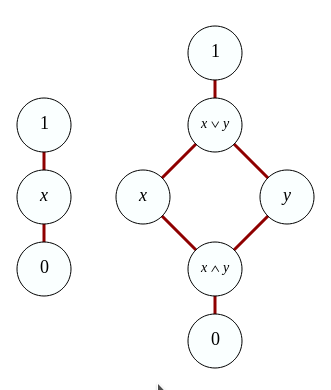
\includegraphics[width=0.7\textwidth,height=0.7\textheight,keepaspectratio=true]{figures/lattice.png}
\caption{An illustration of the free bounded distributive lattice over generating sets of dimension variables $I=\emptyset$,$I=\{x\}$, $I=\{x,y\}$ and $I=\{x,y,z\}$ by writing edges $a \rightarrow b$ if and only if $a \leq b$. A lattice is a partially ordered set in which all nonempty finite subsets have both a supremum and an infimum. Every free bounded lattice generated by a set $I$ gives rise to a De Morgan algebra $dM(I)$ by defining $\wedge$ as the infimum of the lattice and $\vee$ as the supremum of the lattice. Illustration taken from \cite{Eppstein2010}.}
\end{figure}

The involution of an element $x$ in a free De Morgan algebra is sometimes 
denoted by $1-x$ instead  of $\neg x$. Viewing a De Morgan algebra as a lattice with extra operations (see \Cref{lattice}), the involution can be seen as vertical mirroring within the lattice). When viewing the dimension variable $x$ as a line in a cube, the involution of $x$ represents the inverted line. 

\begin{definition}[Category of cubes]\label{cubcat}
  The category $\cube$ contains as objects the  finite subsets $I \subset 
\mathbb{A}$, called \keyword{dimension names}. Morphisms in this category are maps into De Morgan algebras: given two objects $I,J \in \cube$, $f 
\in \text{Hom}_{\cube}(J,I)$ if and only if $f: I \rightarrow dM(J)$ is a 
set map.
  \begin{itemize}
  \item  If $f \in \homo{\cube}{J}{I}, g \in \homo{\cube}{K}{J}$, 
the composition $g \circ f$, written as $fg$, is defined as the composition  
of set maps $\hat{g} \circ f$, where $\hat{g}$ is the extension of the set map $g$ to the free De 
Morgan algebra $dM(J)$.
    \item The identity map in this category is just the identity set map.
\end{itemize}
    \end{definition}

From now on, until the rest of this chapter, the symbol $\cube$ will be 
used to denote the category defined in \Cref{cubcat}. The category $\cube$ can be 
interpreted as an abstract higher-dimensional cube on which it is possible to 
apply operations described by a De Morgan algebra. As a base category it has 
much more objects and morphisms than the category that was used to construct 
directed and reflexive graphs, see \Cref{reflgraph}. As a consequence, types in 
a pre-sheaf model over this category will be more complicated than in 
\Cref{depgraphdiag}.

Now a few examples will be given of morphisms that are present in this category 
and will be used in the rest of the text.

\begin{example}
Let $I \subseteq J$. If $i \not \in I$ then the morphism $s_i : I \cup \{i\} 
\rightarrow I$ is defined as the set map associated to the inclusion $I \subset 
dM(I\cup \{i \})$.  Given $i \in I$ and $r \in dM(J)$, the morphism $(i/r): I 
\rightarrow dM(J) $ maps the dimension name $i$ on the element $r$ of the free 
De Morgan algebra $dM(J)$ and leaves other names untouched. These maps are also 
called \keyword{substitutions} although they are not exactly the same as 
context substitutions. 
\begin{itemize}
\item The \keyword{face maps} are compositions of substitutions $(i/b)$ where 
$b\in \left\{0,1\right\}$. These maps give the sub-faces or edges of a 
higher-dimensional cube.
\item The substitutions $(i / 1- i)$ can be interpreted as reflections along 
the $i$-axis or dimension of a cube. When intensional 
identity type will be modelled with higher-dimensional cubes, the terms will 
correspond with edges on a cube or paths and this substitution can be used to 
model the reverse path or equality.
\item The substitutions $(i / i \wedge j)$ extend a line parametrized by $i$ to 
a square depending on $j$ as well.
\end{itemize}

\end{example}

In pre-sheaf models of type theory, the contexts, types and terms of the type 
theory are modelled with pre-sheaves. In the cubical set model, the pre-sheaves 
are taken over $\cube$.

\begin{definition}\label{cubset}
A \keyword{cubical set} $\Gamma$ is a pre-sheaf $\Gamma \in \psh{\cube}$.
\end{definition}


In \Cref{cubset}, the contexts of the pre-sheaf model $\psh{\cube}$ are defined (see \Cref{premodel} for the definition of a pre-sheaf model). $\psh{\cube}$, which is actually a category with families, is denoted in this notation by only referring to the contexts. A pre-sheaf model that models a particular type theory should also have type and term functors (see \Cref{type_functor}) that model the right types, in this case $\psh{\cube}$ models the types of univalent type theory. These necessary types and functors of $\psh{\cube}$ will be described in the next sections. Because $\psh{\cube}$ models actually more than just univalent type theory, the type theory modelled is another type theory, called \keyword{cubical type theory}. This type theory forms an extension of cubical type theory and is defined in \Cref{ctt}.

First, some consequences of the choice of base category $\cube$ from \Cref{cubcat} in $\psh{\cube}$ will be studied. Given two finite sets of dimension variables $I,J \in \cube$ and a cubical set $\Gamma \in \psh{\cube}$,
there is an element $\rho \in \Gamma (I)$. Using the assumption that $\Gamma$ 
is a covariant functor, every substitution $f \in \homo{\cube}{I}{J}$ 
gives a set map $\Gamma (f) : \Gamma (I) \rightarrow \Gamma (J)$. 
The application of $\Gamma(f)$ to the object $u \in \Gamma (I)$ is written on 
the right and the context $\Gamma$ is implicit: $\rho f \in \Gamma(J)$. 

\begin{example}[Faces of cubes]\label{cubfaces}
If $I = \left\{x,y \right\}$, it is possible to interpret $u \in \Gamma(I)$ as 
a square with an edge $u(x/0)$ and corner $u(x/0)(y/0)$. In 
general, $u\in \Gamma (J)$ behaves like a $|J|$-dimensional cube and the face 
maps give faces of this cube.
\end{example}

Another example gives an interpretation to the unknowns of polynomial rings as faces of cubes:

\begin{example}[Polynomial rings]
Let $R$ be a commutative ring with a unit element. Define for $I$ a finite set 
of unknowns $\left\{x_1 , ..., x_n \right\}$, the set $R[I]$ of all polynomials 
in these unknowns. Then $R[-]$ can be considered as a functor and even a 
cubical set. For example, if $p(x,y,z) = 1 + x^2y +z \in R[x,y,z]$, it is 
possible to apply the face map $(y/0)$ to obtain $(1+x^2 y +z ) (y/0) = 1+z$.
\end{example}

\section{The face lattice}

The faces described in \cref{cubfaces} are put into a lattice structure to be able to use them in computations. Remember that a lattice is a partially ordered set in which all nonempty finite subsets have both a supremum and an infimum. 

\begin{definition}\label{facelattice}
The \keyword{face lattice} $\mathbb{F}$ is the distributive lattice generated 
by the face maps (which are the substitutions of the form $(i/b), i\in 
\mathbb{A}, b \in \left\{ 0,1 \right\}$). An element of the lattice $\varphi 
\in \mathbb{F}$ is called an \keyword{extent}. The top element in this lattice 
is denoted by $1_{\mathbb{F}}$ and the bottom element by $0_{\mathbb{F}}$ but 
the reference to $\mathbb{F}$ is often omitted in literature. The face lattice 
also satisfies $(i/0) \wedge (i/1) = 0_{\mathbb{F}}$ by definition. 
\end{definition}

The face lattice gives rise to a cubical set. For a $I\in 
\cube$, set $\mathbb{F}(I)$ to be the subset of extents in 
$\mathbb{F}$ that only contains dimension names $i \in I$. If $f \in 
\homo{\cube}{J}{I}, \mathbb{F}(I) \rightarrow \mathbb{F}(J): \varphi 
\mapsto f(\varphi)$ where $f$ just substitutes the symbols in $\varphi$ and 
applies the rewriting rules on \cite{Orton2019}, p. 39: given $r,s \in J$,

$$\begin{aligned}(r \vee s)/1 & \mapsto(r/1) \vee(s/1) \\(r \wedge s)/1 & \mapsto(r/1) \wedge(s/1) \\(1-r)/1 & \mapsto r/0 \end{aligned}$$
 
$$\begin{aligned}(r \vee s)/0 & \mapsto(r/0) \wedge(s/0) \\(r \wedge s)/0 & \mapsto (r/0) \vee(s/0) \\(1-r)/0 & \mapsto r/1 \end{aligned}$$

On the other hand, $\mathbb{F}$ can also be seen as a type in $\psh{\cube}$. 

Remember from \Cref{premodel} that in such a pre-sheaf model, contexts are 
pre-sheaves and types are pre-sheaves over a category of elements. The contexts 
in $\psh{\cube}$ are in \Cref{cubset} 
denoted by ``cubical sets".

The interpretation of the empty context $()$ in this pre-sheaf model is by 
\Cref{precon} a pre-sheaf denoted by $1$ that maps all objects in the base 
category $\cube$ to the same set containing one element, for example $\singleton$. 

To define $\mathbb{F}$ as a type in the empty context within the pre-sheaf 
model $\psh{\cube}$, it is necessary to describe how $\mathbb{F}$ acts on the category of 
elements. By definition of the category of elements (see \Cref{catel}), 
$$\int_{\cube} 1 = \left\{ (I, \rho ) \mid I \in \cube, \rho \in 1I 
\right\} \cong \left\{ (I, \star ) \mid I \in \cube \right\}  \cong 
\cube$$ where the last isomorphism is just a bijection that works by 
sending $(I, \star )$ to the set $\mathbb{F}(I)$.


\begin{definition}\label{interval}
The \keyword{interval object} $\mathbb{I}$ represents the unit interval. It is 
modelled as a context in $\psh{\cube}$. Such a model is a functor  
$\cube \rightarrow \set : I \mapsto dM(I)$.  $(i=0)$ acts as a term 
$\mathbb{I} \vdash (i = 0) : \mathbb{F}$ on elements $\rho \in dM (I)$. This 
map is defined as the map setting all the occurrences of $i$ in $\rho$ to $0$ 
and applying the rules of the distributive lattice.
\end{definition}

The interval object (or any other context) can also be seen as a type in the empty context $() \vdash \mathbb{I}$. In this interpretation it is a functor  $\int_{\cube} \Gamma \rightarrow 
\set : (I,\rho) \mapsto dM(I)$.



\section{Restricting contexts and types}

It would now be possible to describe how traditional types that are defined in 
(univalent type theory) can be interpreted in $\psh{\cube}$. 
However, the face and interval objects form a very important part of cubical 
type theory because of their interaction with other contexts. To understand 
this interaction, it is necessary how types interact with contexts in general.  

$\psh{\cube}$ also contains the context extensions from 
\Cref{preext}: if $\Gamma \vdash A$ is a type, then the context extension is 
defined by $$(\Gamma . A)(I) = \left\{ (\rho , u ) \mid \rho \in \Gamma (I), u 
\in A (I,\rho) \right\}.$$
Given $\Gamma \vdash A$ and an interpretation in $\psh{\cube}$, there is 
always a term $q$ in $$\mathbb{\Gamma}, A \vdash q : A.$$ This is used in 
$\psh{\cube}$ in combination with the interval object to parametrise 
terms and types by dimension variables. For example, if $\Gamma$ is any context, 
there is the type $\Gamma \vdash \mathbb{I}$ and an extension $\Gamma. 
\mathbb{I}$ but also a term $\Gamma. \mathbb{I} \vdash q : \mathbb{I}$.
r $(\Gamma, q : \mathbb{I})$ where $q$ is as before but depends on the context 
$\Gamma$ and type $\mathbb{I}$. In this situation and in literature $q$ is 
replaced by a letter $i,j,k$ and written in the context extension part. More 
precisely one writes $\Gamma, (i: \mathbb{I})$ instead of $\Gamma . 
\mathbb{I}$. If 

In $\psh{\cube}$, there is another way to form new 
contexts using extents. But to introduce this formally, it is necessary to 
pinpoint how extents are interpreted as terms.

\begin{definition}
In general, the type $\Gamma \vdash \mathbb{F}$ is defined in $\psh{\cube}$ by the contra-variant functor $$\mathbb{F} : \left\{ (I, \rho) \mid  I \in 
\cube,  \rho \in \Gamma (I) \right\} \rightarrow \set: (I, \rho) \mapsto 
\mathbb{F}(I)$$ where $\rho$ is just ignored. Terms $\Gamma \vdash \varphi : 
\mathbb{F}$ are defined by a dependent function $$\varphi : (I : \cube) 
\rightarrow (\rho : \Gamma (I)) \rightarrow  \mathbb{F}(I,\rho): I \mapsto \rho 
\mapsto \varphi \rho $$ where $I$ is implicit.

To calculate with $\varphi$, it is necessary to give a precise interpretation in 
$\psh{\cube}$. Define $ 0_{\mathbb{F}}, 
1_{\mathbb{F}} \in \mathbb{F}$ to be terms $0,1 : \mathbb{F}$ in $\psh{\cube}$ by 
setting \(0 \rho = 0, 1 \rho = 1\) for all $\rho \in \Gamma (I)$, $\Gamma \in 
\psh{\cube}$ and $I \in \cube$.  

For other extents, the definition or interpretation can depend on the context. 
When $\varphi$ is an extent containing only variables $i,j,k \in \mathbb{A}$, 
there is a term $(i: \mathbb{I}), (j: \mathbb{I}), (k: \mathbb{I}) \vdash 
\varphi : \mathbb{F}$ also denoted $(i,j,k: \mathbb{I}) \vdash \varphi : 
\mathbb{F}$. It's interpretation in $\psh{\cube}$ is as follows: take an $I \in \cube$ and  $\rho \in (i,j,k: \mathbb{I})$, then $\rho = 
((\rho_i, \rho_j), \rho_k)$, where $\rho_i \in dM(I)$, $\rho_j \in 
\mathbb{F}(I,\rho_i)$ which means that $\rho_j$ is an extent that only uses the 
variables in $I$. Further on, $\rho_k \in \mathbb{F}(I, (\rho_i, \rho_j))$. Now 
it is possible to define $\varphi(I,\rho)=\varphi(I,(\rho_i,\rho_j,\rho_k))$ as 
the extent where every variable $i$ occurring in $\varphi$ is replaced by the 
corresponding $\rho_i$ and apply the rules on \cite{Orton2019}, p. 39.
\end{definition}



\begin{definition}\label{contextrestriction}
Given a context $\Gamma \in \psh{\cube}$ and term $\Gamma \vdash \varphi : \mathbb{F}$, it is 
possible to define a new context $(\Gamma , \varphi)$, called the 
\keyword{context restriction by extent $\varphi$}. It is defined as  $$(\Gamma 
, \varphi)(I) = \left\{ \rho \in \Gamma (I) \mid \varphi \rho = 1_{\mathbb{F}} 
\in \mathbb{F}(I) \right \} .$$
\end{definition}
 
\begin{example}
Let $\Delta \equiv (\mathbb{I}, (i=0))$. Then 
$\Delta \cong ()$ as contexts.
\end{example} 

\begin{proof}
It remains to prove that there is a natural transformation between the 
two functors. First it has to be proven that for all $I \in \cube$, the 
sets $\Delta (I)$ and $()(I)=\{\star \}$ are isomorphic. In other words, it is 
necessary prove that the set $\Delta (I)$ exactly contains one element. But by 
definition of the interval object and the context restriction $\Delta (I) = 
\left\{  \rho \in dM(I) \mid (i=0) \rho = 1 \right\}$. But the only way that 
this could lead to $1$ is when $\rho = 1$. So $\Delta (I)$ contains one element: 
$\rho = i \vee 1$. It is still necessary to verify the commutativity properties 
of the natural transformation.
\end{proof}
 
 Similarly, it can be proven that the context $(i: \mathbb{I}, i=0, i=0)$ is 
isomorphic to the context $(i : \mathbb{I}, i = 0)$. 
 
There is an inclusion of the restricted context in the original context using a 
context morphism $\iota_{\varphi} : (\Gamma , \varphi ) \rightarrow \Gamma $. 
Intuitively, this restricted context can be used to define types and terms that 
are only defined the faces of the higher-dimensional cube $\Gamma$ specified by 
the extent $\varphi$.  

\begin{example}
A term $i : \mathbb{I}, j: \mathbb{I} \vdash a : A$ can be thought of as a 
square that is indexed by dimension variables $i$ and $j$. The top and left 
sides of the square are described by the lattice formula $\varphi = (i=0) \vee 
(j=1)$. So if the attention has to be restricted to these sides, it is possible 
to look at $a$ in the restriction of the original context: $i , j : \mathbb{I}, 
 \varphi \vdash a : A$. This is illustrated in \Cref{topleft}.
\end{example}

\begin{figure}
\centering
\includegraphics[width=0.8\textwidth]{figures/topleft}
\caption{An illustration of the context restriction by $\varphi = (i=0) \vee 
(j=1)$ coming from \cite{Orton2019}.\label{topleft}}
\end{figure}


The operation of extending (actually restricting) a context by an extent, can 
be viewed as a typing rule: 


\begin{prooftree}
\AxiomC{$\Gamma \vdash \varphi : \mathbb{F}$}
\UnaryInfC{$ \Gamma , \varphi \vdash $}
\end{prooftree}




\begin{definition}
Let $\Gamma \vdash A$ and $\Gamma \vdash \varphi : \mathbb{F}$.  A term $u$ is 
called a \keyword{partial element of extent $\varphi$}  if it is a term $( 
\Gamma, \varphi ) \vdash u : A{\iota}_{\varphi}$.
\end{definition}

There is also another definition of a partial element \cite{Orton2019}. This 
alternative definition let's the choice of $u$ depend on $\rho \in \Gamma (I)$. 

\begin{definition}
Let $\Gamma$ be context and $I \in \cube, i \not \in I, \rho \in \Gamma 
(I \cup \{i\}), \varphi \in \mathbb{F}(I)$. A partial element $u$ of $A(\rho)$ 
is a family $u_f \in A(\rho f)$ for every $f: J \rightarrow I \cup \{i\}$ such 
that $\mathbb{F}(s_i \circ f)(\varphi) = 1 _ {\mathbb{F}}$, with the property 
that for any $g:K \rightarrow J$,  $u_{f\circ g} = A(g)(u_f)$. Call 
$\varphi$ the \keyword{extent} of the partial element $u$.
\end{definition}


For each $\Gamma \vdash u : A$ and extent $\varphi$, there is partial element 
of extent $\varphi$, or term $(\Gamma, \varphi) \vdash u{\iota}_{\varphi} : 
A{\iota}_{\varphi}$. When a term $(\Gamma, \varphi) \vdash v : 
A{\iota}_{\varphi}$ is induced by a restriction by an extent $\varphi$, or in 
other words $v = u{\iota}_{\varphi}$, $v$ is called \keyword{extensible}. This 
can be intuitively seen as $v$ being extendible to $u$ by dropping the 
restriction by the extent $\varphi$. In type notation this relation between $u$ 
and $v$ is written as $\Gamma \vdash u : A [ \varphi \mapsto v ]$ expressing 
that $\varphi$ extends the term $v$ through $\varphi$. This can clarify the use 
of the word extent.

This specific notation for extents does not really state the presence of new 
types, contexts or terms in the model but can also be seen as a typing rule and 
written with natural deduction: 

\begin{prooftree}
\AxiomC{$\Gamma \vdash v : A$}
\AxiomC{$\Gamma , \varphi \vdash v = u : A$}

\BinaryInfC{$\Gamma \vdash u : A\ [ \varphi \mapsto v ] $}
\end{prooftree}

\begin{definition}[Generalized extent]\label{genextent}
A generalization of extents, in this text called \keyword{generalized extent}, is given in \cite{Huber2016}, p. 95 and can be summarized as follows:

\begin{prooftree}
\AxiomC{$\Gamma \vdash a : A$}
\AxiomC{$\Gamma, \varphi_i \vdash a = u_i : A, \quad i=1,...,k$}
\BinaryInfC{$\Gamma \vdash a : A\ [\varphi_1 \mapsto u_1 ,..., \varphi_k 
\mapsto u_k]$}
\end{prooftree}

\end{definition}

\begin{definition}[System introduction rule]
Assume that the following terms are given: 
\begin{itemize}
\item for each $1 \leq i \leq n$, there is a term  $\Gamma, \varphi_i \vdash 
t_i : A$ that is only defined on the extent $\varphi_i$, 
\item the extents cover the whole hypercube: $\Gamma \vdash \varphi_1 \vee ... 
\vee \varphi_n = 1_{\mathbb{F}} : \mathbb{F}$ 
\item the definitions are compatible $\Gamma, \varphi_i \vdash t_i = t_j : A, 
\forall 1\leq i,j\leq n$, 
\end{itemize}
Then there exists a term of type $A$, called a \keyword{system}, which  is denoted 
by $[\varphi_1 \  t_1, ..., \varphi_n \ t_n]: A$. This term also has to satisfy
\end{definition}

This term also has to satisfy the elimination rules mentioned in \cite{Huber2016}, figure 6.4.  A system allows to treat compatible terms, terms that agree at all points of the hypercube, as one term. The following lemma proves that compositions can be treated as generalized extents.



\begin{lemma}\label{extentrewrite}
Let $\Gamma \vdash \varphi : \mathbb{F}$ and $\Gamma \vdash A$. If $\varphi = 
\bigvee_i \varphi_i$ and $\Gamma \vdash \varphi_1 \vee ... \vee \varphi_n = 
1_{\mathbb{F}} : \mathbb{F}$, then the following types are logically equivalent: 
\begin{itemize}
\item $A\ [\varphi \mapsto [\varphi_1 \ t_1, ..., \varphi_n \ t_n]$
\item $A\ [\varphi_1 \mapsto t_1, ..., \varphi_n \mapsto t_n]$
\end{itemize}

\end{lemma}

It is believed but has not yet been completely verified that this follows from the definition of generalized extents and the elimination rule in \cite{Huber2016}, p. 95, figure 6.4 which states for any valid expression $J$: 
\begin{prooftree}
\AxiomC{$\Gamma, \varphi_i \vdash J, 1 \leq i \leq n $}
\AxiomC{$\Gamma \vdash \varphi_1 \vee ... \vee \varphi_n = 1_{\mathbb{F}} : 
\mathbb{F}$}
\BinaryInfC{$\Gamma \vdash J$}
\end{prooftree}


\begin{example}
The notation $[(i = 0) \vee (i=1) \mapsto [(i=0) \ u, (i=1)\  v]$ can 
be replaced by $[i=0 \mapsto u, i=1 \mapsto v]$. This is done very often in 
\cite{Huber2016} and implementations \cite{Moertberg2018}.
\end{example}


\section{Adding operations}\label{extraops}

The category theoretical interpretations of other 
terms and types in $\psh{\cube}$ will not be studied yet. In $\psh{\cube}$, types have an intuitive description as cylinders. When $\Gamma \vdash A$ is a type in $\psh{\cube}$, it is described by a functor from the category of elements 
$$\text{Ty}:\int_{\cube} \Gamma \rightarrow \set.$$ This is noted as $A(\rho) \in \set$ for some $|I|$-dimensional hypercube $\rho 
\in \Gamma (I)$. At the same time the substitutions that apply to objects in $\cube$ and substitute dimension variables can 
be lifted by \text{Ty} to the level of types. 

\begin{example}
Let $\Gamma  \in \psh{\cube}$ and a type $\Gamma \vdash A$. If $I=\{x\}$ is one dimensional and $\rho \in \Gamma(I)$, substitutions $(x/r)$ that 
map the dimension variable $x$ on $0$ or $1$ can be visualized as mapping $\rho$ on the endpoints of an edge. The lift $A(\rho)$ is mapped by $(x/r)$ on the faces of the 
cylinder similarly to the action of the morphisms $f$ and $g$ in \Cref{depgraphdiag}. Another way to interpret the type $A$ is using \Cref{typelemma} by viewing the type $A$ as a new context $\Delta$.  This is visualized in \Cref{hubtypes}. 
\end{example}

\begin{figure}\label{hubtypes}
 \centering
 \includegraphics[width=0.5\textwidth]{figures/typecylinder}
 \caption{Picture taken from \cite{Huber2016def}.}
\end{figure}

The interesting properties of univalent type theory and the 
consequences of the univalence axiom all follow from the intensional identity 
type and its typing rules. The intensional identity type of univalent type 
theory can be modelled in $\psh{\cube}$ but it is special in the following 
sense. Given a type $A$ and terms $a,b,c:A$, the interpretation of the 
intensional identity type $a =_A b$ and $b=_A c$  in cubical sets is only 
transitive if $A$ satisfies a \keyword{Kan extension property} (see 
\Cref{fig:Kan}). This property of types $A$ tells how the terms of $A$ can be 
extended from a restricted context cube to a full cube. It is made precise with 
a composition and filling operation on the types and terms in $\psh{\cube}$.

% a c
% b c cube
\begin{figure}
\begin{centering}
\includegraphics[width=0.3\textwidth]{figures/Daniel_Kan.jpg}
\par\end{centering}
\caption{\label{fig:Kan}Daniel Kan (1927-2013) was a Dutch category and homotopy theorist. He defined his Kan extension property  in the context of algebraic 
topology for cubical sets, see his book \cite{Kan1955} saying how boxes can be 
filled. Although \cite{Coquand2019} mentions a predecessor to this property in 
\cite{Eilenberg1939}. This Kan extension property later involved into different 
flavours such as a version for simplicial sets stating that every ``horn'' can 
be filled and the composition operation, see \Cref{compdef}. Picture taken in his home in 
Massachusetts by \cite{Kan2005}.}
\end{figure}

Adding \keyword{operations} to $\psh{\cube}$ is done by adding axioms stating 
the existence of certain structures, sets, functors or elements, satisfying 
properties that are related to the properties of the type system that is 
modelled. Operations will be denoted with another font type. To arrive at a 
complete model of univalent type theory, including the univalence axiom, also a 
glue operation has to be added to $\psh{\cube}$ (see \Cref{glueOp}). 

\subsection{The composition operation}

The most important operation in $\psh{\cube}$ is the composition operation 
\cite{Orton2019}. The semantics of the composition operation are as follows:

\begin{definition}\label{compdef}
Let $\Gamma \in \psh{\cube}$ be a context. A \keyword{composition structure} for $\Gamma \vdash A$ is an operation, 
$\op{comp}$, that depends on the following elements:

\begin{itemize}
\item $I \in \cube, i \not \in I, \rho \in \Gamma(I \cup \{i\}), \varphi 
\in \mathbb{F}(I)$, where $\rho$ can be seen as an ($I$+1)-dimensional 
hypercube.
\item $u$ a partial element of $A(\rho)$ of extent $\varphi$ and $a_0 \in 
A(\rho (i/0))$ such that for all $f:J\rightarrow I$, $A(f)(a_0) = u _{(i/0) 
\circ f}$ and $\mathbb{F}(f)(\varphi) = 1_{\mathbb{F}}$. Here $u$ can be viewed 
as a set of values for $A$ on sides $\varphi$ of $\rho$ that takes values $a_0$ 
on the bottom of $\rho$ described by $i=0$. The value $a_0$ has to agree with 
the values $u$ on other sides.
\end{itemize}

Then there is a set element $\op{comp}(I,i,\rho,\varphi, u,a_0)\in 
A(\rho(i/1))$. This element is uniform in the sense that for any $f:J 
\rightarrow I$ and $j \not \in J$: 

\begin{itemize}
\item $\op{comp} \left(I,i,\rho,\varphi, u , a_0 \right) f = 
\op{comp}(J,j,\rho(f \cup (i/j)), \varphi f, u(f \cup (i/j)), a_0 f)$  where $f 
\cup (i/j): J \cup \{j\} \rightarrow I \cup \{i\}$ is just the extension of $f$ 
with the substitution $(i/j)$ and $u(f \cup (i/j))$ is the partial element 
defined for $g: K \rightarrow J$ as $u_{(f \circ g \cup (i/j))}$.

\item $\op{comp}(I,i,\rho, 1_{\mathbb{F}}, u, a_0) = u_{(i/1)}$. In other 
words, the values of $A$ on top of the hypercube $\rho$ can be extended to to 
values on top of the faces of the hypercube $\rho$ for which $i=1$. In other 
words, it is possible to close the ``lid'' of the box $\rho$ along the side 
$i=1$.

\end{itemize}



\end{definition}



Again, it is possible to write this operation with natural deduction as a introduction rule telling the 
existence of the category theoretical interpretation in $\psh{\cube}$ of a specific 
term with a specific type. 

\begin{definition}[Composition introduction rule]
The notation $\op{comp}(I,i,\rho, \varphi, u, a_0)$ 
is written with a shorter syntax and with application to $\rho$ implicit as 
$\compt{i}{A}{\varphi}{u}{a_0}$.

\begin{prooftree}
\AxiomC{$\Gamma \vdash \varphi : \mathbb{F}$}
\AxiomC{$\Gamma , i : \mathbb{I} \vdash A$}
\AxiomC{$\Gamma, \varphi, i : \mathbb{I} \vdash u : A$}
\AxiomC{$\Gamma \vdash a_0 : A(i/0)[\varphi \mapsto u(i/0)]$}

\QuaternaryInfC{$\Gamma \vdash \op{comp}^i A [ \varphi \mapsto u ] a_0 : A(i/1) 
[\varphi \mapsto u(i/1)] $}
\end{prooftree}

If $\sigma : \Delta \rightarrow \Gamma$ is a context substitution, then this 
morphism acts on terms as follows:

\begin{prooftree}
\AxiomC{$\left( \op{comp}^i A [ \varphi \mapsto u ] a_0 \right)\sigma$}
\UnaryInfC{$\op{comp}^j A(\sigma,i/j) [\varphi \sigma \mapsto u(\sigma, i/j)] 
a_0 \sigma$}
\end{prooftree}

where $j$ does not appear as a dimension variable in a syntactical 
representation of $\Delta$ yet. For types the morphism acts analogously. 
\end{definition}


The existence of a composition structure for all types in $\psh{\cube}$ cannot be taken for granted. Its 
existence depends on the choice of context and type.

\begin{definition}
A \keyword{Kan type} or \keyword{fibrant type} $A$ is a type for which there 
exists a composition structure $\op{comp}_A$.
\end{definition} 


\subsection{The path type}\label{pathtypes}

The use of the identity type in cubical type theory is replaced by the use of a path type. There is also a naming problem because cubical type theory is modelled by $\psh{\cube}$ which is a pre-sheaf models and the standard 
pre-sheaf model of the identity type is defined as a functor $\op{Id}$: if $\Gamma \vdash A$, $\Gamma \vdash a : A$ and $\Gamma \vdash b : A$, then 
$$\left(\texttt{Id}_A(a,b) \right)\rho = \left\{ \star \mid a\rho = b\rho \right\}$$

However, the type modelled by the functor $\op{Id}$ does not satisfy the 
properties of the intensional identity type in univalent type theory. It does 
for example only admit at most one term and satisfies the uniqueness of 
identity proofs principle (and also \Cref{axiomk}). This means it is 
incompatible with the univalence axiom and insufficient to model univalent type 
theory. 

To solve these problems in $\psh{\cube}$ and other pre-sheaf models, 
another interpretation is given to the identity type. This interpretation is 
done with a functor that models the intensional identity type between terms 
$a,b:A$ correctly (up to the computation rule \Cref{pathindprop}) is called 
$\pa{A}{a}{b}$. 

\begin{definition}\label{pathdef}
Given terms $\Gamma \vdash a,b : A$, the \keyword{path type} $\op{Path}_A(a,b)$ 
is defined as follows:
\begin{itemize}
\item Given $\rho \in \Gamma (I), \op{Path}_A(a,b)(\rho)$ is the set of 
equivalence classes generated by pairs $(i, w)$ with $i\not \in I$ and $w \in 
A(\rho s_i)$ such that $w(i/0) = a(\rho)$ and $w(i/1)=b(\rho)$, where 
$(i,w)$ is identified with $(i',w')$ if and only if $w'=w(i/j)$. 

\item The action of $\op{Path}_A(a,b)$ on a morphism $f:(J,\rho,f) \rightarrow 
(I,\rho)$ is given by $(i,w)f \equiv (j, w(f \cap (i/j))$ for $j \not \in J$.
\end{itemize}
The equivalence class of $(i, w)$ is also denoted by $\left< i \right> w$ where 
$w$ implicitly depends on a choice of $\rho$. Formally, using typing rules and 
natural deduction: 

\begin{prooftree}
\AxiomC{$\Gamma \vdash A$}
\AxiomC{$\Gamma, i : \mathbb{I} \vdash t : A$}
\AxiomC{$\Gamma, i : \mathbb{I} \vdash t(i/0) = a : A$}
\AxiomC{$\Gamma, i : \mathbb{I} \vdash t(i/1) = b : A$}
\QuaternaryInfC{$\Gamma \vdash \left< i \right> t : \pa{A}{a}{b}$}

\end{prooftree}

\begin{prooftree}
\AxiomC{$\Gamma \vdash t : \pa{A}{u_0}{u_1}$}
\UnaryInfC{$\Gamma \vdash t 0 = u_0 : A$}
\end{prooftree}

\begin{prooftree}
\AxiomC{$\Gamma \vdash t : \pa{A}{u_0}{u_1}$}
\UnaryInfC{$\Gamma \vdash t 1 = u_1 : A$}
\end{prooftree}


\end{definition}


To obtain a model for intensional identity type that also satisfies the 
computation rule of the intensional identity type (see \Cref{pathindprop}), the 
identity type of Swan \cite{Swan2014} has to be used instead of the path type 
in \Cref{pathdef}. The identity type of Swan does exactly have the elimination 
rule of \Cref{pathindprop}. However, the difference between the path type in 
\Cref{pathdef} and the identity type of Swan is only minor (up to paths) and 
will not be covered thoroughly in this text. Both Swan's identity type and the 
path identity type in \Cref{pathdef} are logically equivalent, meaning that 
they can be substituted by each other. See  \cite{Huber2016}, p. 114 for a 
comparison of both types and the more advanced text \cite{Swa18} about a 
general framework for choosing identity types. In this text, the notation $a 
=_A b$ or simply $a = b$ will be used for both Swan's identity type 
(constructed by Swan) and the path identity type between terms $a, b: A$ defined 
in this section. 

The standard term of the path type $\op{Path}_A(a,a)$ between a term $a : A$ 
and itself  is the reflexive term $\op{refl}_A(a)(I,\rho) \equiv (i, a(\rho 
s_i))$ for some $i \not \in I$. It is in \cite{Huber2016}, p. 90 also denoted 
by $1_a$.

This definition applies to any type, but to have that the path type is Kan type 
and satisfies all the properties of the intensional identity type in univalent 
type theory, it is necessary that the original type to which the path type is 
applied has a composition structure or is Kan. If the original type was not 
Kan, the path type would for example not necessarily be transitive. It is proven in \Cref{pathtransitivity} that it is enough to make the path type transitive.


\begin{example}\label{pathtransitivity}

The \keyword{transitivity} property of equality, in this case the transitivity of the path type, 
states that if $\Gamma \in \psh{\cube}$, $\Gamma \vdash a,b,c : A$, $p: \op{Path}_A(a,b)$ and $q: 
\op{Path}_A(b,c)$, there is a term $r : \op{Path}_A(a,c)$. If $A$ is Kan, then 
$\op{Path}_A$ is transitive.	

\begin{proof}
The proof is illustrated in \Cref{transdiag}.

\begin{figure}\label{transdiag}
\[ \begin{tikzcd}
a \arrow[r, dashrightarrow] 
& c  \\
a 	\arrow[u, "refl"]	
	\arrow[r, "p \  i"]
& b  \arrow[u, "q \ j"] 
\end{tikzcd}
\] 

\caption{Transitivity can be modelled in $\psh{\cube}$ by a  composition 
of paths along the edges of a square. Assume that $i$ is the horizontal axis and   $j$ the vertical axis, then the composition operation $\texttt{comp}$ gives the closing lid: $p \cdot q$, proving transitivity. Diagram inspired by \cite{Cohen2016}, 
section 4.3.}
\end{figure}

If $A$ is a Kan type, by definition, it has a composition operation. The 
syntactical object $u = [i=0 \mapsto a, i=1 \mapsto q j]$ can be viewed as a 
term that is only defined on three sides:

\begin{itemize}
\item The extent $\varphi = (i=0) \vee (i=1)$ defines two sides of the 
hypercube. On these sides the values of $u$ vary along a second dimension $j$. 
This is written as $\Gamma, (i=0)\vee (i=1), j : \mathbb{I} \vdash u$.
\item On the side $j=0$ the values of $u$ coincide with the values of the path 
$p$. This means that for fixed $i$, in type notation $\Gamma \vdash (p \  i) : 
A(j/0)[\varphi \mapsto u(j/0)]$

\end{itemize}

For fixed $i$, take $a_0 = p \  i$. The composition operation now gives a 
term that extends $u$ along the remaining side $j=1$: $$\op{comp}^j\ A\ [(i/0 
\mapsto a, (i/1) \mapsto q\ j] (p\ i)$$ which can be rewritten using  
\Cref{extentrewrite} as $$\op{comp}^j A [(i/0) \mapsto a, (i/1) \mapsto q \ j] 
(p \  i) \equiv z.$$ The term $z$ is of type $A(j/1)[i=0 \mapsto a, i=1 \mapsto 
c]$.

If this term depends on $i$, the introduction rule of a 
path can be applied to return a term denoted by $\left< i \right> z$ that has 
type $\pa{A}{a}{c}$. To verify this it is necessary to check that the endpoints 
of this path $\left< i \right> z$ are indeed $a$ and $c$.

The endpoints are obtained by applying the context morphisms $$(i/0),(i/1): 
(\Gamma . ( j : \mathbb{I})) \rightarrow (\Gamma. ( j : \mathbb{I}) . ( i :  
\mathbb{I}))$$ to the generalized extent judgement $$(\Gamma. ( j : \mathbb{I}) 
. ( i :  \mathbb{I})) \vdash z : A(j/1) [i =0 \mapsto a, i=1 \mapsto c].$$ The 
application of a context morphism $\sigma$  is just the application of $\sigma$ 
to each judgement contained in the generalized extent, which are by \Cref{genextent}
(omitting $(\Gamma. ( j : \mathbb{I}) . ( i :  \mathbb{I}))$):

\begin{itemize}
\item $ () \vdash z: A(j/1)$
\item $ (i = 0) \vdash z = a : A(j/1)$
\item $ (i = 1) \vdash z = c : A(j/1)$
\end{itemize}

These judgements and the introduction rule of the path type in \Cref{pathdef} prove that $z$ is the right path, making the transitivity 
property hold for $\op{Path}$. 

\end{proof} 

\end{example}

If $A$ is Kan, it can be proven that the path type $\op{Path}_A(a,b)$ not only  
satisfies transitivity but also all the typing rules of  the intensional 
identity type (as mentioned in \Cref{equalitytype} or
\cite{Orton2019}, p. 35) except the computation rule. However, it is not known if the Kan property and the composition structure are necessary for this property of the identity type to hold in $\psh{\cube}$, and 
whether the composition operation can be weakened. 

In \cite{Cavallo2019}, the composition operation of $\psh{\cube}$ is weakened to a \keyword{weak composition operation}. This allows to develop a type theory 
in which the mathematical properties of the different cubical type theories can 
be studied simultaneously, see for example the alternative theory described in 
\Cref{comptt}.


\subsection{The filling operation}\label{filling}

The composition operation of a Kan type extends the definition of a partial 
term from one that defined only on one  endpoint  of a dimensional variable to 
one that is also defined on the other endpoint of the dimension variable. It 
however only gives the lid of the box as described in 
\Cref{pathtransitivity} which is actually the example  on \cite{Coquand2018}, 
page 10. 

Complementary to the composition operation, there is a filling operation in $\psh{\cube}$ that 
not only ``fills'' the endpoints but also covers the interior of partial terms 
that are defined on hypercubes by introducing a new variable dependency in the 
context. This operation is used in \cite{Coquand2018} for the definition of 
higher inductive types. The filling operation makes use of the lattice 
structure that is defined in \Cref{lattice}. 

% See \Cref{zeroPath} of an example of how the $\wedge $ and $\neg$ operation 
% can be used.

% \begin{figure}\label{zeroPath}
%  \centering
% \begin{tikzpicture} [decoration={markings,mark=at position 0.5 with {\arrow{>}}},
   witharrow/.style={postaction={decorate}},
   dot/.style={draw,fill,circle,inner sep=1.5pt,minimum width=0pt}
  ]
		\begin{pgfonlayer}{nodelayer}
		\node [style=none] (0) at (0, -0) {};
		\node [style=none] (1) at (3, -0) {};
		\node [style=none] (2) at (0, 3) {};
		\node [style=none] (3) at (3, 3) {};
		\node [style=none] (4) at (1, 2) {};
		\node [style=none] (5) at (2, 1) {};
		\node [style=none] (6) at (2, 0) {};
		\node [style=none] (7) at (0, 2) {};
		\node [style=none] (8) at (0, 3) {};
		\node [style=none] (9) at (1, 3) {};
		\node [style=none] (10) at (1, 3) {};
		\node [style=none] (11) at (2, 3) {};
		\node [style=none] (12) at (2, 3) {};
		\node [style=none] (13) at (-2, -1) {};
		\node [style=none] (14) at (1, -1) {};
		\node [style=none] (15) at (-4, -0) {};
		\node [style=none] (16) at (-1, -0) {};
		\node [style=none] (17) at (-4, 3) {};
		\node [style=none] (18) at (0.75, -0) {};
		\node [style=none] (19) at (3, 2) {};
		\node [style=none] (20) at (3, 0.75) {};
		\node [style=none] (21) at (0, 1) {};
	\end{pgfonlayer}
	\begin{pgfonlayer}{edgelayer}
		\draw [style=simple] (0.center) to node[left]{$\texttt{P\ 0\ j}$} (2.center);
		\draw [style=arrow] (0.center) to node[above]{$\texttt{P\ i\ 0}$} (1.center);
		\draw [style=simple] (2.center) to node[above]{$\texttt{P\ i\ 1}$} (3.center);
		\draw [style=arrow] (3.center) to node[right]{$\texttt{P\ 1\ j}$} (1.center);
		\draw [style=arrow] (2.center) to node[below]{$\texttt{P}$} (1.center);
		\draw [style=arrow] (13.center) to node[below]{$\texttt{A\ i}$} (14.center);
		\draw [style=arrow] (15.center) to node[left]{\texttt{j}} (17.center);
		\draw [style=arrow] (15.center) to node[below]{\texttt{i}} (16.center);
		\draw [style=arrow] (7.center) to (4.center);
		\draw [style=arrow] (9.center) to (4.center);
		\draw [style=arrow] (11.center) to (5.center);
		\draw [style=arrow] (21.center) to (5.center);
	\end{pgfonlayer}
\end{tikzpicture} 

% 
%  
%  0 ---- 0 ---- 0	
% |      |      |
% |      |      |
% 0 --- 1/2 -- 1/2    
% |      |      |
% |      |      |
% 0 --- 1/2 --- 1
% 
%  
%  
%  \caption{If $A$ depends on $i \in dM(\{i,j\})$ (see \Cref{freedm}), it is 
% possible to ``square'' $A$ in Agda-Cubical syntax \cite{Moertberg2018} with 
% lattice operations $\wedge$ and $\neg$ to a square $P$. At each vertical 
% line in % this ``square", there is line going from $A(i)$ to $A(0)$ defined by 
% $\texttt{P % i}$ and in the direction of the arrows. It is important to keep in 
% mind that % this square is only a geometrical realization of a discrete concept. 
% In reality % there are only $0$ and $1$'s. }
% \end{figure}

% Let's say that $f : \mathbb{I} \rightarrow \mathbb{I}$ is a classical unary 
% function, a function taking one argument. It is possible to turn $f$ in to a 
% binary function, taking two arguments, by setting $\hat{f} : \mathbb{I} 
%\times % \mathbb{I} \rightarrow \mathbb{I}: (i,j) \mapsto f(\text{min}(i,j))$. 
%Visually % speaking, assuming that $\mathbb{I}=[0,1]$, there is a diagram of the 
%values of % $\hat{f}$.
% 
% \unsure{Didn't I do this before}
% 
% \[ \begin{tikzcd}
% (0,1) \arrow[r, "f(i)" ] 
% & (1,1)  \\
% (0,0) 	\arrow[u, "f(0)"]	
% 	\arrow[r, "f(0)"]
% & (1,0)  \arrow[u, "f(j)"] 
% \end{tikzcd}
% \]
% 
% 
% In practice, in cubical type theory $f$ will be a path

For \Cref{filldef}, the lattice structure defined in \Cref{lattice} has to be 
used. The use of the $\wedge$ lattice combinator is illustrated in 
\Cref{twopath}.

\begin{figure}\label{twopath}
\centering
\[ \begin{tikzcd}
p (0) \arrow[r, "p" ] 
& p(1)  \\
p(0) 	\arrow[u, "p(0)"]	
	\arrow[r, "p(0)"]
& p(0)  \arrow[u, "p"] 
\end{tikzcd}
\]
\caption{Take two terms $a,b:A$ and a path $p : \pa{A}{a}{b}$, then the term 
$p(i/i\wedge j)$ is a two-dimensional path that takes two arguments $i$, $j$ 
and returns values based on the interpretation of $i \wedge j$ as 
$\text{min}(i,j)$. The two-dimensional path $p(i/i\wedge j)$ can be 
illustrated as a square taking $i$ as a horizontal axis and $j$ as a vertical axis.}
\end{figure}


\begin{definition}\label{filldef}
Let $A$ be a Kan type. The Kan \keyword{filling} operation on $A$ is an 
operation that returns a term. More specifically, set 
$\fillt{i}{A}{\varphi}{u}{a_0}$ to be the term $$\op{comp}^j \ A(i/i \wedge j) 
\ \left[\varphi \mapsto u(i/i \wedge j), (i=0) \mapsto a_0 \right] \ a_0 : A $$ 
in context $\Gamma . (i, j: \mathbb{I})$.
\end{definition}

Using the definition of extents, it is possible to decompose the filling term 
$v$ into judgements (omitting $\Gamma, i,j : \mathbb{I}$):

\begin{itemize}

\item The judgements $()\vdash v : A(i/i \wedge j)$ and $\varphi \vdash v = 
u(i/i \wedge j) : A(i/i \wedge j)$. 
This means that the term $v$ is defined on the interior $A(i/i \wedge j)$. 
Applying the substitution $(j/i)$ gives the usual composition term.

\item There is a judgement $(i = 0) \vdash v = a_0 : A(i/i \wedge j)$ that is 
equivalent with $$() \vdash v(i/0) = a_0 : A(i/0).$$
Now $a_0\rho$ is on the left side of the hypercube $\rho \in \Gamma \left( 
\left\{i,j\right\} \right)$.

\end{itemize}

The filling is the composition plus something else, also called the interior. 
But the interior in this context is not the interior in a topological sense 
because there is no concept of continuity or topology present in $\psh{\cube}$. In $\psh{\cube}$ it is only 
possible to compute with a finite amount of (subsets of) corners of 
standardized hypercubes.

The existence of Kan types, types with a composition operation is not so 
straightforward. For each type that is used in a type system and has a valid 
interpretation in $\psh{\cube}$, the composition operation 
has to be defined. Examples of such composition structures for natural numbers 
and path types can be found in \cite{Huber2016}, Sec. 6.4.5, p. 97-98. Once 
these composition structures are given for all basic types in intensional type 
theory, including paths, the category with families model is strong enough to 
model univalent type theory. However, the univalence axiom is an axiom about 
universes of intensional type theory and universes are also types. So it is 
necessary to define a composition structure for universes in $\psh{\cube}$. This composition structure is 
defined in \cite{Huber2016} with the help of a \texttt{Glue} type which will be 
introduced in \Cref{glueOp}. 



\subsection{The $\op{Glue}$ type}\label{glueOp}



Now that the path type of intensional type theory has been modelled in $\psh{\cube}$ (omitting the definitions of dependent product and sum types that are given for general pre-sheaf models in \cite{Huber2016}, Sec. 1.2), the concepts from \Cref{contractible} can be translated to their analogue in $\psh{\cube}$. This will be done by treating $\psh{\cube}$ as a type theory (cubical type theory) with the help of typing rules (syntax). The 
definition of a term of contractibility in intensional type theory is 
$$\op{isContr} \ A = (x:A) \times \left( (y:A) \rightarrow \pa{A}{x}{y} 
\right)$$ and is a valid expression in cubical type theory because sum types 
and path types have a valid interpretation in cubical sets.

Similarly, a function $f:T \rightarrow A$ is an \keyword{equivalence} if and 
only if the following type is inhabited $$\isequiv{T}{A}{f} = (y: A) 
\rightarrow \op{isContr} ((x:T) \times \pa{A}{y}{f \ x}$$  and an equivalence 
in general is a term of the type $$\op{Equiv} \ T \ A = (f:T\rightarrow A) 
\times \isequiv{T}{A}{f}.$$ 
 

There is a semantic interpretation of the $\op{Glue}$ type given in \cite{Huber2016} but this will be skipped because it is quite 
complicated and does not add much intuition for the value of this type in the 
context of the proof of univalence. The text \cite{Orton2019}, Ch. 5-6, 
tries to simplify the semantics of the $\op{Glue}$ type using topoi. The 
introduction of the $\op{Glue}$ type is given in \cite{Orton2019}, p. 30.

\begin{definition}[\texttt{Glue} introduction rule]
Assume that a (total, not 
necessarily partial) type $\Gamma \vdash B$ is given together with another type that is partial 
$\Gamma, \varphi \vdash A$ for some extent $\varphi$. If the partial type is 
equivalent to the total type $\Gamma, \varphi \vdash f : \op{Equiv} \ A \ B $ 
as far as it is defined, there is a type $\Gamma \vdash \op{Glue} \ \left[ 
\varphi \mapsto \left( A, f \right) \right] \ B$ that satisfies certain 
elimination rules. 

This can also be expressed with natural deduction as:

\begin{prooftree}
\AxiomC{$\Gamma \vdash \varphi : \mathbb{F}$}
\AxiomC{$\Gamma \vdash B$}
\AxiomC{$\Gamma, \varphi \vdash A$}
\AxiomC{$\Gamma, \varphi \vdash f : \op{Equiv} \ A \ B $}
\QuaternaryInfC{$\Gamma \vdash \op{Glue} \ \left[ \varphi \mapsto \left( A, f 
\right) \right] \ B$}
\end{prooftree}

\end{definition}


 


Another way to phrase this is as follows: the introduction rule of the $\op{Glue}$ type tells that given an element of 
the face lattice $\mathbb{F}$ expressing the sides of a square on which $f$ is 
defined as an equivalence $A\rightarrow B$, there is a bigger type that ``glues 
the sides together''. It is a bigger type because by one of the eliminating typing rules as mentioned on \cite{Huber2016}, figure 6.5, the 
$\op{Glue}$ type extends the partial type $A$. More precisely, it says that for 
$\varphi = 1_{\mathbb{F}}$, there is $\Gamma \vdash \left[ 1_{\mathbb{F}} 
\mapsto (T,f) \right] \ B = A$. Terms of the $\op{Glue}$ type come into two 
forms:

\begin{itemize}
\item If it is known whether $B$ has a particular partial type, there is a typing 
rule giving a $\op{glue}$ term. More precisely, if $t$ is a term of $A$, $f$ 
is the equivalence and $\Gamma \vdash b : B \  \left[ \varphi \mapsto f \ a 
\right]$, then there is a term denoted by $\op{glue} \ [\varphi \mapsto a ] \ 
b$ of the glue type. 
\item The $\op{unglue}$ term functions as an inverse of this term, a computation typing rule. For example, given a $\op{Glue}$ term $c : \op{Glue} \ 
[\varphi \mapsto (A,f)] \ B$, the term $\op{unglue} \ c$ is of type $B \ 
[\varphi \mapsto f\ c]$.
\end{itemize}

\begin{example}

Take $\varphi = (i=0) \vee (i=1)$. Then the type $A$ is only defined for $i = 
0$ or $i =1$, so there are two sides of the hypercube on top of which the type $A$  and the partial equivalence $f$ are
defined. The values of $A$ on top of these sides are called $A_0$ and $A_1$. The 
values of $B$ are computed with substitutions. The partial equivalence $f$ also has 
values $f_0$ and $f_1$. Let $\op{G} = \op{Glue} \  [i = 0 \mapsto 
(B(i/0),f_0), i=1 \mapsto (B(i/1), f_1)]$, then this can be illustrated:

\[ \begin{tikzcd}
A_0 \arrow[r, dashed, "\op{G}" ] \arrow[d, "f_0"]	
& A_1  \arrow[d, "f_1"]  \\
B(i/0) 	
	\arrow[r, ""]
& B(i/1)  
\end{tikzcd}
\]

%\unsure{I don't get example on Huber2016, p. 101}

\end{example}

As it goes for all the types that are introduced in cubical type theory, it is 
also necessary to introduce a composition operation for the $\op{Glue}$ type. 
This is done on \cite{Huber2016}, Sec. 6.6.2 and makes the $\op{Glue}$ type 
into a Kan type.

The only remaining step to do is to prove that the universe type of $\psh{\cube}$ is also Kan, 
which is done in \cite{Huber2016}, Sec. 6.7.2. Once the composition and 
glueing operations are defined for the universe types, they are defined for all 
types. As explained in \Cref{pathtransitivity}, this implies that the path type 
over universes also satisfies transitivity. This means the model described in 
this section supports all types from intensional type theory, the 
\texttt{Glue}-type and a composition structure:

\begin{definition}[\cite{Huber2016}]\label{ctt}
A \keyword{cubical type theory} is an 
extension of intensional type theory (see \Cref{typetheory}) with the following 
properties:
\begin{itemize}
 \item All types from intensional type theory, including natural numbers, 
dependent sum and product types, are modelled in $\psh{\cube}$ (see \Cref{cubcat}) by defining them as functors (see also \cite{Huber2016}, 
p. 28-30).
 
 \item The intensional identity type is modelled by modifying the path type of 
which the semantics and typing rules are given in \Cref{pathtypes}.
 
 \item There are the following additional objects that are not present in intensional 
type theory or homotopy type theory:
 
 \begin{itemize}
 \item The objects $\mathbb{F}$ and $\mathbb{I}$ introduced in 
\Cref{facelattice,interval} and the context restriction 
\Cref{contextrestriction}.
  \item The \texttt{Glue} type from \Cref{glueOp} allows the construction of a 
proof of univalence, see \Cref{univalenceproof}.
 
 \end{itemize}
 \item Every type (excluding \(\mathbb{F}, \mathbb{I}\) has a composition operation (is a Kan type), 
satisfying the typing rules (and semantics) in \Cref{compdef}, allowing the path identity type (and the intensional identity type constructed from the path identity type) to be transitive which makes cubical type theory a proper 
extension of intensional type theory.
\end{itemize} 
\end{definition}

The theory in \Cref{ctt} (in which the univalence axiom is provable) 
satisfies \keyword{canonicity of numerals} (see \Cref{canonicity}). 


The proof of univalence described in \Cref{univalenceproof} was not established in one paper but it took a while until the right syntax and semantics was found to be able to speak of cubical type theory as in $\Cref{ctt}$.

\subsection{Historical development of cubical set models}\label{nominalmod}

The first time dimension variables or cubes were used in type theory was in \cite{bernardy2012computational}. The theory of \keyword{nominal sets} which is introduced in \cite{Pitts:2013:NSN:2512979} introduced a way of working with dimension variables as objects in a category. In \cite{Bezem2014}, this idea was extended to a categorical model of type theory in cubical sets together with Kan extension properties. The way nominal sets were used in \cite{Bezem2014} was discussed in \cite{Pit14}. Cubical sets were however already discussed in \cite{GraMau03}. The model was extended in \cite{huber2015model} to include more detailed proofs and semantics of the universe. In \cite{Coq13} it was suggested how this model could be allow a proof of the univalence axiom. By that time there was already an implementation of \cite{huber2015model} available in \cite{Huber2014} and later \cite{Moertberg2015}. A formal written proof of univalence with this model was given in \cite{Bezem2018} but slightly more complicated than in later models and higher inductive types could not yet be modelled. 

This earlier model was however valuable because it proved the consistency of cubical type theory relative to the framework of category theory in cubical sets. It also did not use choice principles which made it the first constructive model of the univalence axiom and univalent type theory. Models of type theory in type theory that do not use any extra structure on the base category are called \keyword{monoidal} or sub-structural because they can be represented using only products of an interval object.


 
%The talk \cite{altenkirch2014syntax} investigated how the typing rules of a cubical type theory should look like with applications in parametricity. The paper \cite{Licata2015} applied a version of cubical type theory for synthetic homotopy theory. 

The \keyword{lattice structure} in  \Cref{lattice} was the first step in allowing higher inductive types and simplifying operations. It was  was historically 
later introduced by \cite{Cohen2016} and slightly corrected in \cite{Huber2016} for simplifying composition and using 
higher inductive types. There is still research going on on whether the lattice structure is necessary in the base category and other models such as \cite{Altenkirch2015} do not make used of it.
There is an unpublished comparative study in \cite{Awodey2016June} on choices of base categories that are related to the base categories used in \cite{Bezem2014} and \cite{Huber2016}. Each choice of a variation of the base category can lead to more desirable properties of the type theory being modelled but no better alternative has been found yet (a choice that results in a more efficient cubical type theory). For example, \cite{Gun2019} uses twisted cubes to model directed (cubical) type theory.

The latest version of cubical type theory that is implemented in proof assistants has slightly different operation than described in \cite{Huber2016}. To allow working with higher inductive types, \cite{Huber17note} suggested to decompose the composition operation in a homogeneous composition and a generalized transport. This idea was worked out in \cite{Coquand2018}. Since then, no big changes were made to the semantics but there is still research on models that can unify the semantics of cubical type theory and variations such as two-level (cubical) type theory in \cite{Uem19} and \cite{Cavallo2019}. %There  is also a successor to the presheaf model developped in \cite{awodey_2018}, called a \keyword{natural model}. This model could simplify the semantics of thec urrent cubical set model. 


\chapter{Proof of univalence}\label{univalenceproof}

Cubical type theory was invented to give a ``computational interpretation of 
the univalence axiom'' which would allow to compute with expressions in 
univalent type theory. In this section, an overview will be given of 
historical attempts to this proof and one of the most recent versions of the 
proof.


\section{The univalence theorem}

Remember from \Cref{uniaxiom} that the \keyword{univalence} theorem in cubical 
type theory (which is an axiom in univalent type theory) states:

\begin{theorem}
 Given two types $A, B : \mathcal{U}$ of the same universe, there is an 
equivalence between the types $A = B$ and $A \simeq B$.
 \end{theorem}

Because it can be proven in certain models such as \cite{Kapulkin2012} and 
cubical type theory as in \Cref{ctt}, the axiom can also be called a theorem 
within a particular model. In this section, the proof of the theorem in 
\cite{Moertberg2018} will be discussed.

\subsection{History of the proof}

In this section, the development of the most recent revision of the proof in  \cite{Moertberg2018}, \texttt{Cubical.Foundations.Univalence} as of writing this 
text will be discussed. For a history of the development of the semantics, see \Cref{nominalmod}.

The first model in which this theorem became provable was simplicial sets 
\cite{Kapulkin2012}. The proof in simplicial sets used the ideas such as the 
\text{Glue} type that were reintroduced in later proofs in cubical sets, see 
\cite{Huber2016}, p. 103-104 and p. 122-123 or \cite{Bezem2018} for an approach 
without lattice structure (mentioned in \Cref{nominalmod}). 

The proof in \cite{Huber2016} was the first one that was formally verified in a 
type theory, more specifically cubical type theory. The first part of this proof has since been rewritten 
in \cite{Weinberger2016}. The formalization has been continuously worked on 
since \cite{Moertberg2015} and \cite{Cohen2016} in \cite{Moertberg2018}. Recently, this library code was surveyed in \cite{Moertberg2018a} but later revisions of the files in this library can have made this explanation less up-to-date. In the following sections the different parts of the implementation the proof will be discussed.

\section{Proof of the univalence theorem}

\subsection{Contractibility of equivalence singletons}

\begin{theorem}[\texttt{unglueIsEquiv}]
Let $\Gamma, \varphi \vdash f : T \rightarrow A$ be a partial equivalence with 
extent $\varphi$. The function $$ \op{unglue} : \op{Glue} \ \left[\varphi 
\mapsto (T,f) \right] \ A \rightarrow A$$ is an equivalence. 
\end{theorem}

Another proof is \cite{Huber2016}, p. 103, Thm 6.7.2 and uses two extra 
lemmas to construct to proof the equivalence.

\begin{proof}
As mentioned in \Cref{contractible,uniaxiom}, an equivalence is a function with contractible  fibres (pre-images). So, to prove that 
\texttt{unglue} is an equivalence amounts to proving that for any $b$ in the 
co-domain $A$, the fibre $\op{fiber}\ \op{unglue} \ b$ is contractible. In 
other words, the following proofs have to be given:
\begin{itemize}
\item A point  $x : \op{fiber}\ \op{unglue} \ b$. 
\item A proof that given $y : \op{fiber}\ \op{unglue} \ b$, $x = y$. 
\end{itemize}
The point $x$ is constructed by constructing the \texttt{glue} term on top of 
$\texttt{hcomp} \ u \ b : A$ where $\op{u}$ is a partial term. It has to be 
proven that this term is indeed in the fibre. For the second part, an arbitrary 
element of the fibre $y$ is taken. Now a path is constructed that is point-wise 
defined with a partial term \texttt{u'} and $\op{glue}$ terms. The end points 
of this path are indeed $x$ and $y$ because $\op{u'}$ extends $\op{u}$. There 
also have to be proofs that the terms on the path are in the fibre (or 
pre-image of $b$). These proofs are built with an application of $\op{hfill}$, 
a formalization of the filling operation described in \Cref{filling}.
\end{proof}

Now $\op{unglueEquiv}$  expresses that any partial family of equivalences can 
be extended to a total one.

The following theorem is an intermediate statement of the univalence axiom that 
is more directly provable than the traditional statement. It will function as a 
lemma for proving the more traditional version of the univalence axiom.

\begin{theorem}[\texttt{EquivContr}]\label{contrSingl}
 $$\forall A : \type_l, \op{isContr} \ \left( \sum \ (T : \type_l) \  \left( T 
\simeq A \right) \right).$$ 
\end{theorem}


The proof in \cite{Huber2016}, p. 104, Cor. 6.7.3 uses an extra lemma.

\begin{proof}
It is necessary to give a term $x : \sum \ T : \type \  \left( T \simeq 
A \right)$ and a proof that there is an equality between $x$ and any other term 
$y$ of the same type. Take the trivial equivalence  $(A, \op{idEquiv})$ for 
$x$. It remains to prove that every other term is equal to this one. So take 
another term $$\op{y : Σ\ (Set\ l)\ (λ T → T ≃ A))}$$ then it can be shown with 
$\op{unglueIsEquiv}$ that there is a path $(A , \texttt{idEquiv}\ A) \equiv y$.
\end{proof}


According to \cite{Huber2016}, \cite{Voevodsky2013}, Thm. 5.8.4, it should 
follow that the equivalence type forms an identity system. The statement of the 
univalence theorem is however not immediate.

The path type in cubical type theory can be slightly modified (see 
\Cref{pathtypes}) such that it satisfies the J-eliminator, see 
\Cref{pathindprop}. Equivalences also satisfy an eliminator, called 
\keyword{equivalence induction}. 

\begin{theorem}[\texttt{EquivJ}]
Given a property $P: (A \ B : \mathcal{U}) \rightarrow (e : B \simeq A) 
\rightarrow \mathcal{U}$, a proof of the base step $r : (A : \mathcal{U}) 
\rightarrow P \ A\ A \ (\texttt{idEquiv} \ A)$, then it is possible to produce 
a proof of the property for any $A \ B: \mathcal{U}$: $$ P\  A \ B\ e.$$
\end{theorem}

\begin{proof}

For the proof, some lemmas are needed: 
\begin{itemize}

\item The lemma $\op{idIsEquiv}: \forall A \in \type , \op{isEquiv} \  
(\lambda \ x \mapsto x)$ proves that the identity map is is an equivalence. This also an immediate proof of the reflexivity of equivalences which is formalized in  $\op{idEquiv}: \forall A : \type, A 
\simeq A$.

\item Applying \Cref{contrSingl} to some type $B$ gives a proof of 
contractibility of a sum type depending on $B$. More precisely, there is a $(C, 
C \simeq B)$ with $C:\mathcal{U}$ such that every other $C'$ gives an equality 
$(C,C \simeq B) = (C',C'\simeq)$. Contractibility is very similar to being an 
h-prop. The theorem $\op{isContr} \rightarrow \op{isProp}$ which is stated in 
\texttt{Cubical.Foundations.HLevels} converts proofs of contractibility into 
proofs of being an h-prop using the composition operation. It shows that any 
terms of this particular sum type over $B$ are connected by a path or equality.


\item   Assuming $e : A \simeq B$, the above theorem is applied to connect the 
tuples $(B, \op{idEquiv} \ B)$ and $(A, e)$ by an equality in the proof of 
theorem $\op{contrSinglEquiv}$.

\item Transport is used in the form of $$\op{subst} : \left(B : A \rightarrow \type 
\right) (p : x = y) \rightarrow B \ x \rightarrow B \ y.$$ This theorem is part 
of a few theorems that are all formalizations of univalent type theoretical 
transport in defined with the composition operation in 
\texttt{Cubical.Core.Prelude}.

\end{itemize}

Eventually the J-combinator for equivalences is defined by transporting the 
base case $r$ over the equality returned by $\texttt{contrSingleEquiv e)}$.

\end{proof}

This construction of the map $\op{ua}$ is based on the one defined in 
\cite{Huber2016}, Ex. 6.6.2, p. 101.

\begin{definition}
$\op{ua} : \forall \ A\ B:\type, A \simeq B \rightarrow A = B$ is defined with 
the $\op{Glue}$ type. The definition can be illustrated with a diagram:



\[ \begin{tikzcd}
A \arrow[r, dashed, "\op{ua}" ] \arrow[d, "e"]	
& B  \arrow[d, "\op{idEquiv} \ B"]  \\
B	
	\arrow[r, ""]
& B  
\end{tikzcd}
\]

The implementation of the definition takes a partial equivalence $e$ and type 
$A$, a dimension variable or parameter $i$ and maps it on a term $\texttt{ua e}$ of type $\op{Glue} \ [(i = 0) 
\mapsto (A,e), (i=1) \mapsto (B, \op{idEquiv} \ B)] \ B$.  By the elimination rules of the \texttt{Glue} type given on \cite{Huber2016}, Fig. 6.5, $\texttt{ua e}$ is a path with 
endpoints $A$ and $B$. 
\end{definition}


$\op{uaIdEquiv} : \forall A, \op{ua}\ (\op{idEquiv}\ A) = \op{refl}$, where 
$\op{refl}$ is the reflexive path or equality. It tells that the reflexive 
equivalence is mapped onto the reflexive identity by $\op{ua}$.

\begin{definition}
An \keyword{isomorphism}  (or \keyword{homotopy equivalence}, 
\keyword{quasi-inverse} \cite{Voevodsky2013})  is defined in 
\texttt{Cubical.Foundations.Isomorphism} as a function $f : B \rightarrow A$ 
with a pseudo-inverse $g : B \rightarrow A$ such that $f\circ g$ and $g \circ 
f$ are both homotopic to the identity map. 
\end{definition}

The theorem $\op{isoToIsEquiv}$ is a proof that any isomorphism $f: A 
\rightarrow B$ is an equivalence.



\begin{example}
Let $A = \op{Bool}$ and $B = \op{Fin}\ 2$. It is possible to prove that $A = 
B$. This is done using any bijection between $A$ and $B$ which is also an 
isomorphism. Such an isomorphism is also an equivalence and applying the map $\op{ua}$ returns path of type $A = B$.
\end{example}

\subsection{Conclusion of the proof}

Using the previous lemmas and results, the statement and proof of the 
univalence theorem is now much easier.

\begin{theorem}[\texttt{Univalence.thm}]
Given a function  $$\op{au} : A = B \rightarrow A \simeq B$$ and a proof that 
$\op{au}$ maps the $\op{refl} : A = A$ identity type constructor onto the 
constant equivalence $A \rightarrow A$, the theorem $\op{Univalence.thm}$ 
states that $\op{au}$ is an equivalence.
\end{theorem}

\begin{proof}
First it is shown that the given map $\op{au}$ has to be an isomorphism with as 
inverse the previously constructed map $\op{ua}$. An isomorphism is the 
homotopy type theoretic variant of a homotopy equivalence or more precisely, a 
bi-invertible map as in chapter 4 of \cite{Voevodsky2013}. To prove that 
\texttt{au} is a isomorphism, it is necessary to prove the left-inverse and 
right-inverse properties (up to a path). Both proofs use that $\op{compPath}$ 
is just the transitivity property of ``$=$" and congruence. 
\begin{itemize}
\item The left-inverse is proven with equivalence induction \texttt{EquivJ} on 
the property that \texttt{au} is a left-inverse for equivalences \texttt{e}: 
\texttt{au (ua e) ≡ e)}. 
\item The right-inverse is proven with equality induction \texttt{J} on the 
property that \texttt{ua} is a right-inverse for paths \texttt{p}: \texttt{ua 
(au p) ≡ p}. 
\end{itemize}
Although an isomorphism is not well-behaved (it is for example not a 
proposition), it contains more information than equivalence and from an 
isomorphism, an equivalences can be extracted. Applying $\op{isoToIsEquiv}$ 
gives that $\op{ua} : A = B \rightarrow A \simeq B$ is an equivalence or 
$\op{isEquiv}\ \op{ua}$. 
\end{proof}

The theorem of univalence is then a simple consequence of an application of 
\texttt{Univalence.thm}

\begin{theorem}[\texttt{univalence}]
Given any $A,B : \mathcal{U}$, there is an equivalence $\left( A \equiv B 
\right) \simeq \left( A \simeq B \right).$
\end{theorem}


\begin{proof}
The function $\op{lineToEquiv} : A = B \rightarrow A \equiv B$ that maps paths 
directly on an equivalence serves as a candidate for the inverse \texttt{au} in 
\texttt{Univalence.thm}. The necessary condition that is still needed to apply 
\texttt{Univalence.thm} is the fact that \texttt{lineToEquiv} maps the 
reflexive equality onto the trivial equivalence. This follows by proving that 
the underlying maps of the image under \texttt{lineToEquiv}, 
\texttt{pathToEquiv refl} and \texttt{idEquiv A} are equal with transport and 
using the fact that the property of being an equivalence is a proposition, 
which means there can only be one such proof, such that the the equivalences 
also have to be equal and \texttt{pathToEquiv refl ≡ idEquiv A}. The proof is 
formalized in \texttt{pathToEquivRefl}. Applying \texttt{Univalence.thm} to the 
map and this fact, gives a proof that \texttt{pathToEquiv} is an equivalence. 
Assembling this into an equivalence gives a term of the equivalence type 
\texttt{(A ≡ B) ≃ (A ≃ B)}, which is a proof of univalence.
\end{proof}

\subsection{Univalence with topoi}

The \keyword{language of topoi} can be used to discover more fundamental 
models of cubical type theory and univalence \cite{Orton2019}. A topos is a 
category that behaves like the category of sets. Examples of topoi are the 
category of sets and pre-sheaves. 

First, the cubical type theory as presented in \cite{Huber2016} and this text 
is translated in the  language of topoi \cite{Orton2019}, Sec. 5.3. Some 
definitions become much simpler such as the De Morgan algebra used for the base 
category and the face lattice that were presented in \Cref{facelattice} become 
\cite{Orton2019}, figure 5.4. This results in an alternative proof of 
univalence that can be more insightful \cite{Orton2019}, Sec. 5.5. An 
overview of related foundational work can be found in \cite{Pitts2018} and 
\cite{Licata2018}.


\section{Applications of the proof of univalence} \label{applications}

In \Cref{univalenceproof}, it was shown that the univalence axiom holds in 
cubical type theory. The theorem of univalence allows to use all the 
concepts from univalent type theory, also called homotopy type theory, in 
cubical type theory. Cubical type theory was implemented in 
\texttt{Cubical.Core.HoTT-UF} of \cite{Moertberg2018}.

In combination with the standard library of Agda \cite{Danielsson2019}, it is 
possible to produce concrete examples in univalent type theory of reasoning 
with univalence.

\subsection{Isomorphism invariant algebra}\label{magmas}

In the theories of groups and other algebraic structures, proofs are preferably 
done for only one structure in an isomorphism class. The proofs for other 
structures in the same class are not considered valuable because they do not 
add information. With the univalence axiom, it is possible to treat 
different proofs for properties of isomorphic structures as equal. In \cite{Danielsson2012} this was proven already but not yet for a constructive interpretation of the univalence axiom.

\begin{definition}
A \keyword{monoid} $A$ is a set $A$ with an associative binary operation $+_A$ and neutral element $0_A$. A monoid without neutral element is called a \keyword{semigroup} and a semigroup that is not necessarily associative is a \keyword{magma}. Given two monoids $A$ and $B$, an isomorphism $f : A \rightarrow B$ is:
\begin{itemize}
 \item a bijective set map $A \rightarrow B$.
 \item structure-preserving, $f(x +_A y) = f(x) +_B f(y)$ and $f(0_A) = 0_B$
\end{itemize}
\end{definition}
 
 
 
\begin{example}
The following two objects are monoids:
\begin{itemize}
 \item The usual natural numbers: $s_1  \equiv (\mathbb{N}, (m,n)\mapsto m+n, 0)$.
 \item The natural numbers without zero: $s_2 \equiv (\mathbb{N}_0, 
(m,n)\mapsto m+n -1, 1)$.
\end{itemize}
 Between these two monoids there is an isomorphism $f : s_1 \rightarrow s\_2 : n \mapsto n +1$. 
\end{example}


This example is mentioned in the introduction of \cite{Coquand2013} but it is not verified if it really works for their specific encoding of isomorphisms.


The goal of this section is to prove \Cref{magmatransp} in cubical type theory based on the progress of \cite{Danielsson2012}. There encoding in the standard library (file \texttt{Algebra.Structures} of \cite{Danielsson2019}) contains definitions for monoids and other algebraic 
structures as record types but uses an equivalence relation, also called \keyword{setoid encoding}. Because of the number of  laws that need to be 
supplied to define a monoid, the example was reduced to a custom definition of 
magmas. In the case of magmas, the setoid encoding is overcomplicated, so a simple custom definition of magmas was used instead, see \Cref{m2def}. 

\begin{figure}\label{m2def}
\begin{center}
\begin{BVerbatim}
op₂ : Op₂ ℕ₀
op₂ (suc x , _) (suc y , _) = ((suc (x + y))  , true)

s₂ : myMagma _ lzero
s₂ = record {
  Carrier = ℕ₀ ;
  _✧_ = op₂
  }
\end{BVerbatim}
\end{center}

 \caption{A magma $s_2$ in Agda is a term of the record type \texttt{myMagma}. This record contains the carrier set, the operator and groups them into one object.}
\end{figure}

\begin{theorem}\label{magmatransp}
Let $M$ be the type of magmas. Given two magmas $s_1$, $s_2$ and an isomorphism $f : s_1 \rightarrow s_2$, there is a term of the path type $s_1 =_M s_2$ (from \Cref{pathindprop}) and proof of properties $M \rightarrow \mathcal{U}$ can be transported along this path. 
\end{theorem}

More specifically, if there is a proof of the fact that $s_1$ is commutative, there is also a proof of the fact that $s_2$ is commutative. 




\subsubsection{Defining a path between structures}

In this section, \Cref{magmatransp} will be proven. More precisely, it will be explained how a term \texttt{algPath} of the type \texttt{s₁ ≡ s₂} can be defined in Agda. Such a term is path with endpoints $s_1$ and $s_2$ that coincides at time $i$ with a ``point-wise 
defined'' algebraic structure, a magma. So defining such path is equivalent 
with defining a magma at every time $i$ that coincides with the given $s_1$ and 
$s_2$ on its endpoints. To understand how this works, look at the definition of 
magmas as record types. Record types are nested dependent sums and a path 
between two terms of a dependent sum is composed of paths between the 
components of the dependent sum. So for each component of the record type there 
should be path, including the carrier sets and operators on both structures. 

It can be proven using the map $f: n \mapsto n + 1$ that there is an 
equivalence between $\mathbb{N}$ and $\mathbb{N}_0$ which gives by the 
univalence axiom (proven to hold in \Cref{ctt} by \Cref{univalenceproof}) a 
path $\texttt{ℕ ≡ ℕ₀}$. This gives a path between one component in the term of 
the record types of magmas. 

\begin{figure}\label{transpop}
\centering
\incfig{transport_arguments}
\caption{A visualization of the transports that are implemented in \Cref{zeroPathLift}.}
\end{figure}

Another component is the operator. In this case, the operator is actually a 
path between the two given operators \texttt{op₁} and \texttt{op₂}. This means that a point-wise defined 
operator has to be defined such that coincides with the respective operators on its endpoints. The construction of such an operator \texttt{opᵢ'} at time \texttt{i} is illustrated in \Cref{transpop} and implemented in \Cref{zeroPathLift} by:

\begin{enumerate}
\item Transport the arguments of the operator \texttt{opᵢ' i} over \texttt{zeroPath i} from the intermediate carrier set \texttt{fEq i} to the carrier set \texttt{fEq i0} which is just $\mathbb{N}$. 
\item Apply the usual summation of $\mathbb{N}$ defined by \texttt{op₁}.
\item Transport the result of the computation back to \texttt{fEq i}.
\end{enumerate}


\begin{figure}\label{zeroPathLift}
\centering 
\begin{BVerbatim}
zeroPath : (i : I) → (fEq i) ≡ ℕ
zeroPath i = λ j → fEq (i ∧ (~ j))
...
opᵢ' : PathP (λ i → Op₂ (fEq i))  op₁'  op₂'
opᵢ' i x y = transport (sym (zeroPath i))
    (op₁ (transport (zeroPath i) x) (transport (zeroPath i) y))
\end{BVerbatim}
\caption{This definition of an intermediate operator.}

\end{figure}

However, the operator \texttt{opᵢ'} from \Cref{zeroPathLift} does not have the operator \texttt{op₂} at its ending point. It is necessary to proof
that  \texttt{opᵢ' i1 ≡ op₂' ≡ op₂}. The proof of \texttt{op₂' ≡ op₂} is given in \Cref{adaptedOp}.

\begin{figure}\label{adaptedOp}
 \centering
\begin{BVerbatim}
endLemma : op₂' ≡ op₂
endLemma i x y =
  (op₂' x y
       ≡⟨  refl  ⟩
   transport fEq (op₁ (transport (sym fEq) x) (transport (sym fEq) y))
       ≡⟨ transpR (op₁  (transport (sym fEq) x) (transport (sym fEq) y)) ⟩
   f (op₁  (transport (sym fEq) x) (transport (sym fEq) y))
       ≡⟨ cong₂ (λ x y → f (op₁ x y)) (transpL x) (transpL y) ⟩
   f (op₁  (g x) (g  y))
       ≡⟨ gIsMorphism x y ⟩
   op₂ x y ∎) i

pathLemma : (PathP (λ i → Op₂ (fEq i)) op₁' op₂') 
    ≡  PathP ((λ i → Op₂ (fEq i))) op₁ op₂
pathLemma = 
    cong₂ (PathP (λ i → Op₂ (fEq i))) startLemma endLemma

opᵢ : PathP (λ i → Op₂ (fEq i)) op₁ op₂
opᵢ = transport pathLemma opᵢ'
\end{BVerbatim}

\caption{This lemma proves that the endpoint of the original 
intermediate operator \texttt{opᵢ'} is (path) equal to
\texttt{op₂}. This is used to define a new intermediate operator 
\texttt{opᵢ} for which \texttt{opᵢ i1 ≡ op₂}.}   
\end{figure}

The rest of the definition of the intermediate point-wise defined algebraic 
structure \texttt{algPath} of type \texttt{s₁ ≡ s₂} is straightforward and can be seen in \Cref{algpath}. 

\begin{figure}\label{algpath}
\centering
 \begin{BVerbatim}

algPath : s₁ ≡ s₂
algPath = λ i → record {
   Carrier = (fEq i) ;
   _✧_ = opᵢ i
   }
 \end{BVerbatim}

 \caption{A term of the intensional identity type between the two algebraic 
structures is a structure depending on a parameter \texttt{i} that has 
components depending on the parameter \texttt{i}. Each component was point-wise 
defined before and can be assembled into a point-wise structure.}
\end{figure}

\subsubsection{Transporting proofs}


An application of the path \texttt{s₁ ≡ s₂} between the two magmas, is that the 
proof of commutativity of the first magma \texttt{s₁} can be transported to a 
proof of the commutativity of the second magma \texttt{s₂}, defined as 
$$\texttt{com₂ = transport (λ i → isCommutative (algPath i)) com₁}.$$ See \Cref{comtrans} for the full code fragment. Although the 
property of being commutative is very simple, it can be generalized to more 
complicated properties and algebraic structures. The 
complete code of this implementation can be found on \cite{Van19} and verified 
with the installation instructions.

\begin{figure}\label{comtrans}
\begin{center}
\begin{BVerbatim}
isCommutative : ∀  {a l} → (myMagma a l) → Set a
isCommutative m = 
    (x y : (myMagma.Carrier m)) → 
    ((myMagma._✧_  m) x y) ≡ ((myMagma._✧_  m) y x)

com₁ : isCommutative s₁
com₁ = +-comm

com₂ : isCommutative s₂
com₂ = transport (λ i → isCommutative (algPath i)) com₁
\end{BVerbatim}
\end{center}
\caption{A magma is defined to be commutative if its operation is 
commutative on the carrier type. Commutativity for natural numbers has already 
been proven in the standard library. This proof can be transported along the 
term of equality \texttt{s₁ ≡ s₂} to give a proof of commutativity of 
\texttt{s₂}. Unfortunately, normalizing \texttt{com₂} results in a memory leak that may be caused by the implementation of cubical type theory in the underlying library \cite{Moertberg2018}. This also fails for concrete small values for \texttt{com₁}, for example \texttt{com₁ 4 6} but is currently being resolved.} 
\end{figure}

\subsubsection{Conclusion}

This example shows that it is possible to do a version of the ``isomorphism-invariant'' mathematics as claimed in \cite{Voevodsky2013} in practice with magmas using a constructive interpretation of the univalence axiom. 

The core requirements to be able to implement this example were
\begin{itemize}
 \item The construction of a homotopy type equivalence \texttt{f} between the carrier types. This is roughly a bijection for discrete set-like types or h-sets as defined in \Cref{hset}.
 \item A proof that the inverse to \texttt{g} is a morphism
 \item The proof of univalence and more specifically the \texttt{ua} map constructed with the \texttt{Glue} type. 
\end{itemize}

The construction in this example works by constructing a path of magmas. The paths between the components of the magmas are:
\begin{itemize}
\item a path between the carrier types constructed using \texttt{ua}.
\item an operator that starts and ends at the operators of the given algebraic structures defined using characterizations of left and right transport (see \Cref{leftrighttransp}).
\end{itemize}

This means that this implementation of two specific magmas could be likely generalized to general magmas, monoids and isomorphisms between these structures. For this, intermediate proofs for properties such as associativity and the neutral element  could be defined  with the lemmas of \Cref{leftrighttransp} and a similar proof as in \Cref{adaptedOp}. However, due to a lack of time this has not been tried explicitly yet.


\begin{figure}\label{leftrighttransp}
 \begin{center}
  \begin{BVerbatim}
transpR : (z : ℕ) → transport fEq z ≡ f z
transpR z = Univalence.uaβ fEquiv z

baseIndLemma : (A : Type _) → 
    (λ i → ua (idEquiv A) (~ i)) ≡ ua (invEquiv (idEquiv A))
baseIndLemma A = 
  sym ( ua (idEquiv A) ) ≡⟨ uaIdEquiv ⟩
  sym refl ≡⟨ refl ⟩
  refl ≡⟨ sym uaIdEquiv ⟩
  ua (idEquiv A) ≡⟨ cong ua (equivEq (idEquiv A) (invEquiv (idEquiv A)) refl) ⟩
  ua (invEquiv (idEquiv A)) ∎

transpLLemma₁ : sym (ua fEquiv) ≡ (ua (invEquiv fEquiv))
transpLLemma₁ = EquivJ
  (λ _ _ e → sym (ua e) ≡ ua (invEquiv e)) (λ A → baseIndLemma A) _ _ fEquiv 

transpL : (z : ℕ₀) → transport (sym fEq) z ≡ g z
transpL z =
  transport (sym fEq) z ≡⟨ (cong (λ p → transport p z) transpLLemma₁) ⟩
  transport (ua (invEquiv fEquiv)) z ≡⟨ refl ⟩
  transport (ua gEquiv) z ≡⟨ (Univalence.uaβ gEquiv z) ⟩
  g z ∎
  \end{BVerbatim}

 \end{center}
\caption{These lemmas proof that the transport used in \Cref{adaptedOp} are just applications of the given maps that are morphisms. To prove this lemmas it was necessary to use equivalence induction which is defined using a form of equivalence (based on a hint in \cite{Vez19} and meanwhile implemented in \cite{Moertberg2018})}
\end{figure}


Applying a (weak form of) the structure invariance principle in cubical type theory is not the easiest approach for proving algebraic properties up to isomorphism. However, not all structures in mathematics are as well-known as natural numbers and the structural and overly 
rigorous approach that such type theories require can be more beneficial in a 
general setting, see also the discussion in \Cref{futapp}.  At least in this case of simple traditional algebra, it seems 
easier to use specialized software such as \cite{TheGAPGroup2018} to carry out 
algebraic computations and proofs. There are other examples of property transports such as the implementation of a transport of properties between unary and binary encodings of natural numbers in the file \texttt{Data/BinNat/BinNat.agda} in \cite{Moertberg2018}.


\subsection{Generic datatypes}

Apart from mathematical applications, there are also more practical 
applications. Datatypes in mainstream programming languages such as Java can be 
parametrized by parameters. For example, a list can be parametrized by the type 
of it's contents. The resulting datatype is then called generic, the approach 
is called \keyword{generic programming}. There might be multiple ways of 
implementing a datatype and several implementations might be equivalent. This 
is were the univalence axiom comes into play. 

Assume two date representations are given: ``(month, day)" and ``(day, 
month)". These representations are equivalent by the swapping map. Univalence 
gives a path between the equivalent representations. Assume databases are 
generically defined for a certain date representation. For example, the type of 
databases is defined as $\op{List} \ (\mathbb{N} \times \op{String} \times (X 
\times \mathbb{N}))$ where $X = \mathbb{N} \times \mathbb{N}$ is any type of 
date representation. The goal is to prove that the databases given in table 
\ref{databases} are equal.

\begin{table}[]
\centering
\begin{tabular}{lllll}
\hline
\textbf{N.} & \textbf{Name} & \textbf{Day} & \textbf{Month} & \textbf{Year} \\ 
\hline
4           & John          & 30           & 5              & 1956          \\
%8           & Hugo          & 29           & 12             & 1978          \\
...  		& ...			& ...			& ...			& ...			\\
%15          & James         & 1            & 7              & 1978          \\
%23          & Jack          & 3            & 12             & 1969          \\
42          & Sun           & 20           & 3              & 1980          \\ 
\hline

\hline \\
\hline
\textbf{N.} & \textbf{Name} & \textbf{Month} & \textbf{Day} & \textbf{Year} \\ 
\hline
4           & John          & 5              & 30           & 1956          \\
%8           & Hugo          & 12             & 29           & 1978          \\
...  		& ...			& ...			& ...			& ...			\\
%15          & James         & 7              & 1            & 1978          \\
%23          & Jack          & 12             & 3            & 1969          \\
42          & Sun           & 3              & 20           & 1980          \\ 
\hline
\end{tabular}
\caption{The European and American databases on \cite{Licata2013}, p. 47. 
\label{databases}}

\end{table}


The path between representations is lifted to a path on the level of the type 
of databases. The lifted path becomes a path between two different databases 
using two different but equivalent representations. Because paths behave like 
equality, the two databases are equal. The example has been implemented in the 
file \texttt{Cubical.Experiments.Generic} of \cite{Moertberg2018}.

This simple example shows that the implementation of univalence in cubical type 
theory allows a programmer to treat generic datatypes as the same datatype up 
to equivalence of the parameter type.

\subsection{Formalizing algebraic topology}

\subsubsection{Higher inductive types}\label{hit}

Higher inductive types are a concept coming from \cite{Voevodsky2013}. A 
\keyword{higher inductive type} is a type that has formation and construction 
rules  as other types but these rules are accompanied by additional typing 
rules stating how to produce terms of the path types between its terms. In 
other words, the type is generated by constructors and equalities. Higher 
inductive types are useful in synthetic homotopy type theory.

The first attempts at using higher inductive types in the cubical pre-sheaf 
model date from \cite{Licata2015}, \cite{Huber2016} and \cite{Cohen2016} but it 
was only until recently that the semantics were worked out in \cite 
{Lumsdaine2017} and  \cite{Coquand2018}.



\begin{example}
The \keyword{circle} $S^1$ as a topological object is defined as line of which 
the endpoints are identified. In the language of higher inductive types this 
becomes two constructors: $\op{base} : S^1,  \op{loop} : \op{base} = \op{base}$.
\end{example}

\begin{example}
The \keyword{torus} is defined similarly but now there is an extra loop which is 
introduced with an extra constructor. In addition, both loops intersect, 
meaning that doing one loop is topologically equivalent to taking the other 
loop. This is written as a path that starts and ends at the second loop: 
$\op{square} : \op{PathP} \ (\lambda \ i \rightarrow \op{a} \ i = \op{a} \ i) \ 
b  \ b$. See \Cref{torus}. Another way to construct the torus is given in 
\cite{Voevodsky2013}, Sec. 6.6.
\end{example}

\begin{figure}
\centering
\includegraphics*[width=0.30\textwidth]{figures/Fundamental_group_torus2}
\caption{A topological representation of the torus \cite{Dinkelbach2005}. 
\label{torus}}
\end{figure}

\subsubsection{Algebraic topology}\label{higherhomotopy}

Based \keyword{loop spaces} in algebraic topology contain the loops in a topological space that start and end at a particular point. Because there can be many loops, the spaces become very big. It is possible to add an operation to a loop space that composes two loops, called concatenation. This type of space can be generalized to higher-dimensional based loop spaces by iterating the loop space construction. These higher-dimensional loop spaces can be interpreted as spaces that contain loops between loops and also have a concatenation operation. Loop spaces with such an operation in a topological space $X$ are denoted by $\Omega_i (X)$ (omitting the base point) but the operation does not have to be well-behaved. This is were homotopy comes into play. Loops can be considered up-to path-homotopy. This means in practice that an equivalence relation is defined on the loop space, identifying the loops that can be deformed without tearing into each other. The resulting space with this equivalence relation based on continuous deformations retains the concatenation operation but is more well-behaved. The concatenation operation is invertible and also commutative in higher-dimensional loop spaces with such an equivalence relation, a result that is called the Eckmann-Hilton theorem (see \cite{Voevodsky2013}, 2.1.6. Because the concatenation is invertible, the loop spaces form groups for this operation, called \keyword{homotopy groups}. Given a topological space $X$, this is denoted by $\pi_i(X)$ where the base point is often omitted for path-connected topological spaces. Homotopy groups are the same for homotopy equivalent spaces, they are homotopy invariants. The first homotopy group is called the fundamental group. For more information on general 
algebraic topology, see the text \cite{Hatcher2001}.


As mentioned in \Cref{homotopicinterp}, types in univalent type theory behave like topological spaces. Equalities in univalent type theory correspond to paths and this interpretation can be extend to more concepts of algebraic topology. Loop spaces can be defined and studied in univalent type theory in the same way they are defined in algebraic topology. 

\begin{example}
The first loop space of $S^1$ is formalized in \texttt{Cubical.HITs.S1.Base} 
as $\Omega (S^1) \equiv (\op{base} = \op{base})$ for a fixed
$\op{base}$. So this type consists of all the identifications of the base 
point with itself through a term of the path type. In the context of the 
univalence axiom, this path type can have multiple terms that represent paths. 
So the terms correspond to closed paths which are loops in $S^1$ as a 
topological space. The loops are generated by iterating the reflexive 
$\op{loop}$ from the definition of $S^1$ as a higher inductive type. Because 
there are $\mathbb{Z}$ ways of iterating this loop, it can be shown that 
$\Omega_1 (S^1) \simeq \mathbb{Z}$. 
\end{example}


General \keyword{loop spaces} of types 
are defined by iterating the $\Omega$ construction. In formal homotopy type 
theory, general loop spaces are denoted by $\Omega_i (X)$. However, these type-theoretic loop spaces can be turned into homotopy groups $\pi_i(X)$ using a truncation operation. 
The resulting homotopy spaces are quite complicated to compute for high values of $i$. The proofs use the \keyword{Hopf fibration} and long exact sequences. Many cases were already proven in homotopy type theory in \cite{Voevodsky2013}, Chapter 8. See also \cite{Licata2013May} for a survey of most results that have been proven in 
homotopy type theory and the methods used. One important result that was proven 
is:

\begin{theorem}[\cite{Voevodsky2013}, Th. 8.10.1]
 There exists a $k$ such that for all $n \geq 3$, $\pi_{n+1}(S^n) = 
\mathbb{Z}_k$.
\end{theorem}

A special case is the following theorem from homotopy type theory:

\begin{theorem}[\cite{Brunerie2016}]
$\Omega_4 ( S^3 ) \simeq \mathbb{Z} / \mathbb{Z}_2$
\end{theorem}

In the presence of the univalence axiom, the equivalence is also an equality. The proof of this theorem uses advanced concepts such as the Blakers-Massey 
theorem, the James construction and Gysin exact sequences. See 
\cite{Brunerie2016} for the complete proof.

A summary of the concepts used in this constructive proof compared to the proof 
in classical algebraic topology is given on \cite{Brunerie2016}, p. 123. The 
author mentions in the conclusion that cubical concepts are not always perfectly 
suited for this proof. 

Nevertheless, there have been attempts at implementing the proof in cubical type 
theory based on the sketch in \cite{Brunerie2016}, Appendix B. The first 
implementation was in the module \texttt{Examples.Brunerie} of the library 
\cite{Moertberg2015} but is very long. The latest version is implemented in Agda 
and can be found in the file  \texttt{Cubical.Experiments.Brunerie} of 
\cite{Moertberg2018}. 

In these implementations, the definition of  $n$ in the expression 
$\Omega_4(S^3) \simeq \mathbb{Z}/n\mathbb{Z}$ is formalized as an Agda 
expression called \texttt{brunerie} or the ``Brunerie number'' that makes use 
of the univalence axiom. The expression is the application of a composition of 
several complicated functions to a representation of $S^3$ as a higher 
inductive type. Some of these functions use the concepts necessary for the proof 
of univalence such as gluing but do not reference the theorem of 
univalence explicitly. There are signs that the proof of canonicity in 
cubical type theory (see \Cref{canonicity}) can help in computing 
or reducing \texttt{brunerie}. Unfortunately the expression 
\texttt{brunerie} does not reduce to the number $2$ after hours of 
computation time. The process of reducing was sped up but the length of the
shortest reduced form of  \texttt{brunerie} was  only 
reduced from a length in characters of order $10^6$ to $10^5$ when rewriting 
the original formalized proof \cite{Moertberg2015} in \cite{Moertberg2018},  
according to \cite{Brunerie2018}.

Recently, there has been a lot of ongoing activity in the development of the 
Agda Cubical library and bug-fixes can have eliminated some reasons for the lack 
of normalization of \texttt{brunerie} but it still does not normalize. Although this example still has problems, 
it shows how univalence could be used to formalize proofs of algebraic topology 
and verify their correctness, at least for relatively low order homotopy groups.

\chapter{Related work}

\section{Other possible applications}\label{futapp}

Until now, most applications of cubical type theory are related to implementing 
simple inductive types and higher inductive types. Most mathematical concepts 
from univalent type theory \cite{Voevodsky2013}, part 2 are built with higher 
inductive types. So it should be possible to formalize more advanced concepts in 
cubical type theory. Concepts from univalent type theory that can be useful and 
have not been implemented with the help of cubical type theory and 
\cite{Moertberg2018} include:

\begin{itemize}
\item Structuralism is a view in the philosophy of mathematics that states that isomorphic structures are equal. Structuralism in topology is called synthetic topology and its use in homotopy type theory is discussed in \cite{Shulman2017}. Structuralism for general mathematics in relation to univalent type theory is discussed in \cite{Awodey2014} and \cite{Tsementzis2016}. The \keyword{structure identity principle} defined in 
\cite{Voevodsky2013}, theorem 9.8.2 and \cite{Aczel2012} is a version of this principle in homotopy type theory that should enable the transport of proofs between isomorphic structures. This principle could also be seen as a 
generalization of the simple example in \Cref{magmas} to any category. The 
principle has not been formalized in all generality yet in cubical type theory 
but if this was done, it would be much easier for a practising mathematician to 
identify isomorphic structures and proofs, one of the ``main benefits'' of homotopy type theory. Right now, software such as \cite{TheGAPGroup2018} has to be used to reason about isomorphic algebraic structures in practice. 

\item The application in \Cref{higherhomotopy} needs the use of the univalence 
axiom. The theory of algebraic topology has some other theorems that can be 
formulated in homotopy type theory and have proofs using univalence such as 
Freudenthal, Blakers-Massey and Seifert-Van Kampen. These theorems can be used 
to compute homotopy groups in algebraic topology by putting information about 
smaller parts of a space together. The proofs have been formulated in the 
programming language Agda as a library \cite{HoBr17} based on the theorems that 
were more informally presented in \cite{Voevodsky2013}, Ch. 8. For now, 
\Cref{higherhomotopy} shows that computations do not succeed for the fourth 
fundamental group of $S^3$, but it can be possible that computations of other 
homotopy groups of topological spaces are more efficient when \cite{HoBr17} is 
combined with an interface to cubical type theory, for example through 
\cite{Moertberg2018}.


\item Next to homotopy groups, there are also homology groups of topological 
spaces. For a fixed topological space, these do not necessarily have to be the 
same as the homotopy groups. Recently, synthetic homology groups have  been 
studied in homotopy theory with filling operations of cubical type theory in 
\cite{Graham2018}, based on the initial approach to synthetic homotopy theory in 
\cite{Licata2015}. The results in \cite{Graham2018} have not been completely 
formalized in cubical type theory because the reasoning with higher-dimensional 
paths in cubical type theory posed some challenges. There exist computational 
systems for computing homology  (and homotopy) groups that do not make use of 
type theory such as \cite{GaSeSi99} and it might be interesting to check how 
\cite{Graham2018} improves on this. Type theory can be better suited at solving 
complex new problems in computational topology than just trying to do this with 
the algorithms in \cite{GaSeSi99}.
\end{itemize}

A list of open problems for univalent type theory is on \cite{Awodey2019} and 
contains subjects such as semantics, some of which have been solved with cubical 
type theory. There are also other open problems that remain relevant for future 
improvements on cubical type theory because cubical type theory is an extension 
of univalent type theory.





\section{Cartesian computational type theory}\label{comptt}

A completely different approach is taken in Pittsburgh  to cubical type theory and proving the univalence axiom in Pittsburgh. This version does have a different syntax and does not (directly) make use of categorical semantics but also admits a proof of univalence. The Pittsburgh approach is called \keyword{cartesian cubical computational type theory} and discussed in  \cite{Angiuli2017}, \cite{Angiuli2018}. This version of 
cubical type theory is based on an extensional variant of intuitionistic type 
theory and has an identity type, denoted by ``$\doteq$'' that is more 
like ``equality by definition''. The identity ``$\doteq$'' is called the extensional identity type and satisfies the uniqueness of identity proof principle opposed to the intensional identity type \Cref{equalitytype} and the path type of cubical type theory. Another path identity 
type is introduced on top of the theory that is similar to the path type in \Cref{pathindprop}. 

\subsection{Computational type theory}

Cartesian cubical computational type theory is based on \keyword{computational type theory}. This theory extends type theory with quotients of types, set 
comprehension types, partial recursive function types, intersection types and 
other special types \cite{Constable2011}, p. 6.  Computational type theory has 
been implemented in the proof assistant \keyword{NuPRL} and the underlying formal theory 
was described using partial equivalence relations (PERs) in \cite{Allen1987} 
according to \cite{Angiuli2018} which was later generalized to a set-theoretic semantic model in 
\cite{Harper1991}. A historical overview of the relation between computational type theory and \Cref{typetheory} is given in \cite{Constable2003} and recently 
\cite{Constable2015July}. A computational type theory is usually built as 
follows:

\begin{itemize}
 \item First, there is a definition of a set of ``closed terms'' which are like 
the terms of the intensional type theories but they are untyped, in the sense 
that the introduction of types comes later. If $M$ and $N$ are closed terms, 
then new closed terms are formed by constructors such as $$\lambda x . M, M (N), 
\texttt{fst}(M), \texttt{snd}(M), 0, \texttt{M}, ...$$ 
 
 \item There are operational semantics defined on the closed terms to specify 
how they compute. Operational semantics describe how evaluation of terms 
influences evaluation of other terms, evaluation of the term $M$ to $M_0$ is 
denoted by $M \mapsto M_0$. The expression $M \Downarrow M'$ denotes that both 
terms $M$ and $M'$ reduce to the same normal form. Examples of operational 
semantics are given on \cite{Harper1991}, p. 75.
 
 \item A type $A$ is introduced as a partial equivalence (transitive and 
symmetric), called a \keyword{PER} and denoted by $\llbracket A \rrbracket$ 
over the terms. Then the term $a$ is of type $A$ if and only if $\llbracket A 
\rrbracket (a,a)$, also denoted $a \in A$. In that case $a$ is called a 
\keyword{canonical value} of type $A$. So types are defined by all the closed 
terms that are reflexive according to a particular PER. 
 
 \item Every type $A$ has an identity for terms $a,b$ defined by 
setting $a \doteq b$ if and only if $\llbracket A \rrbracket (a,b)$. In this 
case, $a,b$ are said to have \keyword{equal canonical values}.

\end{itemize}


\subsection{Cubical extensions}

Cartesian cubical computational type theory is based on results in the technical 
report \cite{AnHoHa17} and \cite{Angiuli2018}. The more informal text 
\cite{Bentzen2018Jun} gives an introduction in the style of 
\cite{Voevodsky2013}. The base category of cartesian cubical computational type 
theory not explicitly mentioned because dimension variables are not considered 
as independent objects. This implies the theory is not proven to be consistent 
in a pre-sheaf model which was done for the cubical type theory introduced in 
earlier chapters of this text in \cite{Huber2016}, part 2. Instead, dimension 
names such as $x,y,z$ are treated as variables that can be substituted 
by \keyword{dimension term}s $r$, where $r$ is either an endpoint of the unit 
interval ($0$ or $1$) or a dimension name. This makes substitutions possible of 
the form $(x/y)$ that can be considered as diagonals in a square. This can also 
be seen as adding terms of the form $\varphi \equiv (x = y)$ to the face type 
$\mathbb{F}$ of cubical type theory \cite{Huber2016}. This is where the name 
``cartesian'' comes from. Dimension names are grouped in \keyword{dimension 
context}s $\Psi$ and types are PERs that are indexed by dimension contexts. 
Opposed to the theory in previous chapters (based on \cite{Huber2016}), there is 
no lattice structure on the dimension variables occurring in a dimension context 
$\Psi$, which means that substitutions  $A(i/i\wedge j)$ do not make sense 
any more.

Operations from cubical type theory that are crucial for applications use the 
lattice structure such as the filling operation given in \Cref{filldef}. 
According to \cite{Moertberg2018Bonn}, the solution is to give a different 
composition operation, a stronger one. This operation is defined in 
\cite{Angiuli2018}, Sec. 4 or \cite{Moertberg2018Bonn}, p. 18. This new 
composition operation generalizes the filling and composition operation. It is 
however split up into two operations: homogeneous composition \texttt{hcomp} and 
coercion \texttt{coe}. According to \cite{Moertberg2018Bonn}, this splitting, 
makes certain implementations shorter.

\subsection{Univalence}\label{compuniv}

There is also an intensional path equality type defined in \cite{Angiuli2018} as 
is done in \cite{Huber2016}. To turn equivalences between types of some universe 
into paths between those types and prove the univalence axiom, there are two 
possibilities in cartesian cubical computational type theory:

\begin{itemize}
 \item Introduce \texttt{Glue} types as in \Cref{univalenceproof}, after 
\cite{Huber2016}. This was also taken in a previous version of cartesian cubical 
computational type theory \cite{Angiuli2017}.
 \item In \cite{Angiuli2018}, the \texttt{Glue} type is weakened to a type 
called \texttt{V}-type with simple typing rules. On top of the \texttt{V}-type, 
instances of the \texttt{hcomp} and \texttt{coe} composition operations can be 
defined.
\end{itemize}


Together with the extensional equality that comes with all computational type 
theories and the proof of univalence, this turns cartesian cubical computational 
type theory into the first \keyword{two-level} homotopy type theory. Other such 
two-level type theories did not, but this theory satisfies \keyword{canonicity 
of booleans} according to \cite{Angiuli2018}. This canonicity is however 
equivalent to canonicity of numerals (see \Cref{canonicity}). The theory was 
also extended to include definitions for higher inductive types in 
\cite{CavHar18} and \cite{CaHa19}. The biggest advantage of this theory seems 
according to \cite{Moertberg2018Bonn} to be that the proof of univalence with 
\texttt{V}-types can be more efficient and allow an easier computation of the 
Brunerie number that was introduced in \Cref{higherhomotopy}.

\subsection{Implementations}

It was implemented in Haskell \cite{MorAng18} and in the language RedPRL 
\cite{Sterling2018a} with a proof of univalence that is slightly longer than the 
one in \cite{Moertberg2018}. Development was continued in RedTT 
\cite{Sterling2018b} which has many similarities but also extra features such as 
extension types according to \cite{Moertberg2018a} but stopped by the end of 
2018. The library code in \cite{Sterling2018b} also contains an alternative 
proof of univalence. The syntax is different from \cite{Moertberg2018} but the 
structure of the libraries is very similar. The composition and composition 
operations used in \cite{Sterling2018b} have also been implemented in 
\cite{Moertberg2018} in the file \texttt{Foundations.CartesianKanOps}. 


\section{Open challenges}\label{normalizing}


\subsection{Strongly normalizing}

Type theories are very expressive formal theories. It is important to know 
whether a type theory exhibits nice behaviours when implemented. The type theory 
in \Cref{typetheory}, which was described in \cite{Martin-Loef1975} is a 
``nice'' theory because it is \keyword{strongly 
normalizing}: there is no infinite sequence of reductions. This implies 
\keyword{decidability of type checking}, the procedure of checking whether a 
term does inhabit a certain type. The property of being strongly normalizing 
has not been proven at all for cubical type theory. It is noted in 
\cite{Cohen2016} that this could be done with resizing rules and in 
\cite{Huber2016} it is conjectured that the proof of canonicity could be somehow 
adapted, see \Cref{canonicity}. The method of ``computation and 
evaluation'' in \cite{Abe13} can be useful but this has not been verified yet.

The \keyword{confluence} of terms means that two sequences of reductions 
starting from the same term can be made to converge again. It is mentioned in 
the context of homotopy type theory in \cite{HuCo11}. Confluence always holds 
in a strongly normalizing type theory but has also not been proven yet.


\subsection{Canonicity}

A weaker property of type theory than strongly normalizing is the property of 
\keyword{canonicity}. It says that 
every term can be written (uniquely) as a reduced form, containing only a 
finite 
amount of applications of the constructors of it's type. Canonicity does not 
imply strongly normalizing and is usually stated for the types of natural 
numbers or booleans. Canonicity for general types is never proven
because it does not even hold for function types in most type theories. 

Canonicity for homotopy theory was conjectured by Voevodsky according to 
\cite{Brunerie2018}:

\begin{conjecture}[Homotopy canonicity]
Given a term $t: \mathbb{N}$ constructed using the univalence axiom, it is 
possible to 
construct two terms $u : \mathbb{N}$ and $p : t =_{\mathbb{N}} u$ (that can 
involve univalence) such that $u$ 
does not involve the univalence axiom.
\end{conjecture}

This conjecture can fail to hold when axioms such as function extensionality or 
univalence are added the theory and as a consequence, it was not solved for 
homotopy type theory but was solved for its extension, cubical type theory, in 
\cite{Huber2016} and published in \cite{Huber2017}. The proof was improved by 
removing a necessary condition for path lifts in
\cite{Coquand2019}.  

This makes cubical type theory into an example of a theory 
in which both canonicity and univalence holds. The statement of canonicity for 
cubical type theory is slightly different from the original conjecture (see 
\cite{Huber2016}, p. 125): 

\begin{theorem}[Cubical canonicity]\label{canonicity}
given a context $I$ of the form $i_1, ..., i_k : \mathbb{I}$ and a derivation 
of 
$I \vdash u : \mathbb{N}$ (where $\mathbb{N}$ is an inductive type), there is a 
unique $n \in \mathbb{N}$ (in a meta-theory) with $I \vdash u = \op{suc}^n \  
\op{zero} : \mathbb{N}$ for some $n \in \mathbb{N}$. This $n$ can more-over be 
effectively calculated (in a meta-theory). 
\end{theorem}

There is also another version of canonicity in literature called \keyword{canonicity of booleans} (see \cite{Angiuli2018} 
or \Cref{comptt}). But 
because numeral values give rise to boolean expressions and the other way 
around, canonicity of booleans is equivalent with canonicity of numerals. When 
cubical canonicity holds, at least every basic type (the numerals and similar 
types) has a standard form that can be computed but in practice computing 
this standard form does not always work.

For example, in \Cref{higherhomotopy}, 
the proof of canonicity tells that there is a term 
$$\texttt{Id}_{\mathbb{N}}(\texttt{brunerie}, \texttt{suc}^n 
\texttt{zero})$$ and that  $n$ can be computed to be $2$. However, the 
computation of the expression \texttt{brunerie} does not result (quickly 
enough) in a numeral that uses only a finite number of applications of 
\texttt{suc}. This can be because the process of reducing a term of the 
$\mathbb{N}$ type is not the most effective way of computing the number $n$ of 
the standard reduced form and the most effective implementation for the effective procedure for computing the 
number $2$ in the meta-theory (or internally) is 
not given explicitly in \cite{Coquand2019}. It could be a future challenge to implement this procedure. 

 There seem to be problems with 
the current implementations of \texttt{Glue} types and there is ongoing work on 
trying to replace them with more efficient alternatives such as 
\texttt{V}-types (see \Cref{compuniv}) but cubes may not be a perfect solution after all
according to \cite{Cubicalv92:online}.

% \subsection{Equivalence extension property}
% 
% There is a general formulation of gluing called the ``equivalence extension 
%property" \cite{Sattler2017Apr}.






\chapter*{Conclusion}

This text gave an overview of the concepts behind the cubical 
set model and cubical type theory (see \Cref{cubical}) which is an extension of univalent type theory. With the help of the 
\texttt{Glue} construction that is part of the cubical set model (see \Cref{glueOp}), it is possible to proof the univalence axiom in cubical type theory. This was discussed in \Cref{univalenceproof}. The application of the 
proof of univalence in cubical type theory to isomorphic algebraic structures in 
\Cref{magmas} was not immediate and required defining severa new constructions. The eventual application returned a path between algebraic structers over which  properties of 
structures could be transported. However, due to bugs in the implementation of numerals in the library, this transports could not be tested out. In standard univalent type theory it would not be possible to even define the transports of such properties but with the help of cubical type 
theory this became (partially) possible. 


Studying these formalized proofs in cubical type 
theory can give a (better) topological intuition about using the structure 
identity principle (see \cite{Aczel2012}) in computer assisted proofs. Having 
this intuition becomes very useful with the implementation of cubical type 
theory because it allows to improve and understand the theorems from homotopy 
type theory using the primitives of the cubical set model which are only
cubes together with a composition operation. However, there remain big challenges to solve such as proving normalizability and 
using canonicity in formalizing fundamental theorems in homotopy theory, see 
\Cref{normalizing}. There is also ongoing research whether the primitives of cubical 
type theory can be replaced by more general or efficient alternatives such as \texttt{V}-types.


%\unsure{There are pieces of interesting information in the notes  \cite{Shiue2018} and \cite{Booij2018}}


% -------------- Index and bibliography -----------------

\clearpage
\addcontentsline{toc}{chapter}{Index}
\printindex

\newpage
\bibliographystyle{alpha}  %apalike
\bibliography{../../../../Referenties/library}

\newpage
\null
\newpage
% ----------------------- Achterblad ------------------------------
% Vergeet niet de tekst aan te passen:
% - Afdeling
% - Adres van de afdeling
% - Telefoon en faxnummer
% -----------------------------------------------------------------
\thispagestyle{empty}

\setsansfont{Helvetica}
\sffamily
%
\begin{textblock}{191}(113,-11)
{\color{blueline}\rule{160pt}{5.5pt}}
\end{textblock}
%
\begin{textblock}{191}(168,-11)
{\color{blueline}\rule{5.5pt}{59pt}}
\end{textblock}
%
\begin{textblock}{183}(-24,-11)
\textblockcolour{}
\flushright
\fontsize{7}{7.5}\selectfont
\textbf{DEPARTMENT OF MATHEMATICS}\\
Celestijnenlaan 200B\\
3001 LEUVEN, BELGI\"{E}\\
tel. + 32 16 32 70 15 \\
\url{https://wis.kuleuven.be/english}\\
\end{textblock}
%
\begin{textblock}{191}(154,-7)
\textblockcolour{}
\includegraphics*[height=16.5truemm]{figures/sedes}
\end{textblock}
%
\begin{textblock}{191}(-20,235)
{\color{bluetitle}\rule{544pt}{55pt}}
\end{textblock}
\end{document}



